% Options for packages loaded elsewhere
\PassOptionsToPackage{unicode}{hyperref}
\PassOptionsToPackage{hyphens}{url}
%
\documentclass[
]{book}
\usepackage{amsmath,amssymb}
\usepackage{lmodern}
\usepackage{iftex}
\ifPDFTeX
  \usepackage[T1]{fontenc}
  \usepackage[utf8]{inputenc}
  \usepackage{textcomp} % provide euro and other symbols
\else % if luatex or xetex
  \usepackage{unicode-math}
  \defaultfontfeatures{Scale=MatchLowercase}
  \defaultfontfeatures[\rmfamily]{Ligatures=TeX,Scale=1}
\fi
% Use upquote if available, for straight quotes in verbatim environments
\IfFileExists{upquote.sty}{\usepackage{upquote}}{}
\IfFileExists{microtype.sty}{% use microtype if available
  \usepackage[]{microtype}
  \UseMicrotypeSet[protrusion]{basicmath} % disable protrusion for tt fonts
}{}
\makeatletter
\@ifundefined{KOMAClassName}{% if non-KOMA class
  \IfFileExists{parskip.sty}{%
    \usepackage{parskip}
  }{% else
    \setlength{\parindent}{0pt}
    \setlength{\parskip}{6pt plus 2pt minus 1pt}}
}{% if KOMA class
  \KOMAoptions{parskip=half}}
\makeatother
\usepackage{xcolor}
\usepackage{color}
\usepackage{fancyvrb}
\newcommand{\VerbBar}{|}
\newcommand{\VERB}{\Verb[commandchars=\\\{\}]}
\DefineVerbatimEnvironment{Highlighting}{Verbatim}{commandchars=\\\{\}}
% Add ',fontsize=\small' for more characters per line
\usepackage{framed}
\definecolor{shadecolor}{RGB}{248,248,248}
\newenvironment{Shaded}{\begin{snugshade}}{\end{snugshade}}
\newcommand{\AlertTok}[1]{\textcolor[rgb]{0.94,0.16,0.16}{#1}}
\newcommand{\AnnotationTok}[1]{\textcolor[rgb]{0.56,0.35,0.01}{\textbf{\textit{#1}}}}
\newcommand{\AttributeTok}[1]{\textcolor[rgb]{0.77,0.63,0.00}{#1}}
\newcommand{\BaseNTok}[1]{\textcolor[rgb]{0.00,0.00,0.81}{#1}}
\newcommand{\BuiltInTok}[1]{#1}
\newcommand{\CharTok}[1]{\textcolor[rgb]{0.31,0.60,0.02}{#1}}
\newcommand{\CommentTok}[1]{\textcolor[rgb]{0.56,0.35,0.01}{\textit{#1}}}
\newcommand{\CommentVarTok}[1]{\textcolor[rgb]{0.56,0.35,0.01}{\textbf{\textit{#1}}}}
\newcommand{\ConstantTok}[1]{\textcolor[rgb]{0.00,0.00,0.00}{#1}}
\newcommand{\ControlFlowTok}[1]{\textcolor[rgb]{0.13,0.29,0.53}{\textbf{#1}}}
\newcommand{\DataTypeTok}[1]{\textcolor[rgb]{0.13,0.29,0.53}{#1}}
\newcommand{\DecValTok}[1]{\textcolor[rgb]{0.00,0.00,0.81}{#1}}
\newcommand{\DocumentationTok}[1]{\textcolor[rgb]{0.56,0.35,0.01}{\textbf{\textit{#1}}}}
\newcommand{\ErrorTok}[1]{\textcolor[rgb]{0.64,0.00,0.00}{\textbf{#1}}}
\newcommand{\ExtensionTok}[1]{#1}
\newcommand{\FloatTok}[1]{\textcolor[rgb]{0.00,0.00,0.81}{#1}}
\newcommand{\FunctionTok}[1]{\textcolor[rgb]{0.00,0.00,0.00}{#1}}
\newcommand{\ImportTok}[1]{#1}
\newcommand{\InformationTok}[1]{\textcolor[rgb]{0.56,0.35,0.01}{\textbf{\textit{#1}}}}
\newcommand{\KeywordTok}[1]{\textcolor[rgb]{0.13,0.29,0.53}{\textbf{#1}}}
\newcommand{\NormalTok}[1]{#1}
\newcommand{\OperatorTok}[1]{\textcolor[rgb]{0.81,0.36,0.00}{\textbf{#1}}}
\newcommand{\OtherTok}[1]{\textcolor[rgb]{0.56,0.35,0.01}{#1}}
\newcommand{\PreprocessorTok}[1]{\textcolor[rgb]{0.56,0.35,0.01}{\textit{#1}}}
\newcommand{\RegionMarkerTok}[1]{#1}
\newcommand{\SpecialCharTok}[1]{\textcolor[rgb]{0.00,0.00,0.00}{#1}}
\newcommand{\SpecialStringTok}[1]{\textcolor[rgb]{0.31,0.60,0.02}{#1}}
\newcommand{\StringTok}[1]{\textcolor[rgb]{0.31,0.60,0.02}{#1}}
\newcommand{\VariableTok}[1]{\textcolor[rgb]{0.00,0.00,0.00}{#1}}
\newcommand{\VerbatimStringTok}[1]{\textcolor[rgb]{0.31,0.60,0.02}{#1}}
\newcommand{\WarningTok}[1]{\textcolor[rgb]{0.56,0.35,0.01}{\textbf{\textit{#1}}}}
\usepackage{longtable,booktabs,array}
\usepackage{calc} % for calculating minipage widths
% Correct order of tables after \paragraph or \subparagraph
\usepackage{etoolbox}
\makeatletter
\patchcmd\longtable{\par}{\if@noskipsec\mbox{}\fi\par}{}{}
\makeatother
% Allow footnotes in longtable head/foot
\IfFileExists{footnotehyper.sty}{\usepackage{footnotehyper}}{\usepackage{footnote}}
\makesavenoteenv{longtable}
\usepackage{graphicx}
\makeatletter
\def\maxwidth{\ifdim\Gin@nat@width>\linewidth\linewidth\else\Gin@nat@width\fi}
\def\maxheight{\ifdim\Gin@nat@height>\textheight\textheight\else\Gin@nat@height\fi}
\makeatother
% Scale images if necessary, so that they will not overflow the page
% margins by default, and it is still possible to overwrite the defaults
% using explicit options in \includegraphics[width, height, ...]{}
\setkeys{Gin}{width=\maxwidth,height=\maxheight,keepaspectratio}
% Set default figure placement to htbp
\makeatletter
\def\fps@figure{htbp}
\makeatother
\setlength{\emergencystretch}{3em} % prevent overfull lines
\providecommand{\tightlist}{%
  \setlength{\itemsep}{0pt}\setlength{\parskip}{0pt}}
\setcounter{secnumdepth}{5}
\usepackage{booktabs}
\usepackage{amsthm}
\makeatletter
\def\thm@space@setup{%
  \thm@preskip=8pt plus 2pt minus 4pt
  \thm@postskip=\thm@preskip
}
\makeatother
\ifLuaTeX
  \usepackage{selnolig}  % disable illegal ligatures
\fi
\usepackage[]{natbib}
\bibliographystyle{apalike}
\IfFileExists{bookmark.sty}{\usepackage{bookmark}}{\usepackage{hyperref}}
\IfFileExists{xurl.sty}{\usepackage{xurl}}{} % add URL line breaks if available
\urlstyle{same} % disable monospaced font for URLs
\hypersetup{
  pdftitle={Bookdown - Grupo B},
  pdfauthor={Andrés Peralta Alean, David Barrera Barrera, Luis Gonzalo Guerra J},
  hidelinks,
  pdfcreator={LaTeX via pandoc}}

\title{Bookdown - Grupo B}
\author{Andrés Peralta Alean, David Barrera Barrera, Luis Gonzalo Guerra J}
\date{2023-06-18}

\begin{document}
\maketitle

{
\setcounter{tocdepth}{1}
\tableofcontents
}
\hypertarget{propuesta}{%
\chapter{Propuesta}\label{propuesta}}

Análisis de riesgo crediticio y su importancia La evaluación del riesgo crediticio es una tarea crítica para cualquier empresa que ofrezca préstamos o créditos.
El incumplimiento de los términos del préstamo o la falta de pago pueden generar grandes pérdidas financieras y afectar la estabilidad de la empresa.
Es por ello que es importante contar con herramientas y técnicas que permitan evaluar el riesgo crediticio de manera eficiente.

El análisis de riesgo crediticio utiliza históricos para evaluar el comportamiento de los clientes a lo largo de varios periodos.
De esta forma, se pueden obtener patrones y características que permiten segregar grupos de clientes y determinar un posible perfil de riesgo.
Los resultados obtenidos a partir de este análisis pueden ayudar a la empresa a tomar decisiones más informadas y a reducir el riesgo crediticio.

Además, el análisis de riesgo crediticio permite identificar posibles oportunidades para la empresa.
Por ejemplo, puede ayudar a la empresa a identificar clientes que presenten un bajo riesgo crediticio y, por lo tanto, puedan recibir préstamos con tasas de interés más bajas.
De esta manera, la empresa puede aumentar su base de clientes y mejorar su rentabilidad.

En cuanto a las fuentes de información, se pueden utilizar diversas fuentes para recopilar los datos necesarios para el análisis de riesgo crediticio.
Entre ellas se encuentran bases de datos públicas y privadas, encuestas, registros gubernamentales, entre otras.
Es importante verificar la calidad de la información obtenida para asegurar la precisión y confiabilidad de los resultados.

En el caso específico de la empresa ABC, se cuenta con los permisos necesarios por parte del área de gestión de cobranzas y se eliminaron los datos personales de los clientes con los cuales se extrajeron las características.

En resumen, el análisis de riesgo crediticio es una técnica muy útil para evaluar el riesgo crediticio de los clientes y para identificar posibles oportunidades para la empresa.
Se pueden utilizar diversas fuentes de información para recopilar los datos necesarios para este análisis, pero es importante asegurarse de contar con los permisos necesarios y verificar la calidad de la información obtenida.

\hypertarget{Analisis}{%
\chapter{Analisis Exploratorio}\label{Analisis}}

\hypertarget{introducciuxf3n}{%
\section{Introducción}\label{introducciuxf3n}}

En este análisis, se explorará el comportamiento de la utilización de los productos de un banco a lo largo de los años. Se examinará si ha habido un incremento en la utilización de los productos año a año, y en caso afirmativo, se intentará identificar cuáles son las razones que han llevado a este aumento.

En particular, se examinará la utilización de los productos de un banco desde el año 2018 hasta el año en curso. Se considerarán productos tales como tarjetas de crédito y crédito de consumo. Se investigará si existe un patrón estacional en la utilización de estos productos, es decir, si hay un comportamiento cíclico que se repite en determinados meses del año. Además, se estudiará la posible existencia de tendencias a largo plazo que puedan indicar un cambio en el comportamiento de los clientes del banco y que posibles factores indicen en estos cambios.

La metodología utilizada en este análisis incluye la descomposición de series de tiempo, la identificación de patrones estacionales y la realización de pruebas estadísticas para verificar la presencia de tendencias y cambios en el comportamiento de los clientes.

\hypertarget{explicaciuxf3n-de-la-base}{%
\section{Explicación de la base}\label{explicaciuxf3n-de-la-base}}

Partimos de una base agrupada con las siguientes variables:

Periodo - \textgreater{} año y mes
Sub\_Tipo -\textgreater{} tipo de producto
N\_Clientes -\textgreater{} cantidad de cleintes
DIAS\_DE\_MORA -\textgreater{} días de mora de los clientes a cierre de mes
Saldo -\textgreater{} saldo utilizado por los clientes a cierre de mes
Genero -\textgreater{} genero del cliente
grupo\_actividad\_eco -\textgreater{} que actividad económica tiene el grupo de clienes
Cuidad\_res -\textgreater{} ciudad de residencia de los clientes

\hypertarget{creacion-del-objeto-de-analisis-temporal-indice.ts}{%
\section{Creacion del objeto de analisis temporal indice.ts}\label{creacion-del-objeto-de-analisis-temporal-indice.ts}}

\hypertarget{carga-de-librerias-y-datasource}{%
\subsection{Carga de librerias y datasource}\label{carga-de-librerias-y-datasource}}

\begin{verbatim}
## Registered S3 method overwritten by 'quantmod':
##   method            from
##   as.zoo.data.frame zoo
\end{verbatim}

\begin{verbatim}
## Loading required package: zoo
\end{verbatim}

\begin{verbatim}
## 
## Attaching package: 'zoo'
\end{verbatim}

\begin{verbatim}
## The following objects are masked from 'package:base':
## 
##     as.Date, as.Date.numeric
\end{verbatim}

\begin{verbatim}
## Successfully loaded changepoint package version 2.2.4
##  See NEWS for details of changes.
\end{verbatim}

\begin{verbatim}
## # A tibble: 643,570 x 8
##    Periodo Sub_Tipo N_Clientes DIAS_DE_MORA     Saldo Genero grupo_actividad_eco
##    <chr>   <chr>         <dbl>        <dbl>     <dbl> <chr>  <chr>              
##  1 2018-01 CDC               4            0 15824105. Femen~ Dependiente privado
##  2 2018-01 CDC               1            0  6810373. Femen~ Dependiente privado
##  3 2018-01 CDC               6            6 28819502. Femen~ Dependiente privado
##  4 2018-01 CDC              12           63 81343674. Femen~ Dependiente privado
##  5 2018-01 CDC               1           21  7524344. Femen~ Dependiente privado
##  6 2018-01 CDC               4            0 12974213. Femen~ Dependiente privado
##  7 2018-01 CDC               3            1 21348609. Femen~ Dependiente privado
##  8 2018-01 CDC               2            0 11475858. Femen~ Dependiente privado
##  9 2018-01 CDC              10           38 60012355. Femen~ Dependiente privado
## 10 2018-01 CDC               1            0  9034715. Femen~ Dependiente privado
## # i 643,560 more rows
## # i 1 more variable: Cuidad_res <chr>
\end{verbatim}

\hypertarget{modificamos-el-df-para-que-tenga-el-formato-adecuado-y-lo-mostramos}{%
\subsection{Modificamos el df para que tenga el formato adecuado y lo mostramos}\label{modificamos-el-df-para-que-tenga-el-formato-adecuado-y-lo-mostramos}}

\begin{verbatim}
##               Jan          Feb          Mar          Apr          May
## 2018 2.562223e+12 2.601532e+12 2.653315e+12 2.717915e+12 2.852608e+12
## 2019 3.732137e+12 3.810740e+12 3.923380e+12 3.995810e+12 4.092819e+12
## 2020 2.022405e+12 4.295886e+12 4.304185e+12 4.195404e+12 4.177219e+12
## 2021 4.369300e+12 4.478002e+12 4.595047e+12 4.627874e+12 4.705783e+12
## 2022 6.351501e+12 6.555819e+12 6.739823e+12 6.925001e+12 7.132542e+12
## 2023 8.083445e+12 7.951094e+12 7.812947e+12 7.765132e+12             
##               Jun          Jul          Aug          Sep          Oct
## 2018 2.986446e+12 3.102493e+12 3.196138e+12 3.272388e+12 3.394038e+12
## 2019 4.164386e+12 4.198177e+12 4.267921e+12 4.307340e+12 4.113506e+12
## 2020 4.164434e+12 4.082507e+12 4.067948e+12 4.120926e+12 4.182877e+12
## 2021 4.846473e+12 4.983882e+12 5.091594e+12 5.385784e+12 5.730839e+12
## 2022 7.435792e+12 7.529328e+12 7.670212e+12 7.789046e+12 7.903472e+12
## 2023                                                                 
##               Nov          Dec
## 2018 3.617129e+12 3.690229e+12
## 2019 4.314034e+12 4.455499e+12
## 2020 4.344709e+12 4.384188e+12
## 2021 5.955740e+12 6.164705e+12
## 2022 8.115444e+12 8.154174e+12
## 2023
\end{verbatim}

Deacuerdo al analisis que deseamos hacer consolidamos nuestra variable de interes saldo agrupandola por periodo de tiempo y procedimos a graficar

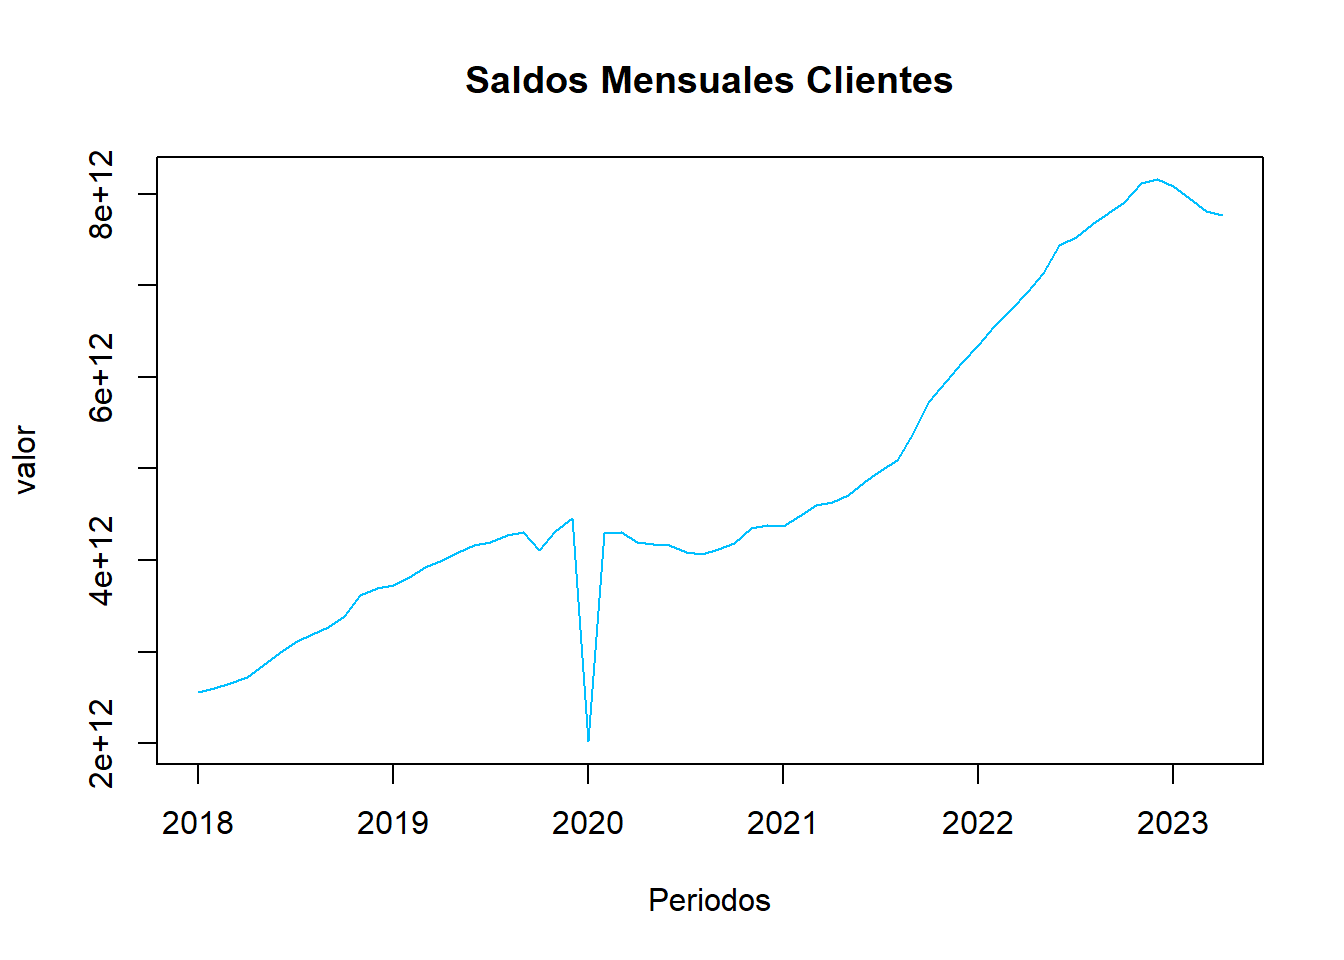
\includegraphics{bookdown-demo_files/figure-latex/unnamed-chunk-3-1.pdf}

\hypertarget{analisis-grafica-de-serie}{%
\subsection{Analisis Grafica de serie}\label{analisis-grafica-de-serie}}

Después de graficar la serie de tiempo, podemos observar ciertas características que nos brindan información valiosa. Por ejemplo, en el primer periodo del 2020, podemos notar un pico descendente en el saldo, lo que podría sugerir un posible error en el registro de los datos históricos.

Por otro lado, al examinar el comportamiento general de la serie de tiempo, se observa un aumento en la utilización de los productos a lo largo de los años, especialmente marcado a partir de la mitad del 2020. Este aumento podría deberse a factores como la pandemia y el desempleo, que podrían haber influido en la demanda de estos productos.

\hypertarget{chequeos-basicos-para-confirmar-la-estructura-del-contenedor-ts}{%
\subsection{Chequeos basicos para confirmar la estructura del contenedor ts}\label{chequeos-basicos-para-confirmar-la-estructura-del-contenedor-ts}}

\begin{verbatim}
## [1] "El tipo de datos del df indice.ts es: "
\end{verbatim}

\begin{verbatim}
## [1] "ts"
\end{verbatim}

\begin{verbatim}
## [1] "La serie de tiempo indice.ts empieza en: "
\end{verbatim}

\begin{verbatim}
## [1] 2018    1
\end{verbatim}

\begin{verbatim}
## [1] "La serie de tiempo indice.ts termina en: "
\end{verbatim}

\begin{verbatim}
## [1] 2023    4
\end{verbatim}

\hypertarget{analisis-descriptivo}{%
\section{Analisis Descriptivo}\label{analisis-descriptivo}}

\hypertarget{grafica-de-rezagos}{%
\subsection{Grafica de Rezagos}\label{grafica-de-rezagos}}

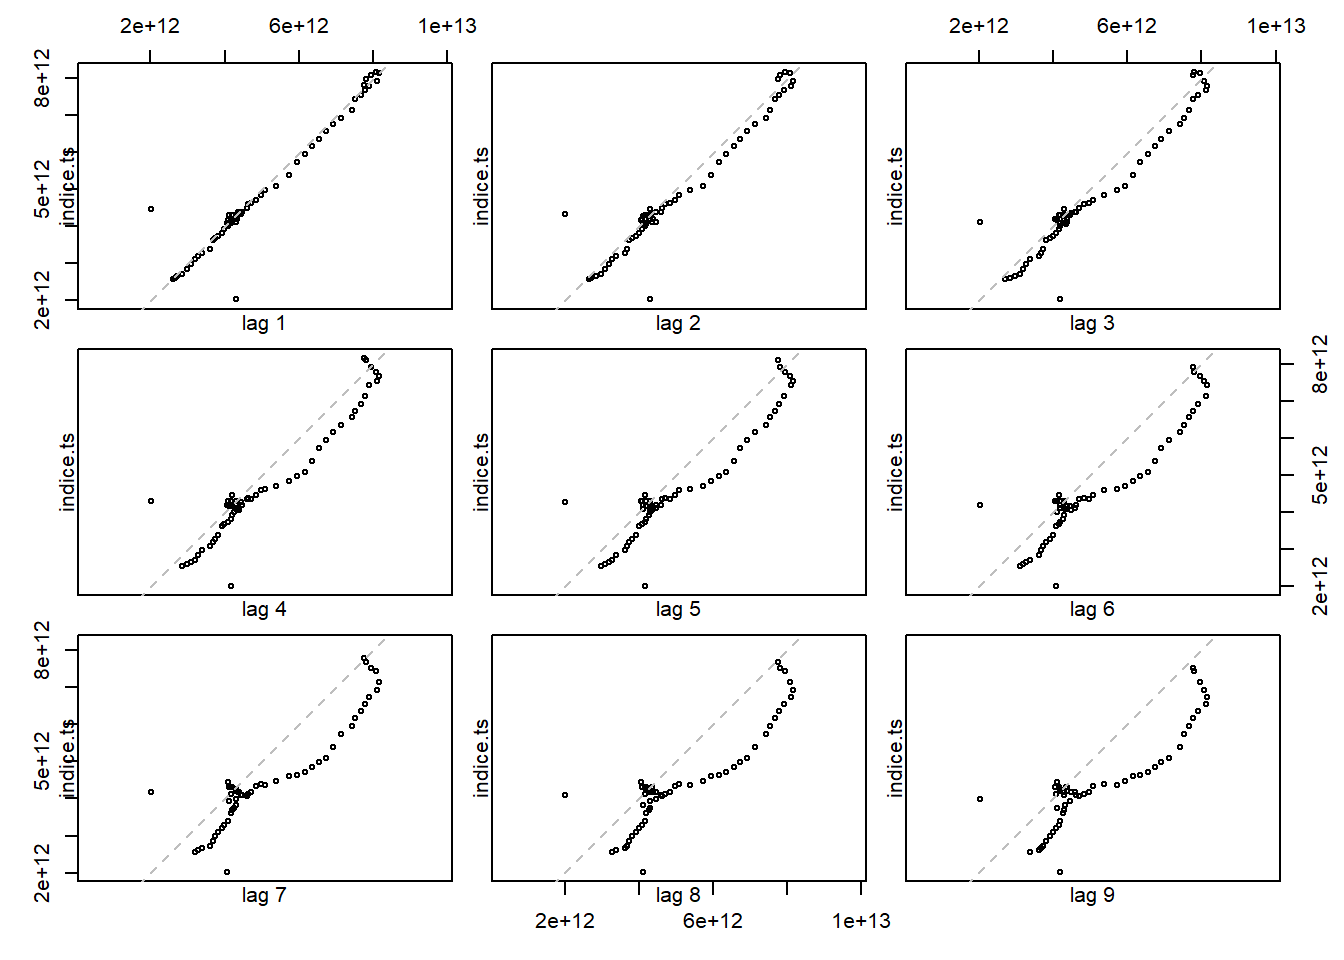
\includegraphics{bookdown-demo_files/figure-latex/unnamed-chunk-5-1.pdf}
Conclusion: Se observa con claridad que existe una tendencia positiva. Esto sugiere una posible transformacion en una etapa posterior del analisis.

\hypertarget{media-movil}{%
\subsection{Media Movil}\label{media-movil}}

Crearemos a continuacion 3 medias moviles para el objeto ts. Estas tendran 3, 5 y 7 periodos para su calculo.

\begin{verbatim}
## Media Movil con 3 meses:  2.60569e+12 2.657587e+12 2.741279e+12 2.852323e+12 2.980516e+12 3.095026e+12 3.19034e+12 3.287521e+12 3.427851e+12 3.567132e+12 3.679831e+12 3.744369e+12 3.822086e+12 3.909977e+12 4.004003e+12 4.084338e+12 4.151794e+12 4.210161e+12 4.257812e+12 4.229589e+12 4.24496e+12 4.294346e+12 3.597313e+12 3.591264e+12 3.540826e+12 4.265159e+12 4.225603e+12 4.179019e+12 4.141387e+12 4.104963e+12 4.090461e+12 4.123917e+12 4.216171e+12 4.303925e+12 4.366066e+12 4.410497e+12 4.480783e+12 4.566974e+12 4.642901e+12 4.72671e+12 4.845379e+12 4.973983e+12 5.153753e+12 5.402739e+12 5.690788e+12 5.950428e+12 6.157316e+12 6.357342e+12 6.549048e+12 6.740214e+12 6.932456e+12 7.164445e+12 7.365887e+12 7.545111e+12 7.662862e+12 7.787577e+12 7.935987e+12 8.057696e+12 8.117688e+12 8.062904e+12 7.949162e+12 7.843058e+12
\end{verbatim}

\begin{verbatim}
## Media Movil con 5 meses:  2.677519e+12 2.762363e+12 2.862556e+12 2.97112e+12 3.082015e+12 3.190301e+12 3.316437e+12 3.433984e+12 3.541184e+12 3.648854e+12 3.754723e+12 3.830459e+12 3.910977e+12 3.997427e+12 4.074914e+12 4.143823e+12 4.206128e+12 4.210266e+12 4.240195e+12 4.29166e+12 3.842557e+12 3.840266e+12 3.878402e+12 3.854676e+12 3.79902e+12 4.227426e+12 4.18475e+12 4.137503e+12 4.122607e+12 4.123739e+12 4.159794e+12 4.22013e+12 4.2804e+12 4.351815e+12 4.434249e+12 4.490882e+12 4.555201e+12 4.650636e+12 4.751812e+12 4.851121e+12 5.002703e+12 5.207714e+12 5.429568e+12 5.665732e+12 5.917714e+12 6.151721e+12 6.353518e+12 6.54737e+12 6.740937e+12 6.957795e+12 7.152497e+12 7.338575e+12 7.511384e+12 7.66557e+12 7.8015e+12 7.92647e+12 8.009116e+12 8.041526e+12 8.023421e+12 7.953359e+12
\end{verbatim}

\begin{verbatim}
## Media Movil con 7 meses:  2.782362e+12 2.872921e+12 2.968758e+12 3.074575e+12 3.203034e+12 3.322694e+12 3.429222e+12 3.5304e+12 3.634291e+12 3.737637e+12 3.837463e+12 3.915643e+12 3.988207e+12 4.064748e+12 4.13569e+12 4.162851e+12 4.208312e+12 4.260123e+12 3.954126e+12 3.968084e+12 3.973265e+12 3.957274e+12 3.966376e+12 3.945005e+12 3.89172e+12 4.183941e+12 4.158946e+12 4.141617e+12 4.162946e+12 4.192513e+12 4.221779e+12 4.278279e+12 4.353579e+12 4.426e+12 4.5007e+12 4.572381e+12 4.658052e+12 4.761236e+12 4.89092e+12 5.053176e+12 5.242871e+12 5.451288e+12 5.666292e+12 5.890855e+12 6.126316e+12 6.346204e+12 6.546447e+12 6.757883e+12 6.952829e+12 7.141217e+12 7.317392e+12 7.483628e+12 7.653691e+12 7.799638e+12 7.89216e+12 7.952412e+12 7.972803e+12 7.969387e+12
\end{verbatim}

Veamos como es el comportamiento de las mismas en comparacion con los datos originales de la serie de tiempo.

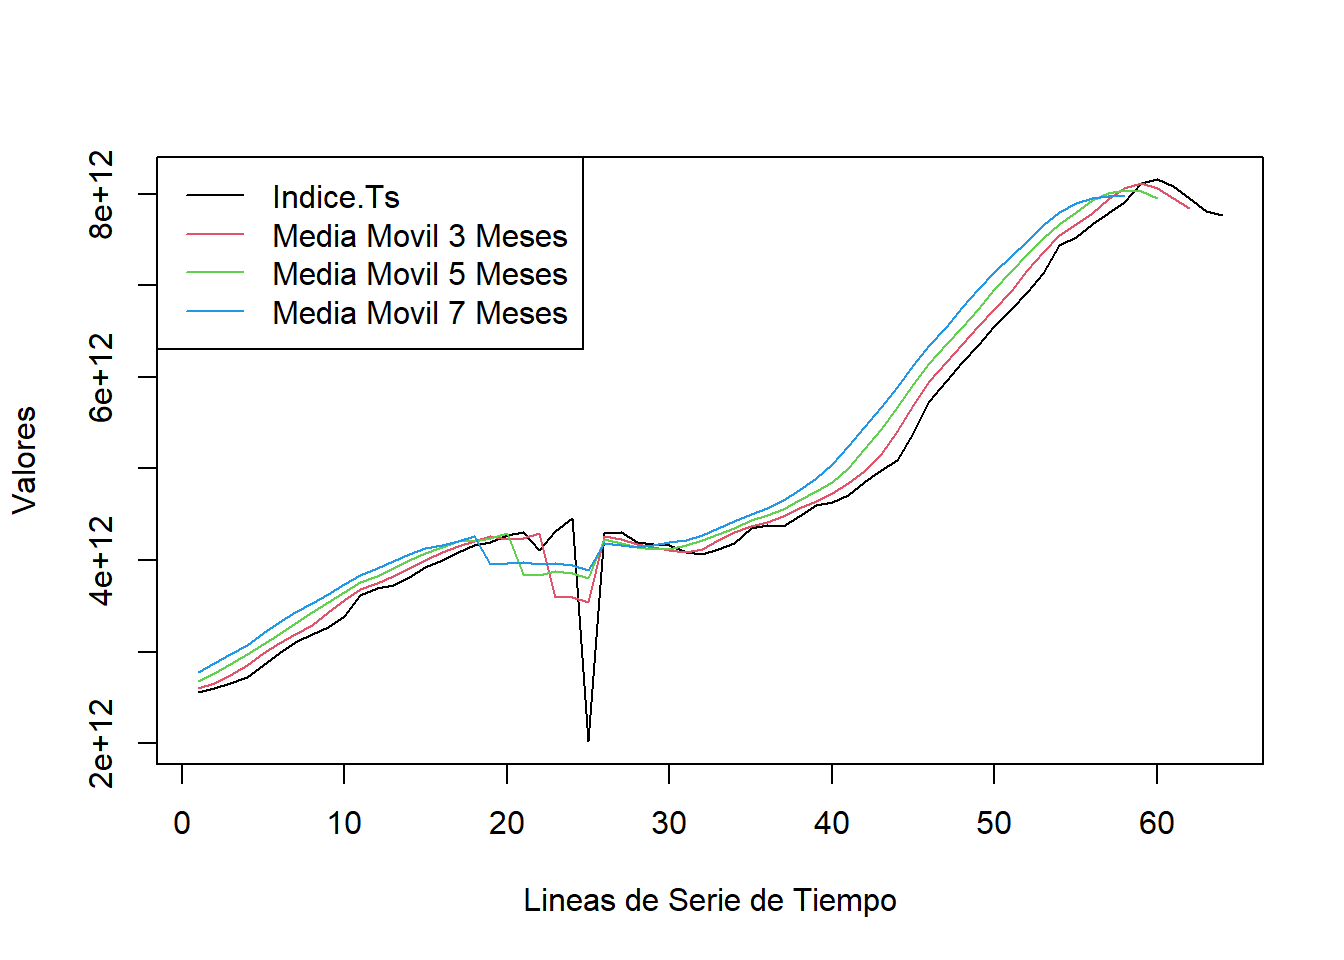
\includegraphics{bookdown-demo_files/figure-latex/unnamed-chunk-7-1.pdf}

\hypertarget{estacionalidad-y-descomposicion}{%
\chapter{Estacionalidad y Descomposicion}\label{estacionalidad-y-descomposicion}}

\hypertarget{Estacion}{%
\section{Estacionalidad}\label{Estacion}}

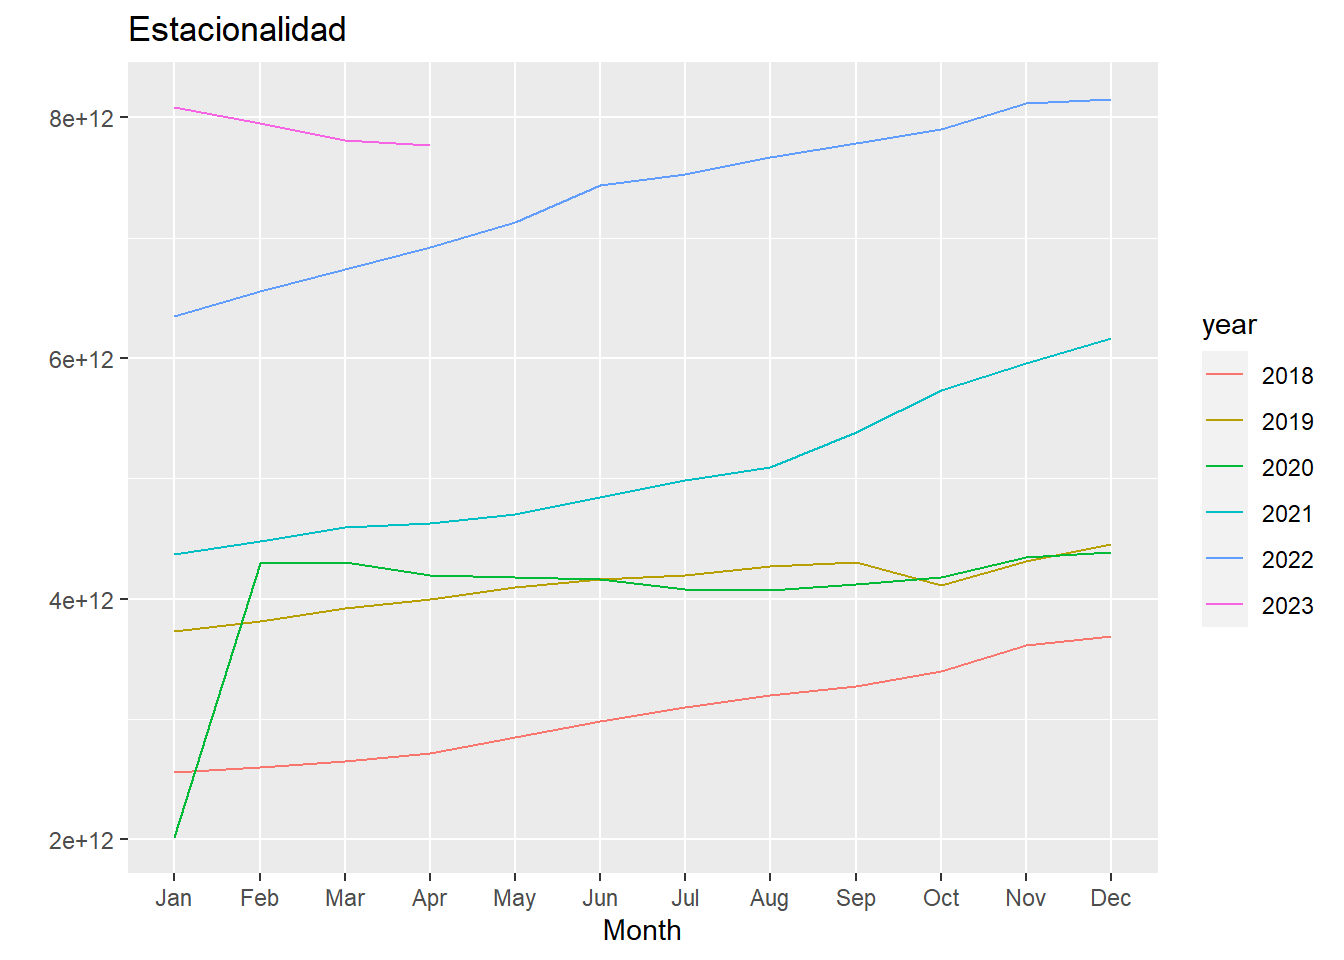
\includegraphics{bookdown-demo_files/figure-latex/unnamed-chunk-8-1.pdf}

\hypertarget{analisis-inicial}{%
\subsection{Analisis Inicial}\label{analisis-inicial}}

Según el análisis de estacionalidad anual, se observa que la utilización de los productos del banco fue moderada en los años 2018 y 2019, tal como se evidencia en las líneas trazadas para esos años. En el 2020, se observa un pico en la utilización que podría indicar un posible error en la recolección de datos. Posteriormente, se observa una pequeña disminución que posiblemente se debió al inicio de la pandemia y la incertidumbre mundial. A partir de septiembre de 2020, se observa un incremento continuo en la utilización para los años 2021 y 2022, posiblemente como resultado de la duración de la pandemia y la crisis económica global.

En el año 2023, se comienza a evidenciar una disminución en la utilización de los productos del banco, lo que podría deberse al alza de las tasas de interés o a un cambio en el comportamiento de los clientes. Es importante mencionar que se requiere un análisis más detallado para determinar las causas precisas de esta disminución.

\hypertarget{descomposicion-del-objeto-y-analisis}{%
\section{Descomposicion del objeto y analisis}\label{descomposicion-del-objeto-y-analisis}}

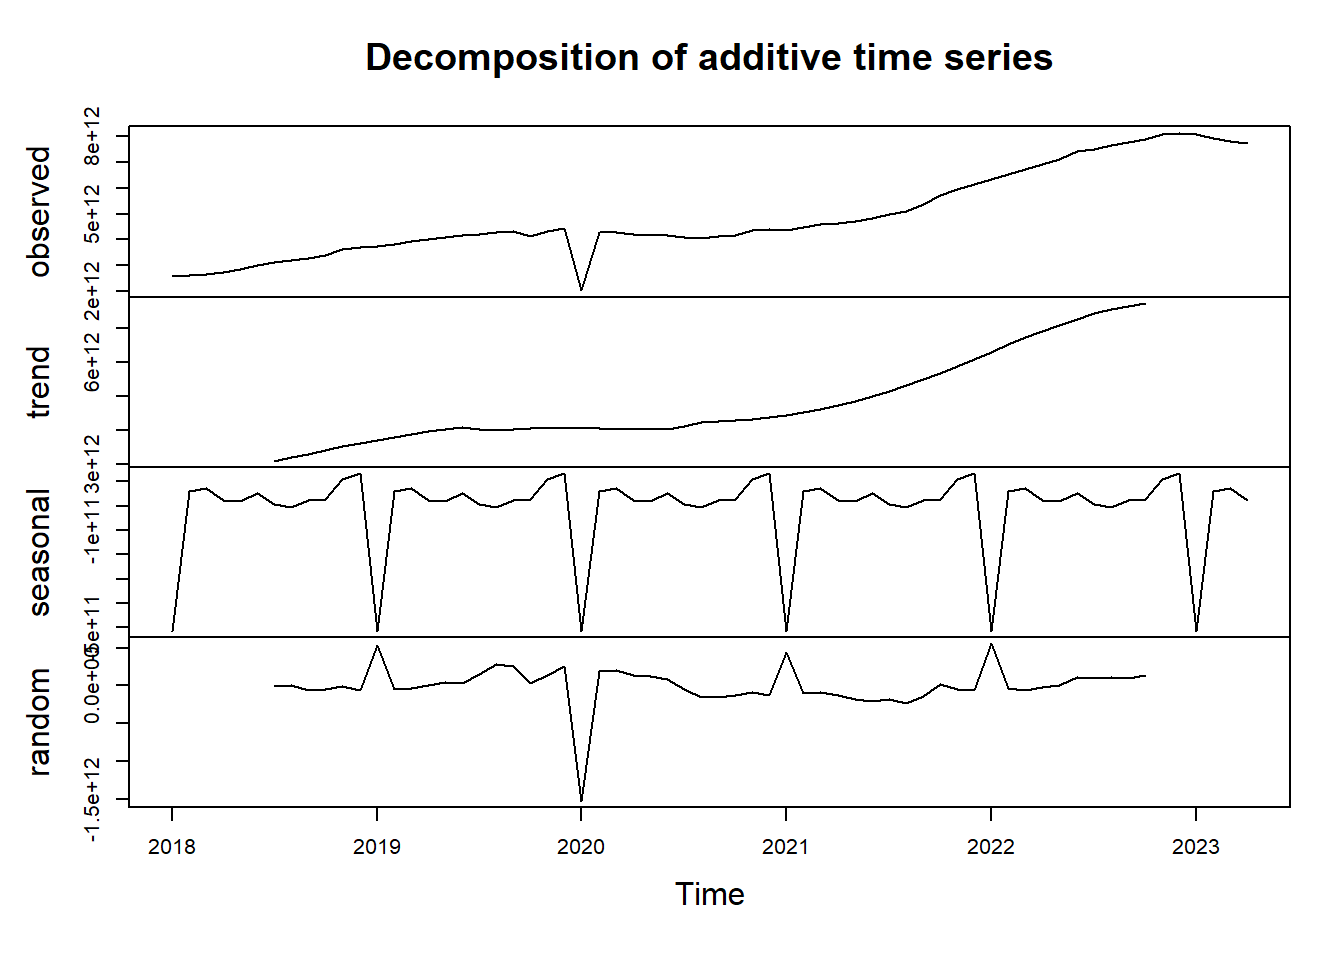
\includegraphics{bookdown-demo_files/figure-latex/unnamed-chunk-9-1.pdf}

A pesar de presentar un patron recurrente en el componente de estacionalidad, se puede observar un trend en la serie de datos. De igual manera el error no se ve aleatorio sino que por el contrario, presenta un patron constante. Dicho esto, vamos a comprobar por medio del Augmented Dickery-Fuller test (adf) la estacionalidad del conjunto de datos.

\hypertarget{prueba-de-estacionalidad}{%
\subsection{Prueba de Estacionalidad}\label{prueba-de-estacionalidad}}

\begin{verbatim}
## 
##  Augmented Dickey-Fuller Test
## 
## data:  indice.ts
## Dickey-Fuller = -1.2017, Lag order = 3, p-value = 0.8984
## alternative hypothesis: stationary
\end{verbatim}

De acuerdo al resultado (p-value \textgreater0.05), debemos aceptar la H0 la cual nos confirma la no-estacionalidad del conjunto. Esto quiere decir que el objeto indice.ts requerira una transformacion para su posterior procesamiento en el modelo.

\hypertarget{autocorrelacion}{%
\subsection{Autocorrelacion}\label{autocorrelacion}}

Ahora veamos si existe autocorrelacion total o parcial.(acf y pacf tests)

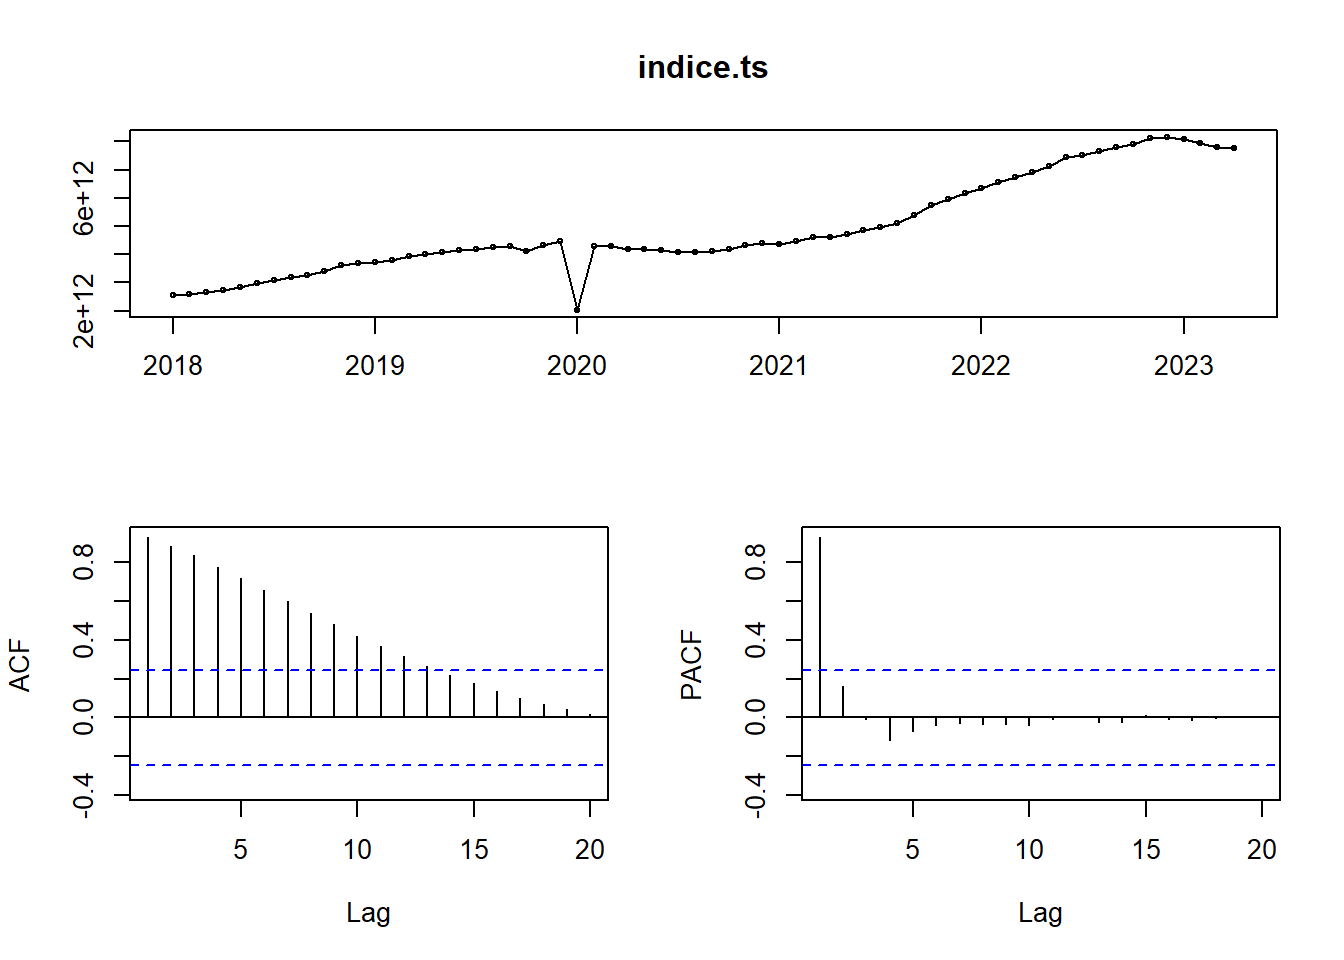
\includegraphics{bookdown-demo_files/figure-latex/unnamed-chunk-11-1.pdf}

Como se puede observar, existe autocorrelacion entre la variable observada lo cual confirma la tendencia en la serie temporal. Por otro lado no evidenciamos autocorrelacion parcial ya que no encontramos picos por fuera del umbral (0.95)

\hypertarget{transformacion}{%
\section{Transformacion}\label{transformacion}}

\begin{verbatim}
## [1] "Ajustamos la estacionalidad de la serie de tiempo por medio del comando seasadj"
\end{verbatim}

\begin{verbatim}
## [1] "Luego removemos la tendencia (trend) con el comando diff"
\end{verbatim}

\begin{verbatim}
## [1] "Grafiquemos la nueva serie de tiempo"
\end{verbatim}

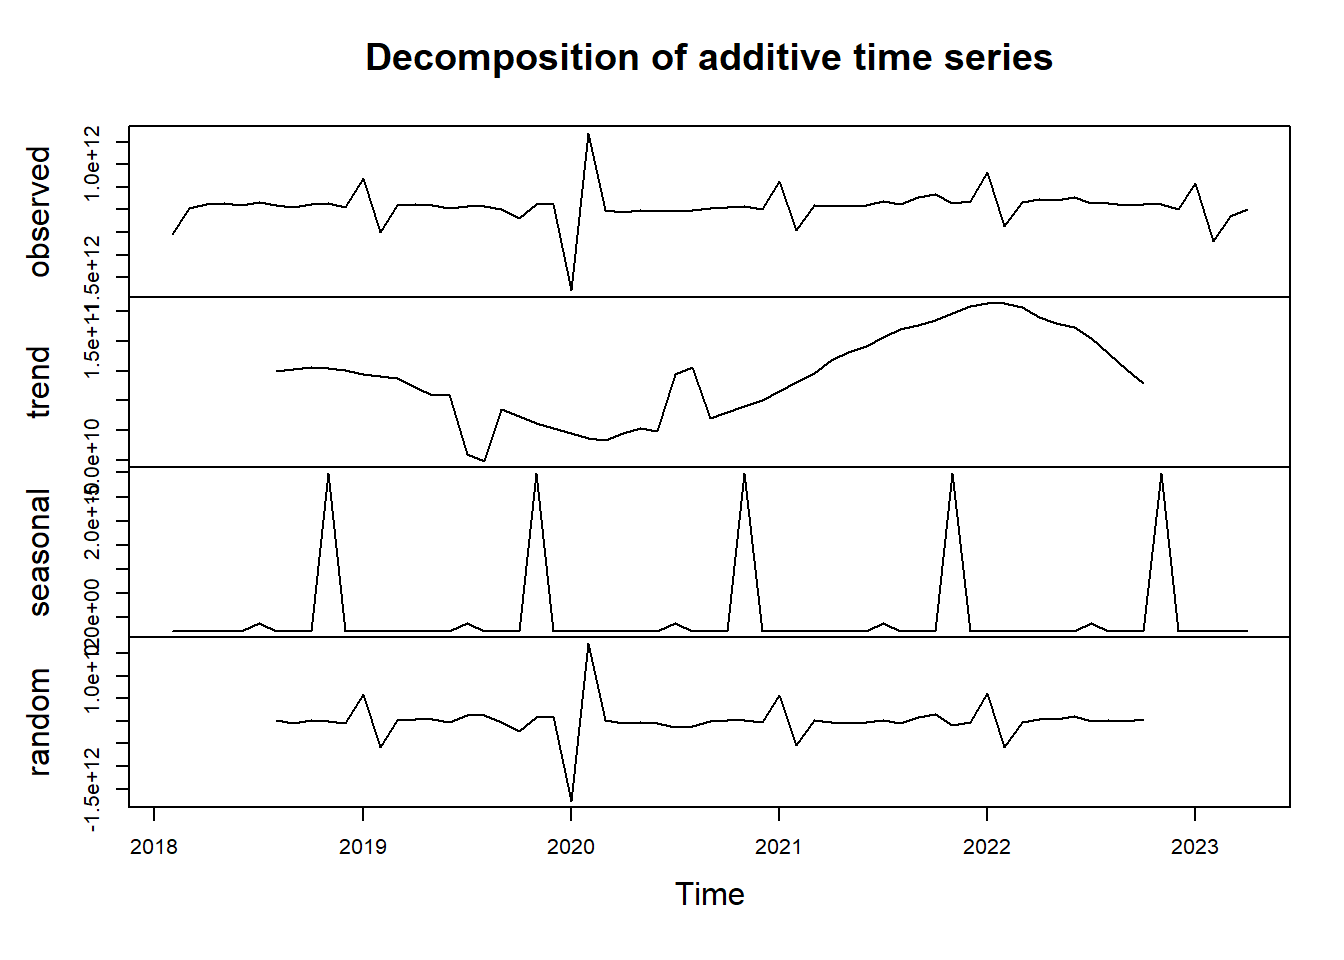
\includegraphics{bookdown-demo_files/figure-latex/unnamed-chunk-12-1.pdf}

\hypertarget{validacion-de-nuestra-nueva-serie-de-tiempo-transformada}{%
\subsection{Validacion de nuestra nueva serie de tiempo transformada}\label{validacion-de-nuestra-nueva-serie-de-tiempo-transformada}}

\begin{verbatim}
## 
##  Augmented Dickey-Fuller Test
## 
## data:  modelo_ts
## Dickey-Fuller = -3.7052, Lag order = 3, p-value = 0.0316
## alternative hypothesis: stationary
\end{verbatim}

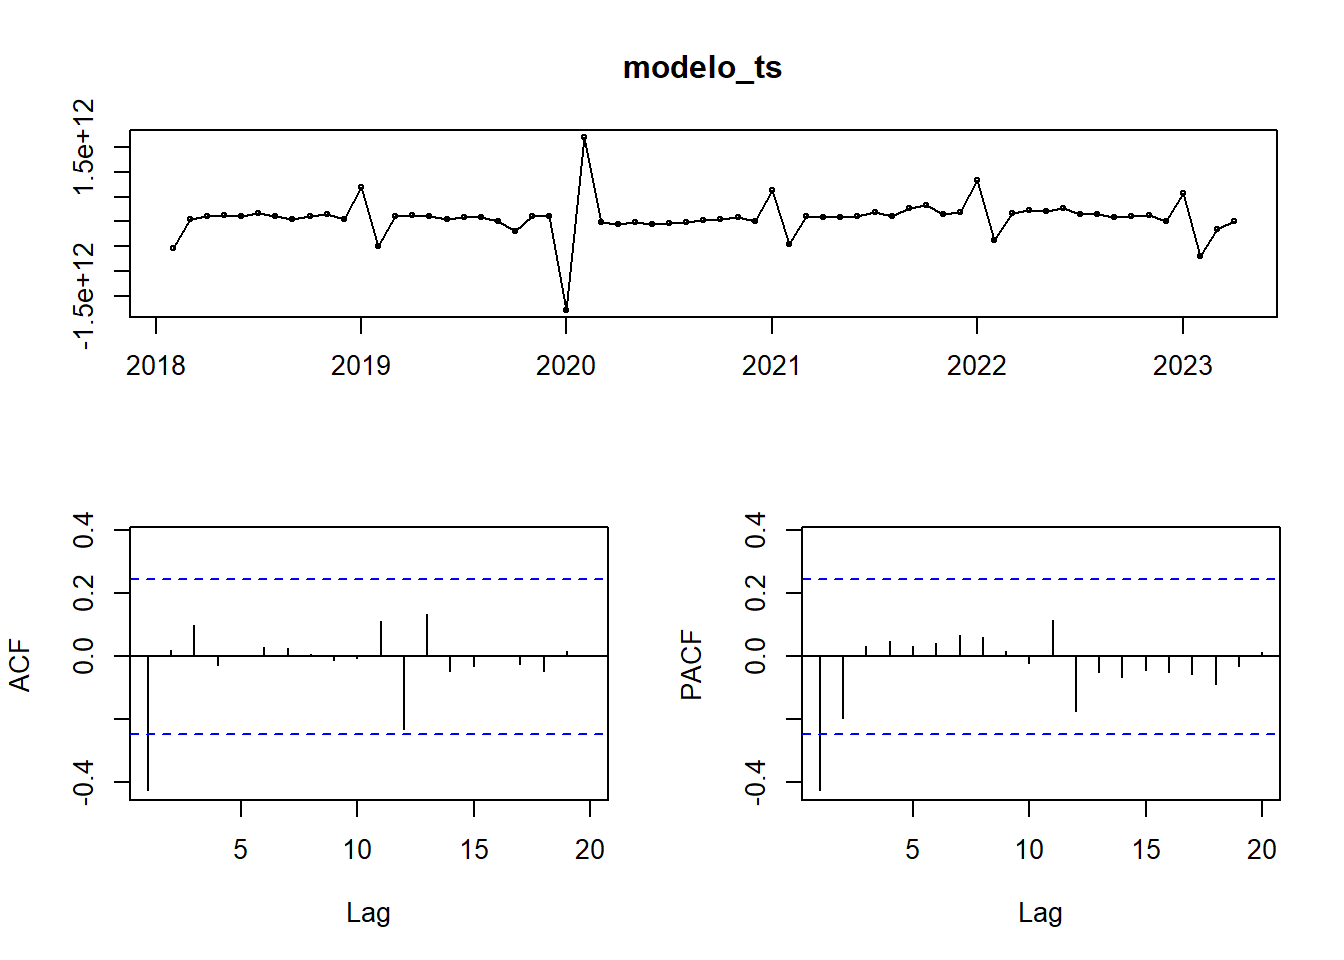
\includegraphics{bookdown-demo_files/figure-latex/unnamed-chunk-13-1.pdf}

se observa que la serie es de tipo estacionaria (p-value=0.0316 \textless{} 0.05), la varianza y la media son de tipo constante, los datos se mueven alrededor de cero (0).

\hypertarget{conclusiones}{%
\section{Conclusiones}\label{conclusiones}}

En conclusión, el análisis de serie de tiempo de la utilización de los productos del banco nos ha permitido identificar patrones y tendencias en su utilización.

A partir del análisis de estacionalidad, se observó que la utilización de los productos del banco ha sido moderada en los años 2018 y 2019, y ha aumentado significativamente en el 2020 y 2021. Además, se evidenció una disminución en la utilización para el año 2023.

La descomposición de la serie de tiempo nos permitió identificar las componentes de tendencia, estacionalidad y error, y su análisis nos ha brindado una mejor comprensión de los patrones y comportamientos observados en la utilización de los productos del banco.

Asimismo, se realizó la diferenciación de la serie de tiempo para eliminar la tendencia y hacer la serie estacionaria. Esto nos permitió obtener una serie de tiempo más homogénea, y por lo tanto, una mejor visualización de las fluctuaciones en la utilización de los productos del banco.Como resultado, la nueva serie de tiempo sera nuestra base para la implementacion de modelos de pronostico de los productos observados.

\hypertarget{holt-wintershw-y-suavizamiento-exp.}{%
\chapter{Holt-Winters(HW) y Suavizamiento Exp.}\label{holt-wintershw-y-suavizamiento-exp.}}

\hypertarget{hw}{%
\section{HW}\label{hw}}

Para aplicar la metodología de Holt-Winters y suavizamiento exponencial a la serie de tiempo indice.ts, podemos utilizar las funciones correspondientes de R. La metodología de Holt-Winters es adecuada para modelar series de tiempo con componentes de tendencia y estacionalidad.
El resultado del modelo Holt-Winters proporciona las componentes de tendencia (trend), estacionalidad (seasonal) y residuos (residuals). Estas componentes ayudan a comprender los patrones y la estructura de la serie de tiempo.

A continuación, se muestra cómo aplicar ambas técnicas a la serie de tiempo indice.ts:

\begin{Shaded}
\begin{Highlighting}[]
\CommentTok{\# Aplicar la metodología de Holt{-}Winters}
\NormalTok{hw\_model }\OtherTok{\textless{}{-}} \FunctionTok{HoltWinters}\NormalTok{(indice.ts)}

\CommentTok{\# Obtener las componentes del modelo (tendencia, estacionalidad y residuos)}
\NormalTok{trend }\OtherTok{\textless{}{-}}\NormalTok{ hw\_model}\SpecialCharTok{$}\NormalTok{components}\SpecialCharTok{$}\NormalTok{trend}
\NormalTok{seasonal }\OtherTok{\textless{}{-}}\NormalTok{ hw\_model}\SpecialCharTok{$}\NormalTok{components}\SpecialCharTok{$}\NormalTok{seasonal}
\NormalTok{residuals }\OtherTok{\textless{}{-}}\NormalTok{ hw\_model}\SpecialCharTok{$}\NormalTok{components}\SpecialCharTok{$}\NormalTok{random}

\CommentTok{\# Imprimir las componentes}
\FunctionTok{print}\NormalTok{(}\StringTok{"Tendencia:"}\NormalTok{)}
\end{Highlighting}
\end{Shaded}

\begin{verbatim}
## [1] "Tendencia:"
\end{verbatim}

\begin{Shaded}
\begin{Highlighting}[]
\FunctionTok{print}\NormalTok{(trend)}
\end{Highlighting}
\end{Shaded}

\begin{verbatim}
## NULL
\end{verbatim}

\begin{Shaded}
\begin{Highlighting}[]
\FunctionTok{print}\NormalTok{(}\StringTok{"Estacionalidad:"}\NormalTok{)}
\end{Highlighting}
\end{Shaded}

\begin{verbatim}
## [1] "Estacionalidad:"
\end{verbatim}

\begin{Shaded}
\begin{Highlighting}[]
\FunctionTok{print}\NormalTok{(seasonal)}
\end{Highlighting}
\end{Shaded}

\begin{verbatim}
## NULL
\end{verbatim}

\begin{Shaded}
\begin{Highlighting}[]
\FunctionTok{print}\NormalTok{(}\StringTok{"Residuos:"}\NormalTok{)}
\end{Highlighting}
\end{Shaded}

\begin{verbatim}
## [1] "Residuos:"
\end{verbatim}

\begin{Shaded}
\begin{Highlighting}[]
\FunctionTok{print}\NormalTok{(residuals)}
\end{Highlighting}
\end{Shaded}

\begin{verbatim}
## NULL
\end{verbatim}

Suavizamiento exponencial:
El suavizamiento exponencial,es útil para suavizar las fluctuaciones en la serie de tiempo.

\begin{Shaded}
\begin{Highlighting}[]
\CommentTok{\# Aplicar suavizamiento exponencial}
\NormalTok{smoothed }\OtherTok{\textless{}{-}} \FunctionTok{HoltWinters}\NormalTok{(indice.ts, }\AttributeTok{beta =} \ConstantTok{FALSE}\NormalTok{, }\AttributeTok{gamma =} \ConstantTok{FALSE}\NormalTok{)}\SpecialCharTok{$}\NormalTok{fitted}

\CommentTok{\# Imprimir la serie de tiempo suavizada}
\FunctionTok{print}\NormalTok{(}\StringTok{"Serie de tiempo suavizada:"}\NormalTok{)}
\end{Highlighting}
\end{Shaded}

\begin{verbatim}
## [1] "Serie de tiempo suavizada:"
\end{verbatim}

\begin{Shaded}
\begin{Highlighting}[]
\FunctionTok{print}\NormalTok{(smoothed)}
\end{Highlighting}
\end{Shaded}

\begin{verbatim}
##                  xhat        level
## Feb 2018 2.562223e+12 2.562223e+12
## Mar 2018 2.586847e+12 2.586847e+12
## Apr 2018 2.628483e+12 2.628483e+12
## May 2018 2.684505e+12 2.684505e+12
## Jun 2018 2.789807e+12 2.789807e+12
## Jul 2018 2.912985e+12 2.912985e+12
## Aug 2018 3.031696e+12 3.031696e+12
## Sep 2018 3.134705e+12 3.134705e+12
## Oct 2018 3.220952e+12 3.220952e+12
## Nov 2018 3.329376e+12 3.329376e+12
## Dec 2018 3.509629e+12 3.509629e+12
## Jan 2019 3.622760e+12 3.622760e+12
## Feb 2019 3.691275e+12 3.691275e+12
## Mar 2019 3.766110e+12 3.766110e+12
## Apr 2019 3.864626e+12 3.864626e+12
## May 2019 3.946802e+12 3.946802e+12
## Jun 2019 4.038270e+12 4.038270e+12
## Jul 2019 4.117271e+12 4.117271e+12
## Aug 2019 4.167952e+12 4.167952e+12
## Sep 2019 4.230574e+12 4.230574e+12
## Oct 2019 4.278661e+12 4.278661e+12
## Nov 2019 4.175205e+12 4.175205e+12
## Dec 2019 4.262169e+12 4.262169e+12
## Jan 2020 4.383274e+12 4.383274e+12
## Feb 2020 2.904388e+12 2.904388e+12
## Mar 2020 3.776045e+12 3.776045e+12
## Apr 2020 4.106880e+12 4.106880e+12
## May 2020 4.162333e+12 4.162333e+12
## Jun 2020 4.171658e+12 4.171658e+12
## Jul 2020 4.167133e+12 4.167133e+12
## Aug 2020 4.114122e+12 4.114122e+12
## Sep 2020 4.085198e+12 4.085198e+12
## Oct 2020 4.107579e+12 4.107579e+12
## Nov 2020 4.154747e+12 4.154747e+12
## Dec 2020 4.273742e+12 4.273742e+12
## Jan 2021 4.342927e+12 4.342927e+12
## Feb 2021 4.359448e+12 4.359448e+12
## Mar 2021 4.433712e+12 4.433712e+12
## Apr 2021 4.534775e+12 4.534775e+12
## May 2021 4.593094e+12 4.593094e+12
## Jun 2021 4.663684e+12 4.663684e+12
## Jul 2021 4.778186e+12 4.778186e+12
## Aug 2021 4.907038e+12 4.907038e+12
## Sep 2021 5.022646e+12 5.022646e+12
## Oct 2021 5.250122e+12 5.250122e+12
## Nov 2021 5.551251e+12 5.551251e+12
## Dec 2021 5.804630e+12 5.804630e+12
## Jan 2022 6.030187e+12 6.030187e+12
## Feb 2022 6.231463e+12 6.231463e+12
## Mar 2022 6.434645e+12 6.434645e+12
## Apr 2022 6.625813e+12 6.625813e+12
## May 2022 6.813229e+12 6.813229e+12
## Jun 2022 7.013252e+12 7.013252e+12
## Jul 2022 7.277938e+12 7.277938e+12
## Aug 2022 7.435413e+12 7.435413e+12
## Sep 2022 7.582495e+12 7.582495e+12
## Oct 2022 7.711882e+12 7.711882e+12
## Nov 2022 7.831897e+12 7.831897e+12
## Dec 2022 8.009515e+12 8.009515e+12
## Jan 2023 8.100132e+12 8.100132e+12
## Feb 2023 8.089679e+12 8.089679e+12
## Mar 2023 8.002867e+12 8.002867e+12
## Apr 2023 7.883898e+12 7.883898e+12
\end{verbatim}

La función HoltWinters con los argumentos beta = FALSE y gamma = FALSE aplica el suavizamiento exponencial simple sin considerar la componente de estacionalidad en el modelo.

Al aplicar esta metodología y el suavizamiento exponencial a la serie de tiempo indice.ts, se obtendrá la tendencia, la estacionalidad, los residuos y la serie de tiempo suavizada. Estos resultados ayudarán a comprender la estructura y los patrones de la serie de tiempo.

\begin{Shaded}
\begin{Highlighting}[]
\NormalTok{hw\_model}\OtherTok{=}\FunctionTok{HoltWinters}\NormalTok{(indice.ts, }\AttributeTok{seasonal =} \StringTok{"additive"}\NormalTok{)}
\FunctionTok{plot}\NormalTok{(hw\_model)}
\end{Highlighting}
\end{Shaded}

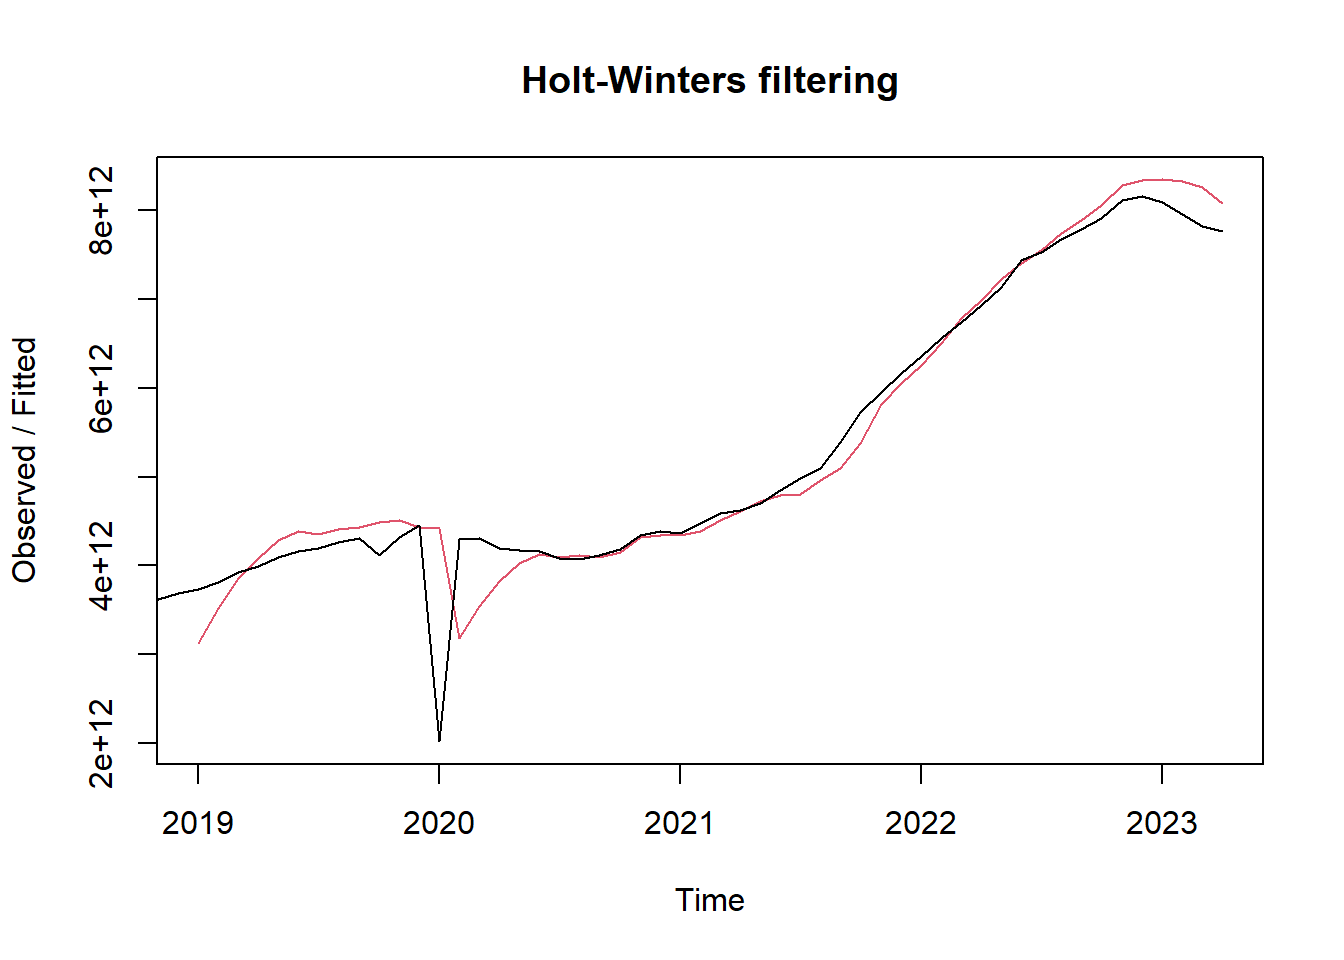
\includegraphics{bookdown-demo_files/figure-latex/unnamed-chunk-16-1.pdf}
Utilizando el comando HoltWinters en R, podemos generar una gráfica en color rojo que representa una serie de datos aproximada a los datos originales en color negro. Cabe destacar que toda serie de tiempo consta de un componente constante, tendencia y estacionalidad. Para ajustar la serie según estas características, realizamos lo siguiente:

\begin{Shaded}
\begin{Highlighting}[]
\FunctionTok{plot}\NormalTok{(}\FunctionTok{fitted}\NormalTok{(hw\_model))}
\end{Highlighting}
\end{Shaded}

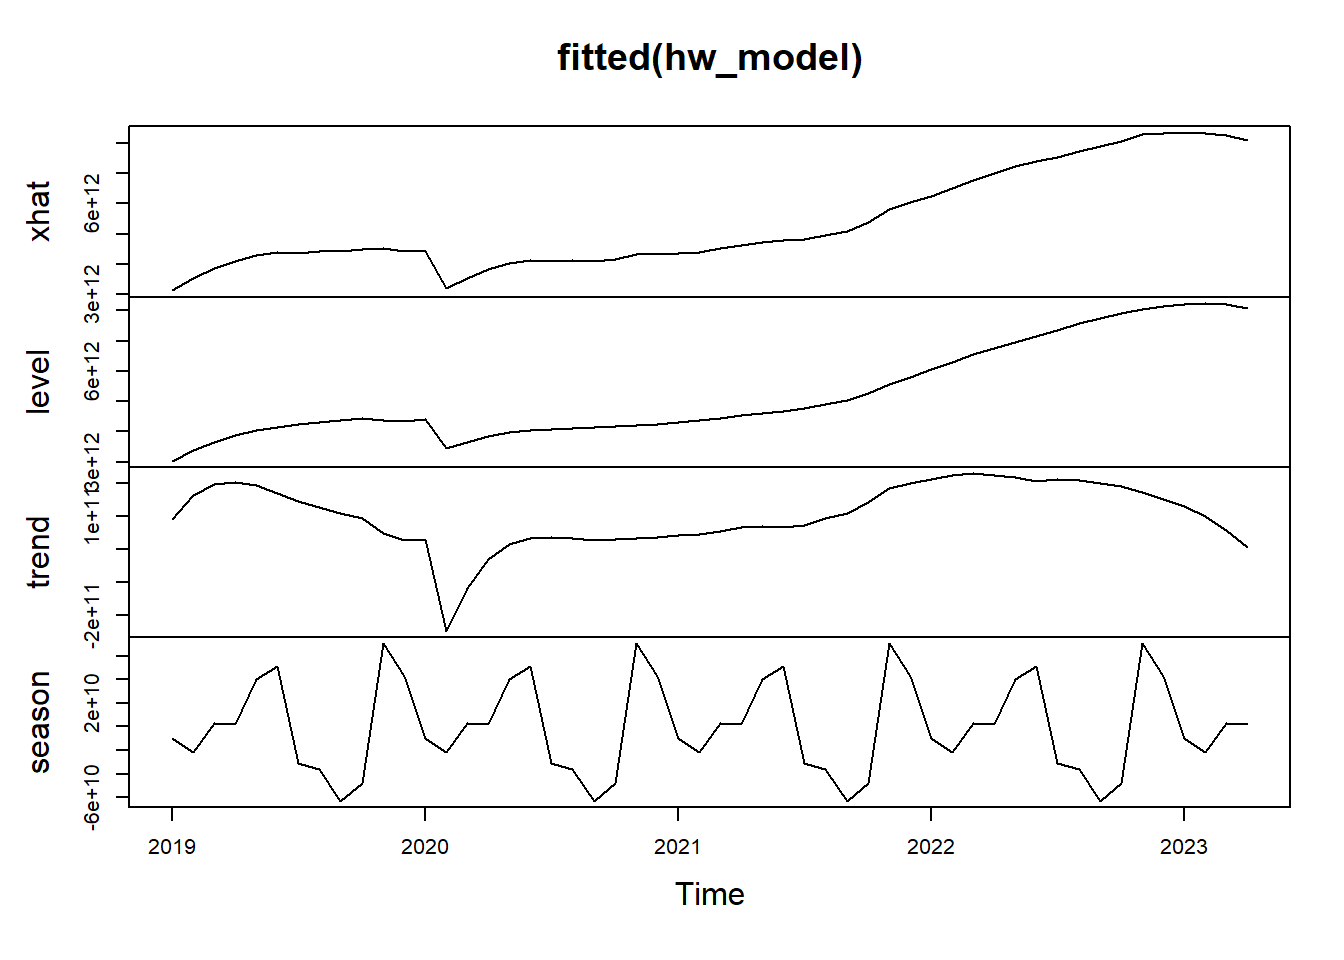
\includegraphics{bookdown-demo_files/figure-latex/unnamed-chunk-17-1.pdf}
En la gráfica se puede observar la descomposición en las cuatro componentes mencionadas previamente.

El método Holt Winters nos permite realizar predicciones utilizando la serie de tiempo. A continuación, se muestra el proceso de generación de predicciones.

\begin{Shaded}
\begin{Highlighting}[]
\NormalTok{pred}\OtherTok{=}\FunctionTok{predict}\NormalTok{(hw\_model, }\DecValTok{12}\NormalTok{, }\AttributeTok{prediction.interval =} \ConstantTok{TRUE}\NormalTok{)}
\NormalTok{pred}
\end{Highlighting}
\end{Shaded}

\begin{verbatim}
##                   fit          upr          lwr
## May 2023 7.958686e+12 8.802116e+12 7.115255e+12
## Jun 2023 7.938280e+12 8.890571e+12 6.985989e+12
## Jul 2023 7.825482e+12 8.920472e+12 6.730492e+12
## Aug 2023 7.788949e+12 9.056689e+12 6.521209e+12
## Sep 2023 7.730847e+12 9.197373e+12 6.264322e+12
## Oct 2023 7.715284e+12 9.403168e+12 6.027400e+12
## Nov 2023 7.802406e+12 9.731469e+12 5.873343e+12
## Dec 2023 7.743702e+12 9.931634e+12 5.555770e+12
## Jan 2024 7.659827e+12 1.012267e+13 5.196985e+12
## Feb 2024 7.617072e+12 1.036958e+13 4.864568e+12
## Mar 2024 7.610883e+12 1.066677e+13 4.554994e+12
## Apr 2024 7.579164e+12 1.095133e+13 4.207002e+12
\end{verbatim}

Se generan predicciones para los próximos 12 meses (May 2023 - Apr 2024) y se procede a graficar la predicción.

\begin{Shaded}
\begin{Highlighting}[]
\FunctionTok{plot}\NormalTok{(hw\_model, pred)}
\end{Highlighting}
\end{Shaded}

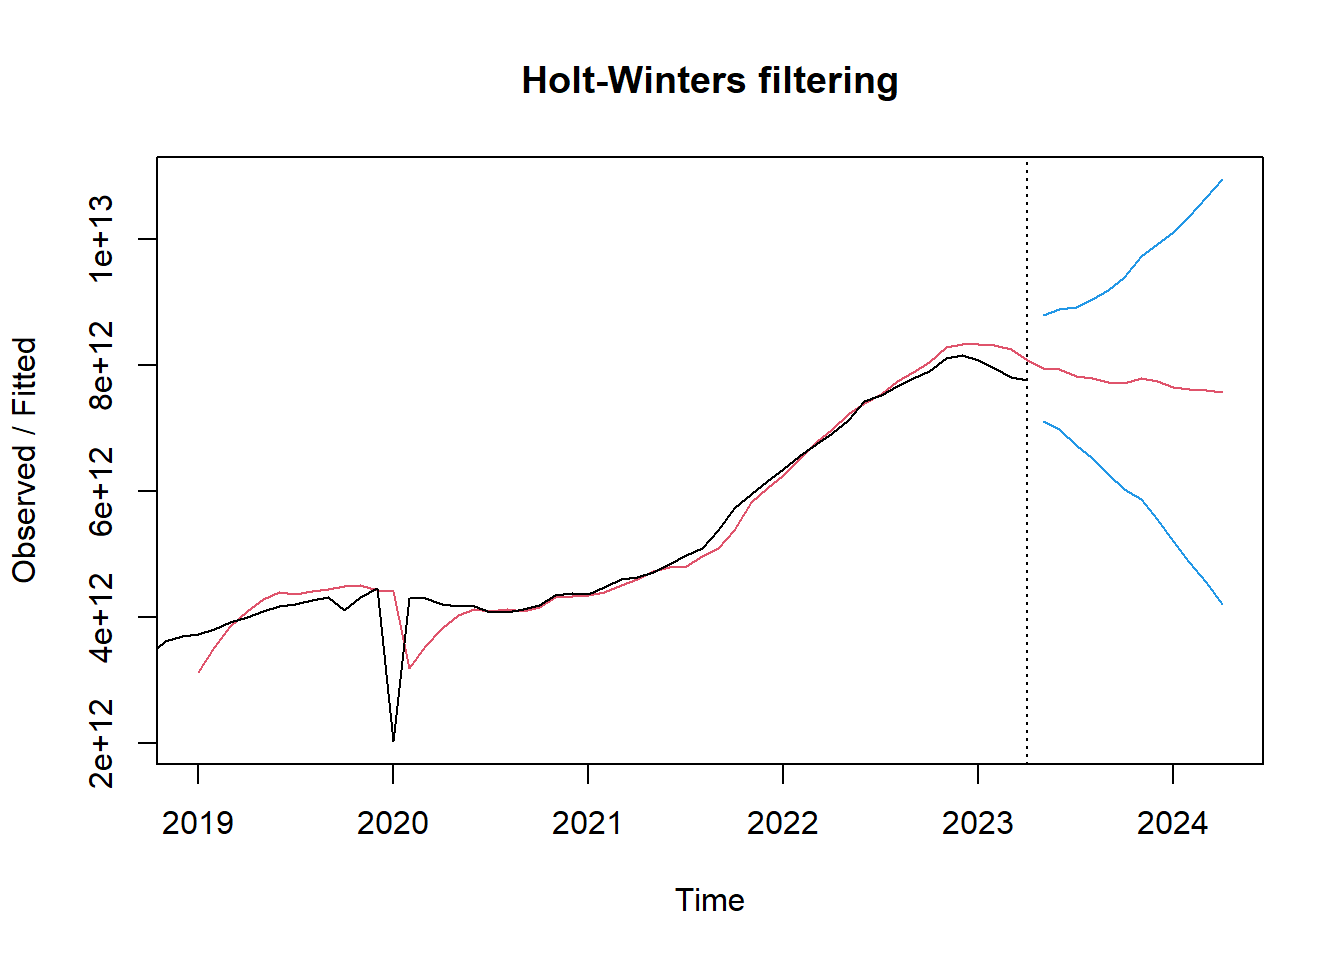
\includegraphics{bookdown-demo_files/figure-latex/unnamed-chunk-19-1.pdf}
En la gráfica se muestran la tendencia de los valores pronosticados junto con sus intervalos de confianza.

Tambien podemos utilizar la funcion hw

\begin{Shaded}
\begin{Highlighting}[]
\CommentTok{\# Calcular el modelo de Holt{-}Winters utilizando la función hw():}
  
\NormalTok{hw\_model1 }\OtherTok{\textless{}{-}} \FunctionTok{HoltWinters}\NormalTok{(indice.ts)}
\NormalTok{hw\_model1}
\end{Highlighting}
\end{Shaded}

\begin{verbatim}
## Holt-Winters exponential smoothing with trend and additive seasonal component.
## 
## Call:
## HoltWinters(x = indice.ts)
## 
## Smoothing parameters:
##  alpha: 0.407578
##  beta : 0.2861578
##  gamma: 0
## 
## Coefficients:
##              [,1]
## a   7949360142242
## b    -31047949847
## s1    40373454460
## s2    51015741884
## s3   -30734639955
## s4   -36219767637
## s5   -63272955789
## s6   -47788675079
## s7    70381305327
## s8    42725269292
## s9   -10101155804
## s10  -21808809060
## s11    3050492943
## s12    2379739417
\end{verbatim}

se generan predicciones para los próximos 12 periodos.

\begin{Shaded}
\begin{Highlighting}[]
\CommentTok{\# Obtener las predicciones del modelo para un horizonte de tiempo determinado:}
\FunctionTok{library}\NormalTok{(forecast) }
\NormalTok{predictions }\OtherTok{\textless{}{-}} \FunctionTok{forecast}\NormalTok{(hw\_model1, }\AttributeTok{h =} \DecValTok{12}\NormalTok{)  }\CommentTok{\# Predicciones para los próximos 12 periodos}
\end{Highlighting}
\end{Shaded}

Esto generará un gráfico que muestra la serie de tiempo original y las predicciones del modelo de Holt-Winters.

\begin{Shaded}
\begin{Highlighting}[]
\FunctionTok{plot}\NormalTok{(hw\_model1, }\AttributeTok{main =} \StringTok{"Modelo de Holt{-}Winters: Serie de tiempo y predicciones"}\NormalTok{)}
\FunctionTok{lines}\NormalTok{(predictions}\SpecialCharTok{$}\NormalTok{mean, }\AttributeTok{col =} \StringTok{"blue"}\NormalTok{)}
\FunctionTok{legend}\NormalTok{(}\StringTok{"bottomright"}\NormalTok{, }\AttributeTok{legend =} \FunctionTok{c}\NormalTok{(}\StringTok{"Serie de tiempo"}\NormalTok{, }\StringTok{"Predicciones"}\NormalTok{), }\AttributeTok{col =} \FunctionTok{c}\NormalTok{(}\StringTok{"black"}\NormalTok{, }\StringTok{"blue"}\NormalTok{), }\AttributeTok{lty =} \DecValTok{1}\NormalTok{)}
\end{Highlighting}
\end{Shaded}

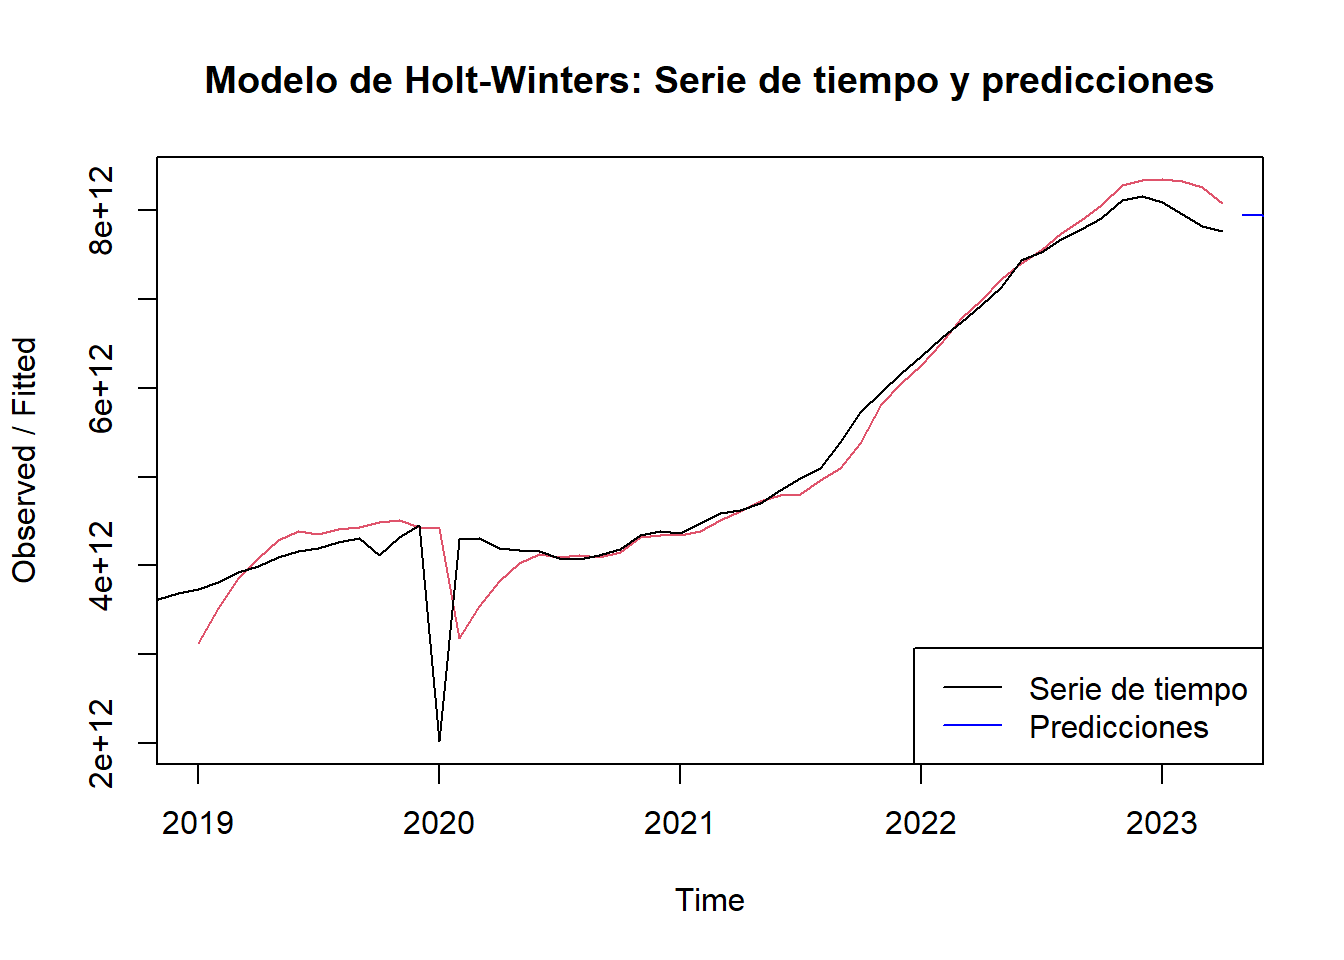
\includegraphics{bookdown-demo_files/figure-latex/unnamed-chunk-22-1.pdf}

\hypertarget{modelo-arima}{%
\chapter{Modelo ARIMA}\label{modelo-arima}}

\#\#Metodología Box-Jenkins para identificar modelos autoregresivos integrados de media móvil (ARIMA) para analizar y predecir valores futuros de serie de tiempo.

En esta seccion, intentaremos abordar el algoritmo ARIMA dentro de la serie de tiempo. Primero consrtruiremos el modelo optimo AR, luego MA y posteriormente utilizaremos la funcion Autoarima para encontrar los parametros optimos.

\hypertarget{modelos}{%
\section{Modelos}\label{modelos}}

\begin{verbatim}
## -- Attaching packages ---------------------------------------------- fpp2 2.5 --
\end{verbatim}

\begin{verbatim}
## v fma       2.5     v expsmooth 2.3
\end{verbatim}

\begin{verbatim}
## 
\end{verbatim}

\begin{verbatim}
## [1] "Verificamos la estacionalidad del modelo (p<0.05)"
\end{verbatim}

\begin{verbatim}
## 
##  Augmented Dickey-Fuller Test
## 
## data:  modelo_ts
## Dickey-Fuller = -3.7052, Lag order = 3, p-value = 0.0316
## alternative hypothesis: stationary
\end{verbatim}

Como se puede observar, se rechaza la hipotesis ho y aceptamos la alterna. xxxxxxx , dentro de nuestros modelos ARIMA podemos asegurar que el parametro d = 0.

\hypertarget{modelo-basado-solamente-en-auro-regresion-ar.-debemos-ubicar-los-parametros-d-y-q-en-0.}{%
\subsection{Modelo basado solamente en Auro Regresion (AR). Debemos ubicar los parametros d y q en 0.}\label{modelo-basado-solamente-en-auro-regresion-ar.-debemos-ubicar-los-parametros-d-y-q-en-0.}}

Por medio del analisis ACF y PACF verificamos los lags

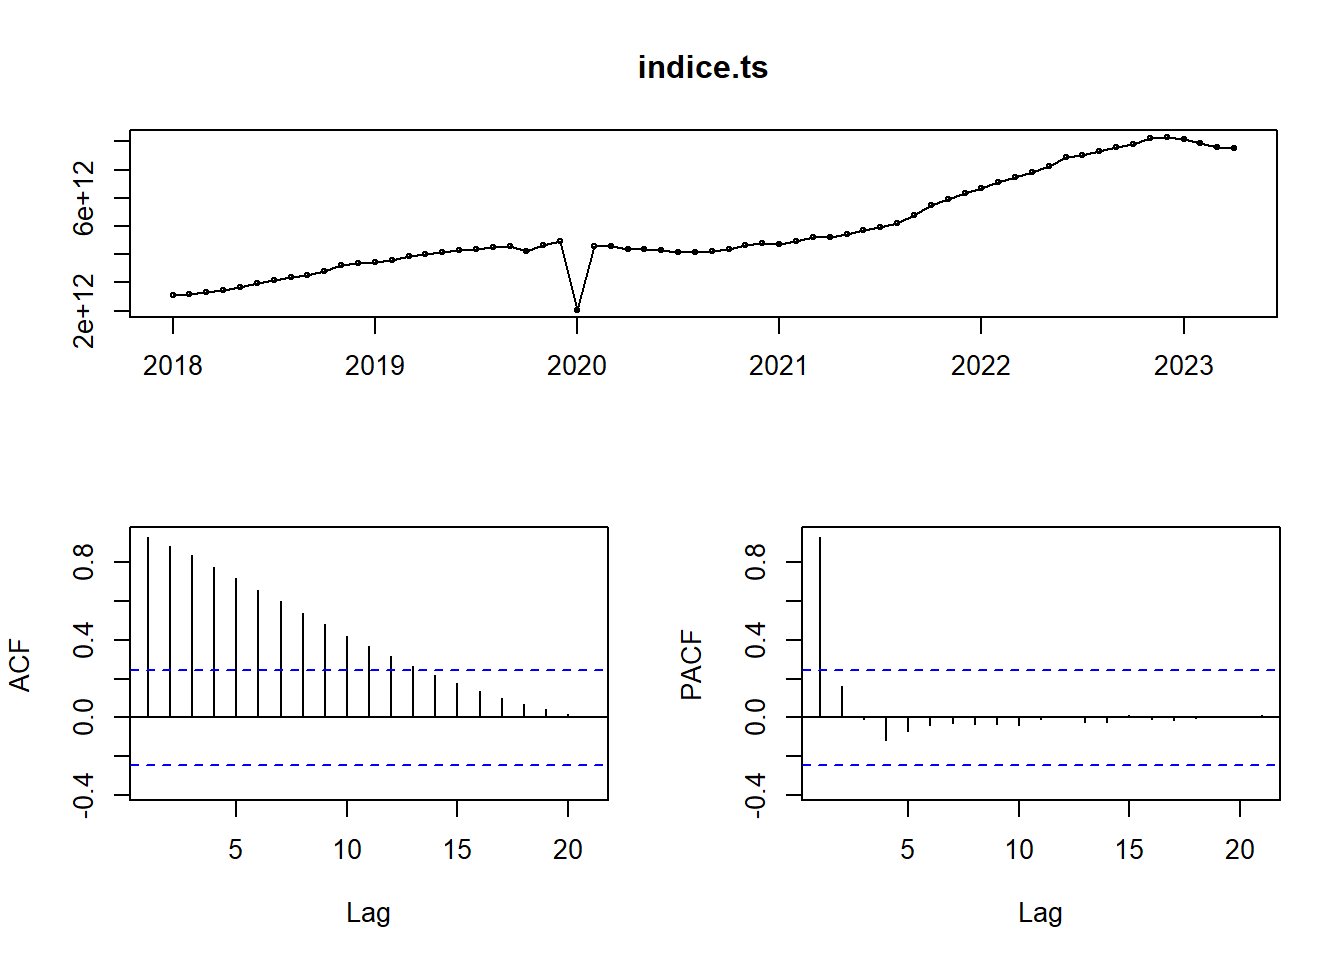
\includegraphics{bookdown-demo_files/figure-latex/unnamed-chunk-24-1.pdf}

Procedemos a diferenciarla ya que es No-Estacionaria
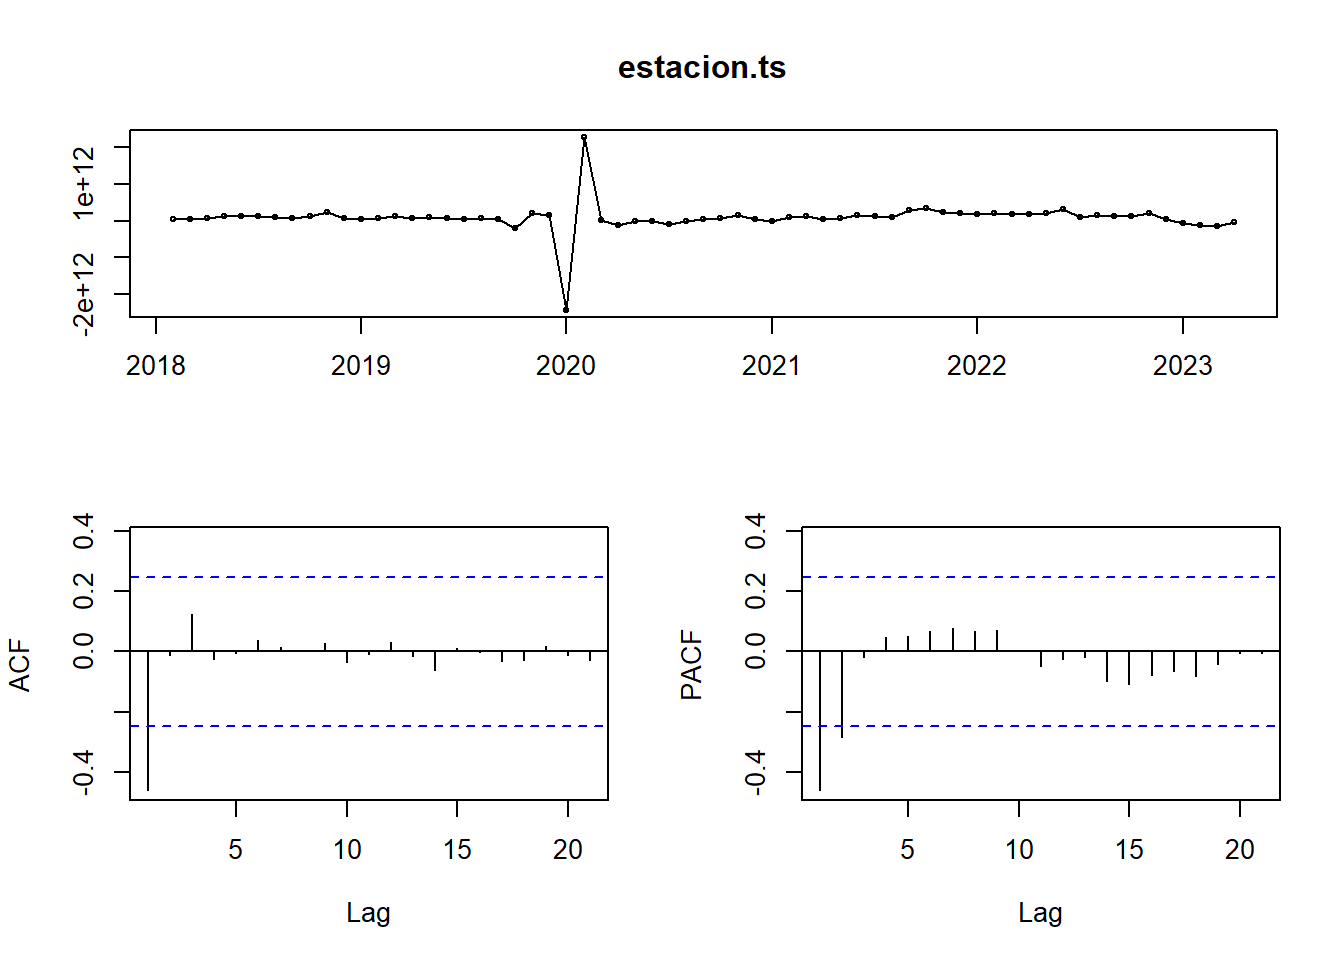
\includegraphics{bookdown-demo_files/figure-latex/unnamed-chunk-25-1.pdf}

\begin{verbatim}
## [1] 0
\end{verbatim}

En el grafico PAFC podemos ver los lag en 1 como punto significativo de cambio.

Construyamos entonces nuestro modelo con valor AR (p) = 1. A tener en cuenta: Al tener un modelo diferenciado, debemos especificar que no se incluya la media en los calculos ya que la misma es 0.

\begin{verbatim}
## 
## Call:
## arima(x = estacion.ts, order = c(1, 0, 0), include.mean = F)
## 
## Coefficients:
##           ar1
##       -0.4010
## s.e.   0.1139
## 
## sigma^2 estimated as 1.621e+23:  log likelihood = -1772.91,  aic = 3549.83
\end{verbatim}

\hypertarget{modelo-basado-solamente-en-el-moving-average-ma.-parametros-p-y-d-en-0}{%
\subsection{Modelo basado solamente en el Moving Average (MA). Parametros p y d en 0}\label{modelo-basado-solamente-en-el-moving-average-ma.-parametros-p-y-d-en-0}}

Utilizando el grafico ACF revisamos cual seria el punto de inflexion y luego procedemos a crear nuestro modelo

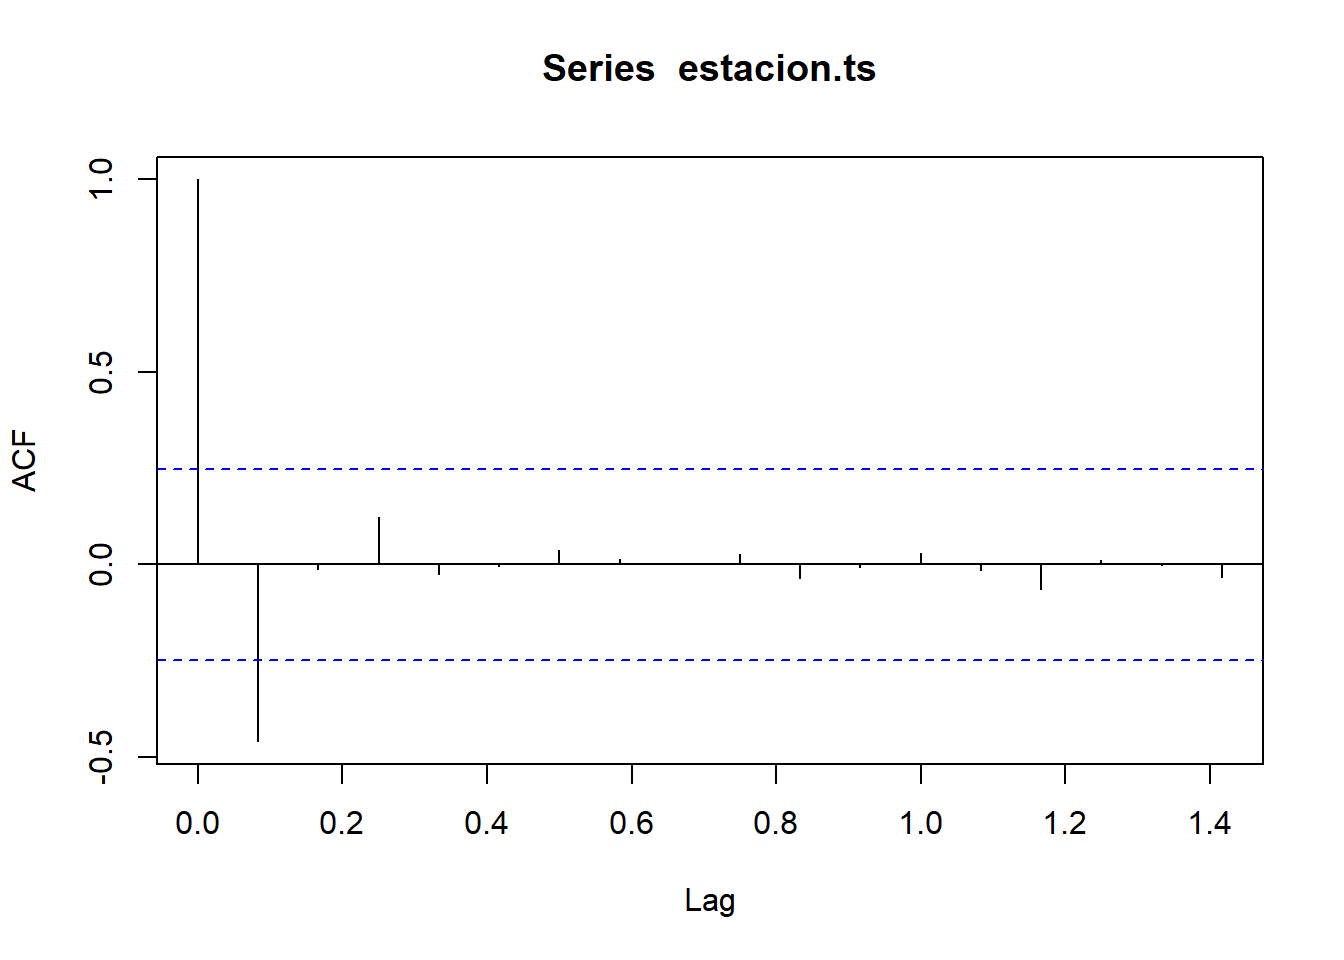
\includegraphics{bookdown-demo_files/figure-latex/unnamed-chunk-27-1.pdf}

\begin{verbatim}
## [1] "Observamos que el 2do lag contiene el ultimo cambio significativo. Ademas el 1ero es descartable siempre ya que es comparable solo consigo mismo."
\end{verbatim}

\begin{verbatim}
## 
## Call:
## arima(x = estacion.ts, order = c(0, 0, 2), include.mean = F)
## 
## Coefficients:
##           ma1     ma2
##       -0.5263  0.2126
## s.e.   0.1412  0.1260
## 
## sigma^2 estimated as 1.556e+23:  log likelihood = -1771.7,  aic = 3549.39
\end{verbatim}

\hypertarget{modelo-arima.-validacion-por-medio-de-la-funcion-auto.arima}{%
\section{Modelo ARIMA. Validacion por medio de la funcion auto.arima}\label{modelo-arima.-validacion-por-medio-de-la-funcion-auto.arima}}

Como pudimos comprobar en los puntos anteriores, la seleccion de parametros del modelo clasico Arima, depende de las caracteristicas de la serie de tiempo a evaluar. Es por ello que decidimos comparar el calculo manual de nuestras variables con respecto al modelo automatico que viene incluido en la libreria de forecast auto.arima.

Para mostrar los resultados, debemos habilitar la opcion trace la cual permite evaluar todos los modelos que pudiesen resultar de la serie de tiempo. Asi mismo, decidimos utilizar 2 parametros mas y configurarlos en Falso - Stepwise y Approximation - los cuales maximizan la busqueda del mejor modelo, al tiempo que sacrifica tanto numero de modelos a evaluar asi como velocidad de respuesta.

\begin{verbatim}
## 
##  ARIMA(0,0,0)            with zero mean     : 3559.137
##  ARIMA(0,0,0)(0,0,1)[12] with zero mean     : 3561.092
##  ARIMA(0,0,0)(1,0,0)[12] with zero mean     : 3561.089
##  ARIMA(0,0,0)(1,0,1)[12] with zero mean     : 3563.321
##  ARIMA(0,0,1)            with zero mean     : 3550.238
##  ARIMA(0,0,1)(0,0,1)[12] with zero mean     : 3551.857
##  ARIMA(0,0,1)(1,0,0)[12] with zero mean     : 3551.834
##  ARIMA(0,0,1)(1,0,1)[12] with zero mean     : Inf
##  ARIMA(0,0,2)            with zero mean     : 3549.801
##  ARIMA(0,0,2)(0,0,1)[12] with zero mean     : 3551.52
##  ARIMA(0,0,2)(1,0,0)[12] with zero mean     : 3551.505
##  ARIMA(0,0,2)(1,0,1)[12] with zero mean     : Inf
##  ARIMA(0,0,3)            with zero mean     : 3549.69
##  ARIMA(0,0,3)(0,0,1)[12] with zero mean     : 3551.74
##  ARIMA(0,0,3)(1,0,0)[12] with zero mean     : 3551.735
##  ARIMA(0,0,3)(1,0,1)[12] with zero mean     : 3554.18
##  ARIMA(0,0,4)            with zero mean     : 3551.745
##  ARIMA(0,0,4)(0,0,1)[12] with zero mean     : 3553.955
##  ARIMA(0,0,4)(1,0,0)[12] with zero mean     : 3553.952
##  ARIMA(0,0,5)            with zero mean     : 3553.08
##  ARIMA(1,0,0)            with zero mean     : 3550.027
##  ARIMA(1,0,0)(0,0,1)[12] with zero mean     : 3551.701
##  ARIMA(1,0,0)(1,0,0)[12] with zero mean     : 3551.685
##  ARIMA(1,0,0)(1,0,1)[12] with zero mean     : Inf
##  ARIMA(1,0,1)            with zero mean     : 3551.278
##  ARIMA(1,0,1)(0,0,1)[12] with zero mean     : 3552.931
##  ARIMA(1,0,1)(1,0,0)[12] with zero mean     : 3552.909
##  ARIMA(1,0,1)(1,0,1)[12] with zero mean     : Inf
##  ARIMA(1,0,2)            with zero mean     : 3544.017
##  ARIMA(1,0,2)(0,0,1)[12] with zero mean     : 3546.351
##  ARIMA(1,0,2)(1,0,0)[12] with zero mean     : 3546.354
##  ARIMA(1,0,2)(1,0,1)[12] with zero mean     : 3548.724
##  ARIMA(1,0,3)            with zero mean     : 3546.198
##  ARIMA(1,0,3)(0,0,1)[12] with zero mean     : 3548.603
##  ARIMA(1,0,3)(1,0,0)[12] with zero mean     : 3548.607
##  ARIMA(1,0,4)            with zero mean     : 3548.636
##  ARIMA(2,0,0)            with zero mean     : 3550.466
##  ARIMA(2,0,0)(0,0,1)[12] with zero mean     : 3552.099
##  ARIMA(2,0,0)(1,0,0)[12] with zero mean     : 3552.075
##  ARIMA(2,0,0)(1,0,1)[12] with zero mean     : Inf
##  ARIMA(2,0,1)            with zero mean     : 3552.408
##  ARIMA(2,0,1)(0,0,1)[12] with zero mean     : 3554.165
##  ARIMA(2,0,1)(1,0,0)[12] with zero mean     : 3554.143
##  ARIMA(2,0,1)(1,0,1)[12] with zero mean     : Inf
##  ARIMA(2,0,2)            with zero mean     : 3546.184
##  ARIMA(2,0,2)(0,0,1)[12] with zero mean     : 3548.584
##  ARIMA(2,0,2)(1,0,0)[12] with zero mean     : 3548.589
##  ARIMA(2,0,3)            with zero mean     : 3548.597
##  ARIMA(3,0,0)            with zero mean     : 3551.834
##  ARIMA(3,0,0)(0,0,1)[12] with zero mean     : 3553.7
##  ARIMA(3,0,0)(1,0,0)[12] with zero mean     : 3553.683
##  ARIMA(3,0,0)(1,0,1)[12] with zero mean     : Inf
##  ARIMA(3,0,1)            with zero mean     : 3548.871
##  ARIMA(3,0,1)(0,0,1)[12] with zero mean     : Inf
##  ARIMA(3,0,1)(1,0,0)[12] with zero mean     : 3551.285
##  ARIMA(3,0,2)            with zero mean     : 3548.575
##  ARIMA(4,0,0)            with zero mean     : 3552.398
##  ARIMA(4,0,0)(0,0,1)[12] with zero mean     : 3554.534
##  ARIMA(4,0,0)(1,0,0)[12] with zero mean     : 3554.529
##  ARIMA(4,0,1)            with zero mean     : 3550.555
##  ARIMA(5,0,0)            with zero mean     : 3553.42
## 
## 
## 
##  Best model: ARIMA(1,0,2)            with zero mean
\end{verbatim}

\begin{verbatim}
## Series: estacion.ts 
## ARIMA(1,0,2) with zero mean 
## 
## Coefficients:
##          ar1      ma1     ma2
##       0.9023  -1.5331  0.6856
## s.e.  0.0701   0.1188  0.1099
## 
## sigma^2 = 1.417e+23:  log likelihood = -1767.66
## AIC=3543.33   AICc=3544.02   BIC=3551.9
\end{verbatim}

Como resultado, podemos concluir que el Modelo ARIMA mas optimo para nuestea serie de datos es el que utiliza un AR = 1, MA = 2 y 0 en su atributo diferenciador.

\hypertarget{analisis}{%
\section{Analisis}\label{analisis}}

\hypertarget{prediccion-del-modelo}{%
\subsection{Prediccion del Modelo}\label{prediccion-del-modelo}}

Utilicemos nuestro modelo ARIMA para pronosticar los siguintes 12 meses de saldo en las cuentas del banco.

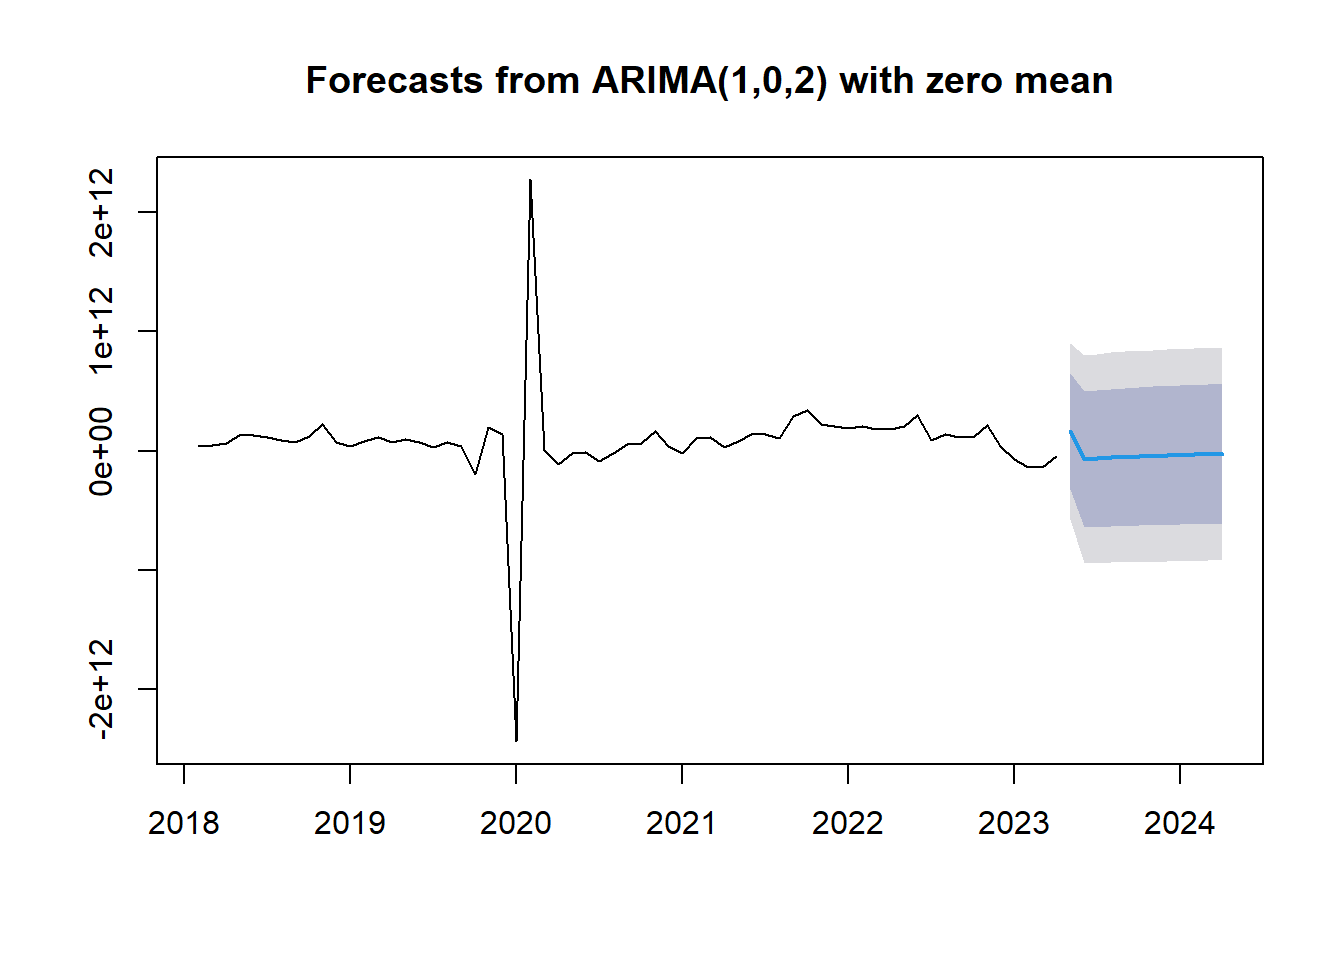
\includegraphics{bookdown-demo_files/figure-latex/unnamed-chunk-29-1.pdf}

\begin{verbatim}
## [1] "Veamos mas en detalle la prediccion de los valores"
\end{verbatim}

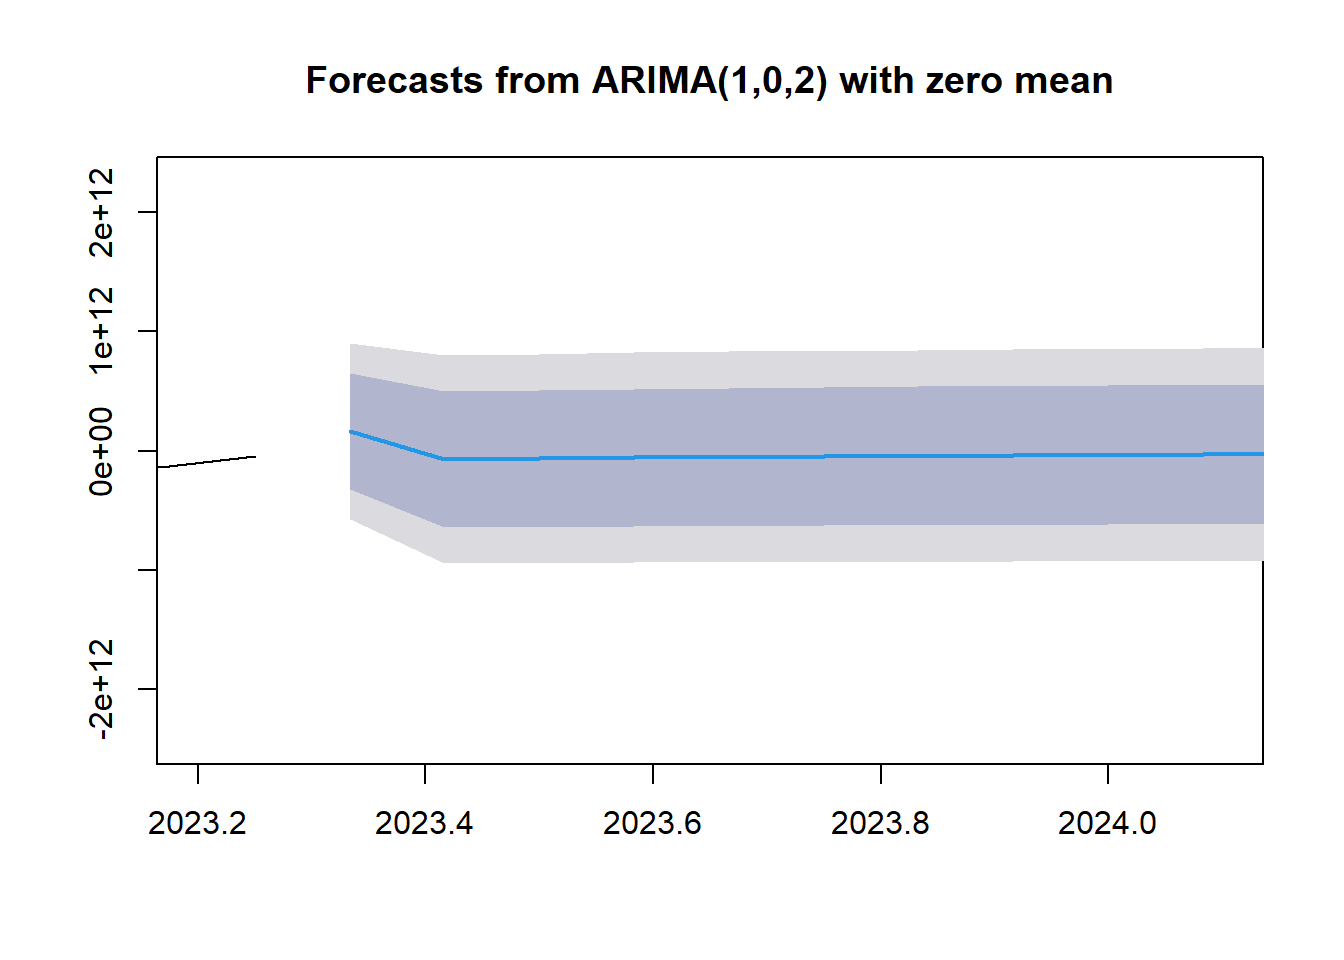
\includegraphics{bookdown-demo_files/figure-latex/unnamed-chunk-29-2.pdf}

\begin{verbatim}
## [1] "Valores de la prediccion:"
\end{verbatim}

\begin{verbatim}
##               Jan          Feb          Mar          Apr          May
## 2023                                                     165668225906
## 2024 -33590498111 -30309584374 -27349130158 -24677834944             
##               Jun          Jul          Aug          Sep          Oct
## 2023 -68971819772 -62235075641 -56156335340 -50671329091 -45722064595
## 2024                                                                 
##               Nov          Dec
## 2023 -41256213885 -37226560069
## 2024
\end{verbatim}

Ahora hagamos las validaciones del modelo

\begin{verbatim}
## [1] "Error in solve.default(res$hessian * n.used, A) :\nLapack routine dgesv: system is exactly singular: U[1,1] = 0"
\end{verbatim}

\begin{verbatim}
## [1] "Al aplicar la funcion tso para encontrar los outliers, nos arroja un error de singularidad, por lo que descarta el uso de diferenciacion para convertir el ts a estacionario."
\end{verbatim}

\hypertarget{diferenciacion-logaritmica}{%
\subsection{Diferenciacion Logaritmica}\label{diferenciacion-logaritmica}}

\begin{Shaded}
\begin{Highlighting}[]
\CommentTok{\# Genero mi objeto ts para el analisis}
\NormalTok{indice.ts }\OtherTok{\textless{}{-}} \FunctionTok{ts}\NormalTok{(datos}\SpecialCharTok{$}\NormalTok{Saldo, }\AttributeTok{start =} \FunctionTok{c}\NormalTok{(}\DecValTok{2018}\NormalTok{,}\DecValTok{1}\NormalTok{), }\AttributeTok{frequency =} \DecValTok{12}\NormalTok{)}
\FunctionTok{plot}\NormalTok{(indice.ts)}
\end{Highlighting}
\end{Shaded}

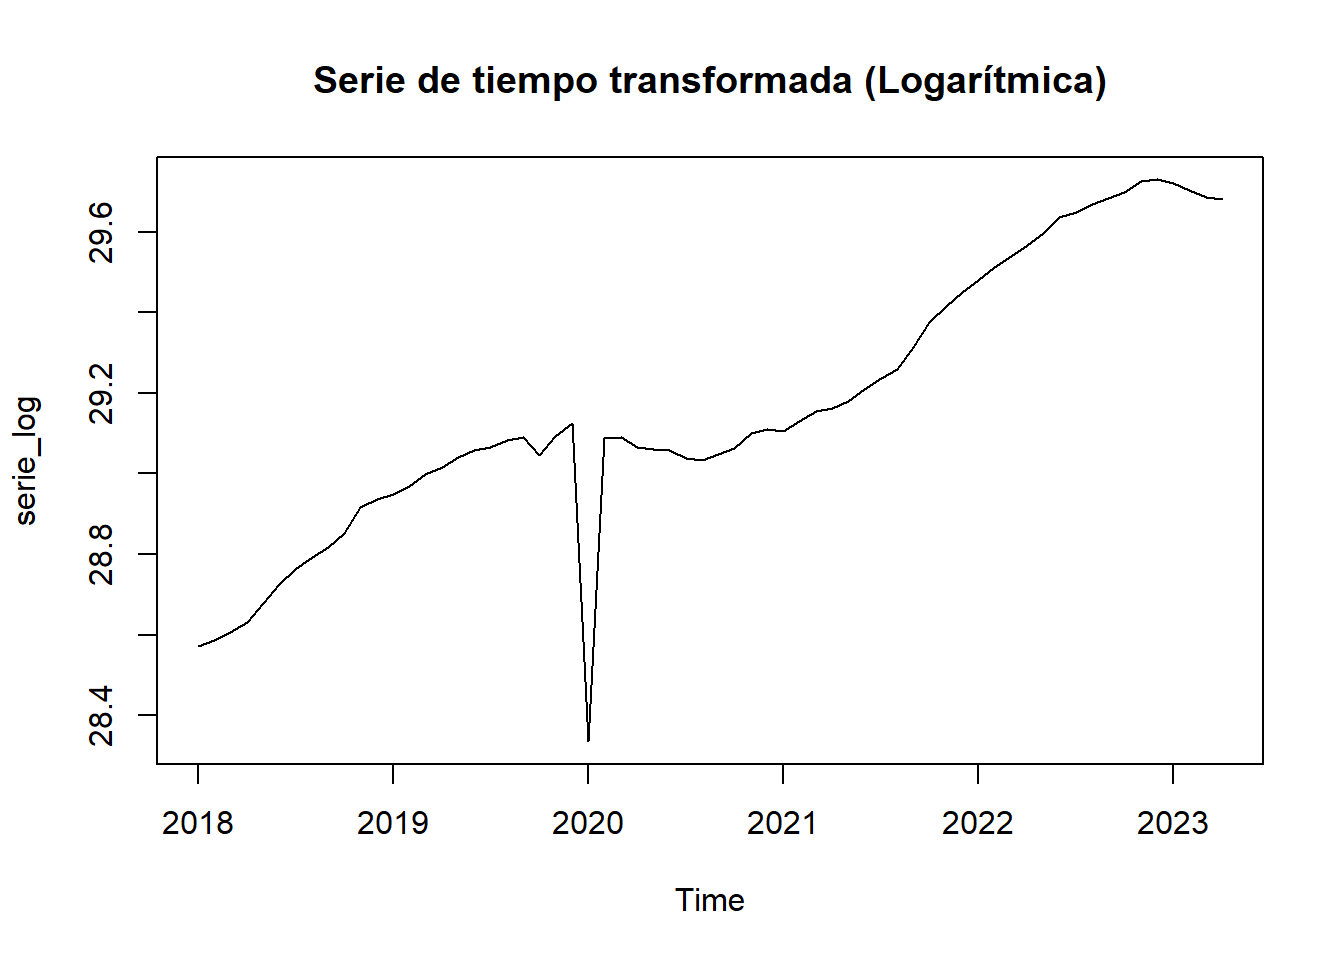
\includegraphics{bookdown-demo_files/figure-latex/unnamed-chunk-31-1.pdf}

\hypertarget{diferenciacion-por-logaritmo}{%
\subsubsection{Diferenciacion por Logaritmo}\label{diferenciacion-por-logaritmo}}

\begin{Shaded}
\begin{Highlighting}[]
\NormalTok{mits }\OtherTok{\textless{}{-}} \FunctionTok{log}\NormalTok{(indice.ts)}

\CommentTok{\# Prueba de Estacionariedad}
\FunctionTok{adf.test}\NormalTok{(mits)}
\end{Highlighting}
\end{Shaded}

\begin{verbatim}
## 
##  Augmented Dickey-Fuller Test
## 
## data:  mits
## Dickey-Fuller = -1.9544, Lag order = 3, p-value = 0.5934
## alternative hypothesis: stationary
\end{verbatim}

\begin{Shaded}
\begin{Highlighting}[]
\FunctionTok{print}\NormalTok{(}\StringTok{"Continua siendo No{-}Estacionaria. Procederemos a diferenciarla"}\NormalTok{)}
\end{Highlighting}
\end{Shaded}

\begin{verbatim}
## [1] "Continua siendo No-Estacionaria. Procederemos a diferenciarla"
\end{verbatim}

\begin{Shaded}
\begin{Highlighting}[]
\NormalTok{mmits }\OtherTok{\textless{}{-}} \FunctionTok{diff}\NormalTok{(mits)}
\FunctionTok{adf.test}\NormalTok{(mmits)}
\end{Highlighting}
\end{Shaded}

\begin{verbatim}
## Warning in adf.test(mmits): p-value smaller than printed p-value
\end{verbatim}

\begin{verbatim}
## 
##  Augmented Dickey-Fuller Test
## 
## data:  mmits
## Dickey-Fuller = -5.3844, Lag order = 3, p-value = 0.01
## alternative hypothesis: stationary
\end{verbatim}

\begin{Shaded}
\begin{Highlighting}[]
\FunctionTok{tsdisplay}\NormalTok{(mmits)}
\end{Highlighting}
\end{Shaded}

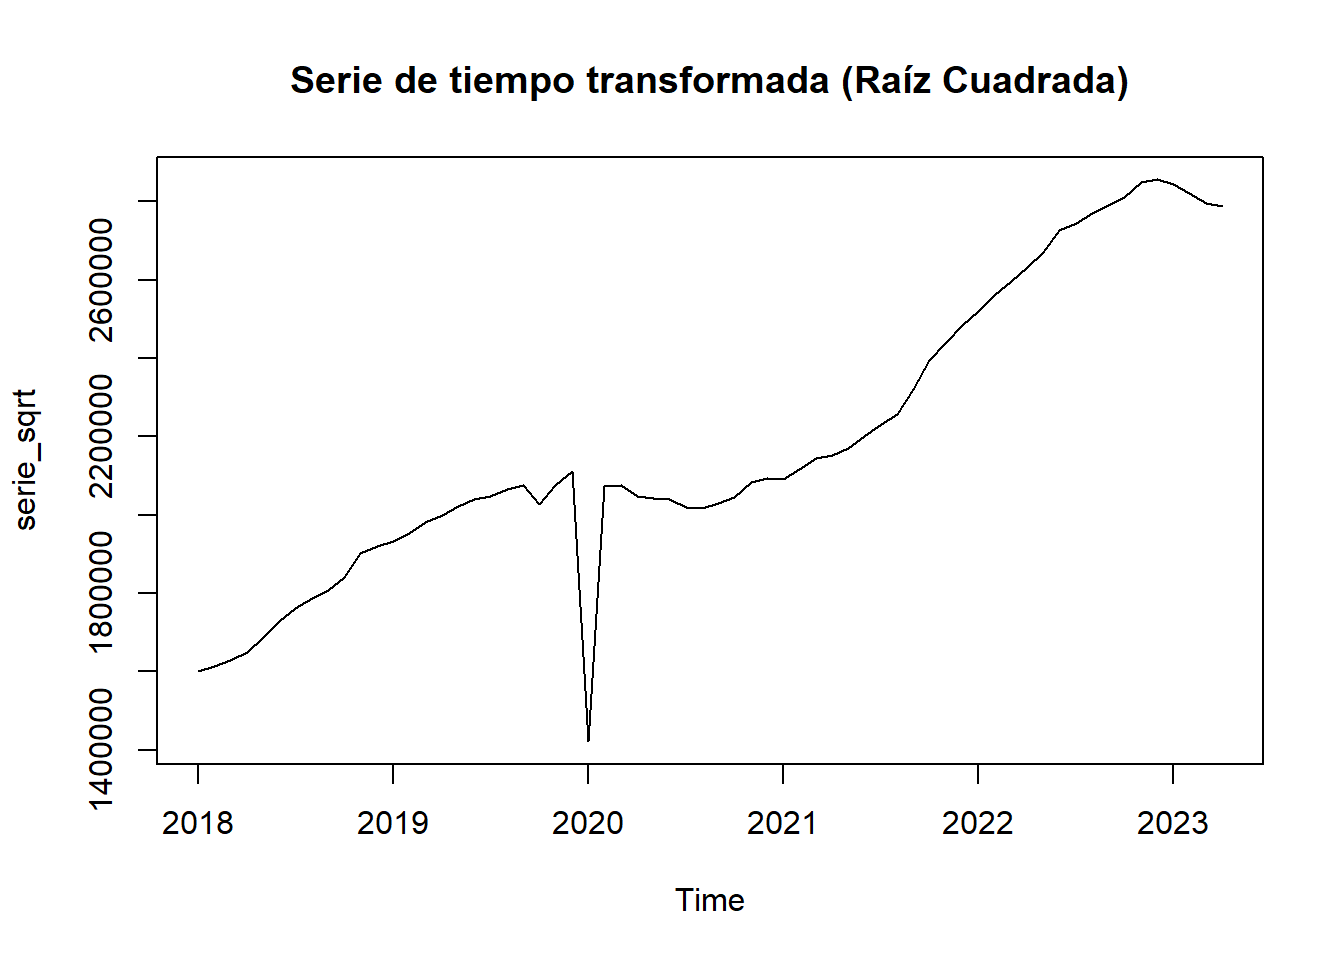
\includegraphics{bookdown-demo_files/figure-latex/unnamed-chunk-32-1.pdf}

\begin{Shaded}
\begin{Highlighting}[]
\FunctionTok{adf.test}\NormalTok{(mmits)}
\end{Highlighting}
\end{Shaded}

\begin{verbatim}
## Warning in adf.test(mmits): p-value smaller than printed p-value
\end{verbatim}

\begin{verbatim}
## 
##  Augmented Dickey-Fuller Test
## 
## data:  mmits
## Dickey-Fuller = -5.3844, Lag order = 3, p-value = 0.01
## alternative hypothesis: stationary
\end{verbatim}

Finalmente podemos recharar la h0 ya que p\textless0.05

\hypertarget{procedamos-a-calular-el-modelo-arima-mas-optimo}{%
\subsubsection{Procedamos a calular el modelo Arima mas optimo:}\label{procedamos-a-calular-el-modelo-arima-mas-optimo}}

\begin{Shaded}
\begin{Highlighting}[]
\NormalTok{mimod }\OtherTok{\textless{}{-}} \FunctionTok{auto.arima}\NormalTok{(mmits, }\AttributeTok{trace =}\NormalTok{ T)}
\end{Highlighting}
\end{Shaded}

\begin{verbatim}
## 
##  ARIMA(2,0,2)(1,0,1)[12] with non-zero mean : Inf
##  ARIMA(0,0,0)            with non-zero mean : -65.53048
##  ARIMA(1,0,0)(1,0,0)[12] with non-zero mean : -78.58046
##  ARIMA(0,0,1)(0,0,1)[12] with non-zero mean : -88.02136
##  ARIMA(0,0,0)            with zero mean     : -66.66478
##  ARIMA(0,0,1)            with non-zero mean : -90.27983
##  ARIMA(0,0,1)(1,0,0)[12] with non-zero mean : -88.01915
##  ARIMA(0,0,1)(1,0,1)[12] with non-zero mean : Inf
##  ARIMA(1,0,1)            with non-zero mean : -88.46913
##  ARIMA(0,0,2)            with non-zero mean : -88.62053
##  ARIMA(1,0,0)            with non-zero mean : -80.81767
##  ARIMA(1,0,2)            with non-zero mean : -86.98859
##  ARIMA(0,0,1)            with zero mean     : -83.77733
## 
##  Best model: ARIMA(0,0,1)            with non-zero mean
\end{verbatim}

\begin{Shaded}
\begin{Highlighting}[]
\NormalTok{mimod}
\end{Highlighting}
\end{Shaded}

\begin{verbatim}
## Series: mmits 
## ARIMA(0,0,1) with non-zero mean 
## 
## Coefficients:
##           ma1    mean
##       -0.6742  0.0182
## s.e.   0.0846  0.0047
## 
## sigma^2 = 0.01291:  log likelihood = 48.34
## AIC=-90.69   AICc=-90.28   BIC=-84.26
\end{verbatim}

\begin{Shaded}
\begin{Highlighting}[]
\CommentTok{\# Hagamos la prediccion de los siguientes 12 meses.}
\NormalTok{mifore }\OtherTok{\textless{}{-}} \FunctionTok{forecast}\NormalTok{(mimod, }\AttributeTok{h=}\DecValTok{12}\NormalTok{)}
\NormalTok{mifore}
\end{Highlighting}
\end{Shaded}

\begin{verbatim}
##          Point Forecast       Lo 80     Hi 80      Lo 95     Hi 95
## May 2023     0.06780752 -0.07779118 0.2134062 -0.1548665 0.2904815
## Jun 2023     0.01815148 -0.15744629 0.1937492 -0.2504021 0.2867051
## Jul 2023     0.01815148 -0.15744629 0.1937492 -0.2504021 0.2867051
## Aug 2023     0.01815148 -0.15744629 0.1937492 -0.2504021 0.2867051
## Sep 2023     0.01815148 -0.15744629 0.1937492 -0.2504021 0.2867051
## Oct 2023     0.01815148 -0.15744629 0.1937492 -0.2504021 0.2867051
## Nov 2023     0.01815148 -0.15744629 0.1937492 -0.2504021 0.2867051
## Dec 2023     0.01815148 -0.15744629 0.1937492 -0.2504021 0.2867051
## Jan 2024     0.01815148 -0.15744629 0.1937492 -0.2504021 0.2867051
## Feb 2024     0.01815148 -0.15744629 0.1937492 -0.2504021 0.2867051
## Mar 2024     0.01815148 -0.15744629 0.1937492 -0.2504021 0.2867051
## Apr 2024     0.01815148 -0.15744629 0.1937492 -0.2504021 0.2867051
\end{verbatim}

\begin{Shaded}
\begin{Highlighting}[]
\FunctionTok{plot}\NormalTok{(mifore)}
\end{Highlighting}
\end{Shaded}

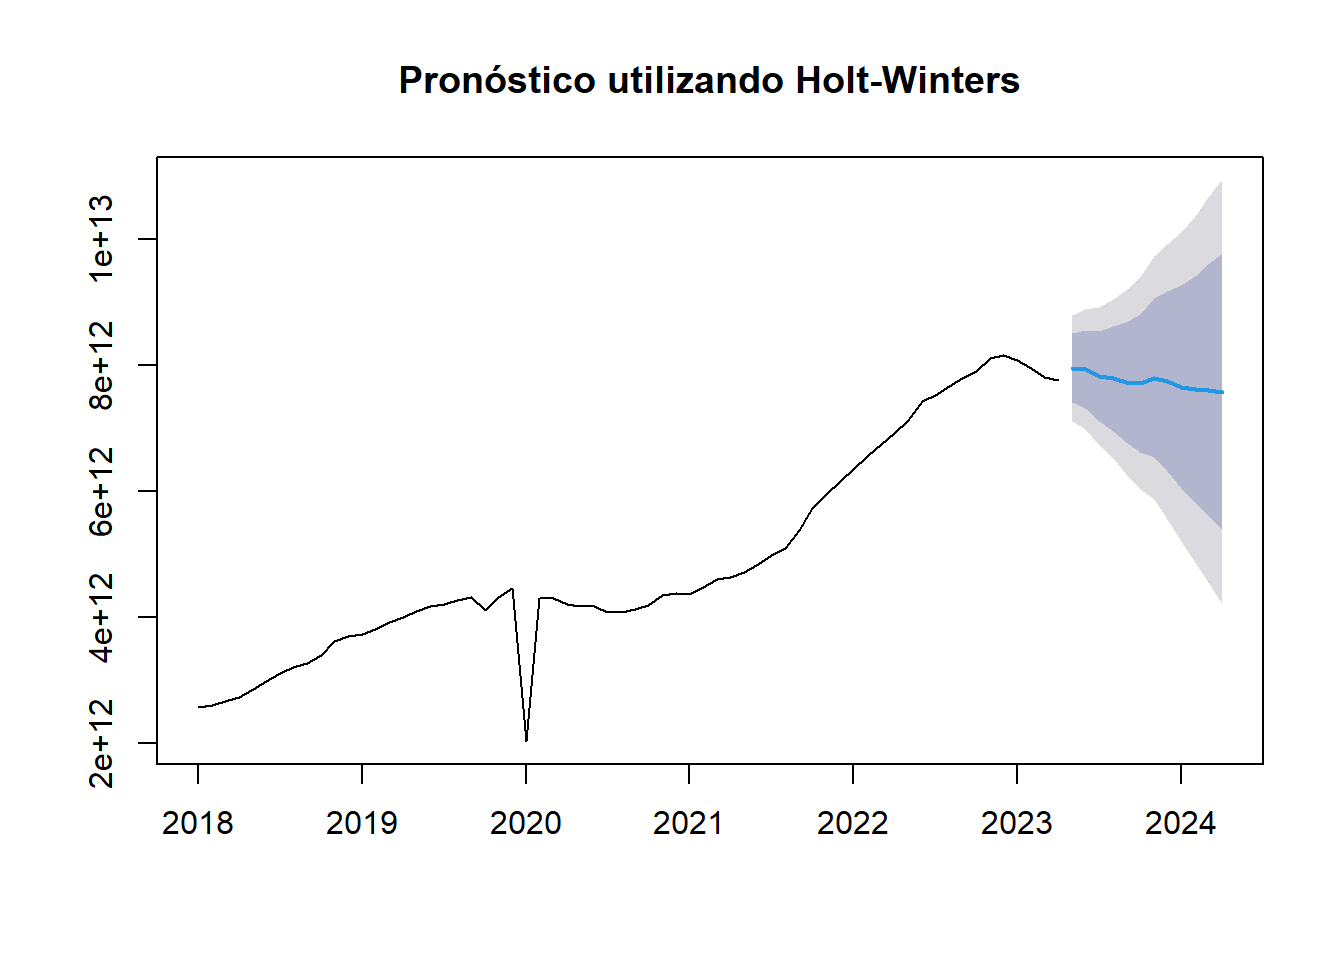
\includegraphics{bookdown-demo_files/figure-latex/unnamed-chunk-33-1.pdf}

\hypertarget{revisemos-el-efecto-de-los-outliers}{%
\subsection{Revisemos el efecto de los outliers:}\label{revisemos-el-efecto-de-los-outliers}}

\begin{Shaded}
\begin{Highlighting}[]
\NormalTok{outliers\_excess\_ts }\OtherTok{\textless{}{-}} \FunctionTok{tso}\NormalTok{(mmits)}
\end{Highlighting}
\end{Shaded}

\begin{verbatim}
## Warning in locate.outliers.iloop(resid = resid, pars = pars, cval = cval, :
## stopped when 'maxit.iloop' was reached

## Warning in locate.outliers.iloop(resid = resid, pars = pars, cval = cval, :
## stopped when 'maxit.iloop' was reached

## Warning in locate.outliers.iloop(resid = resid, pars = pars, cval = cval, :
## stopped when 'maxit.iloop' was reached

## Warning in locate.outliers.iloop(resid = resid, pars = pars, cval = cval, :
## stopped when 'maxit.iloop' was reached
\end{verbatim}

\begin{verbatim}
## Warning in locate.outliers.oloop(y = y, fit = fit, types = types, cval = cval,
## : stopped when 'maxit.oloop = 4' was reached
\end{verbatim}

\begin{Shaded}
\begin{Highlighting}[]
\NormalTok{outliers\_excess\_ts}
\end{Highlighting}
\end{Shaded}

\begin{verbatim}
## Series: mmits 
## Regression with ARIMA(2,0,0) errors 
## 
## Coefficients:
##           ar1      ar2  intercept     TC19    LS20     TC21    AO22     TC23
##       -1.4393  -0.6456     0.0292  -0.0961  0.2422  -0.6172  0.7346  -0.4820
## s.e.   0.0981   0.0953     0.0038   0.0226  0.0286   0.0719  0.0863   0.0285
##         AO25     TC28    LS31     LS35    TC44
##       0.6319  -0.2536  -0.180  -0.0733  0.0521
## s.e.  0.0492   0.0384   0.022   0.0130  0.0145
## 
## sigma^2 = 0.002827:  log likelihood = 101.48
## AIC=-174.96   AICc=-166.21   BIC=-144.96
## 
## Outliers:
##    type ind    time  coefhat   tstat
## 1    TC  19 2019:08 -0.09610  -4.262
## 2    LS  20 2019:09  0.24224   8.461
## 3    TC  21 2019:10 -0.61716  -8.580
## 4    AO  22 2019:11  0.73456   8.516
## 5    TC  23 2019:12 -0.48196 -16.888
## 6    AO  25 2020:02  0.63191  12.842
## 7    TC  28 2020:05 -0.25360  -6.606
## 8    LS  31 2020:08 -0.17998  -8.190
## 9    LS  35 2020:12 -0.07327  -5.620
## 10   TC  44 2021:09  0.05214   3.608
\end{verbatim}

\begin{Shaded}
\begin{Highlighting}[]
\FunctionTok{plot}\NormalTok{(outliers\_excess\_ts)}
\end{Highlighting}
\end{Shaded}

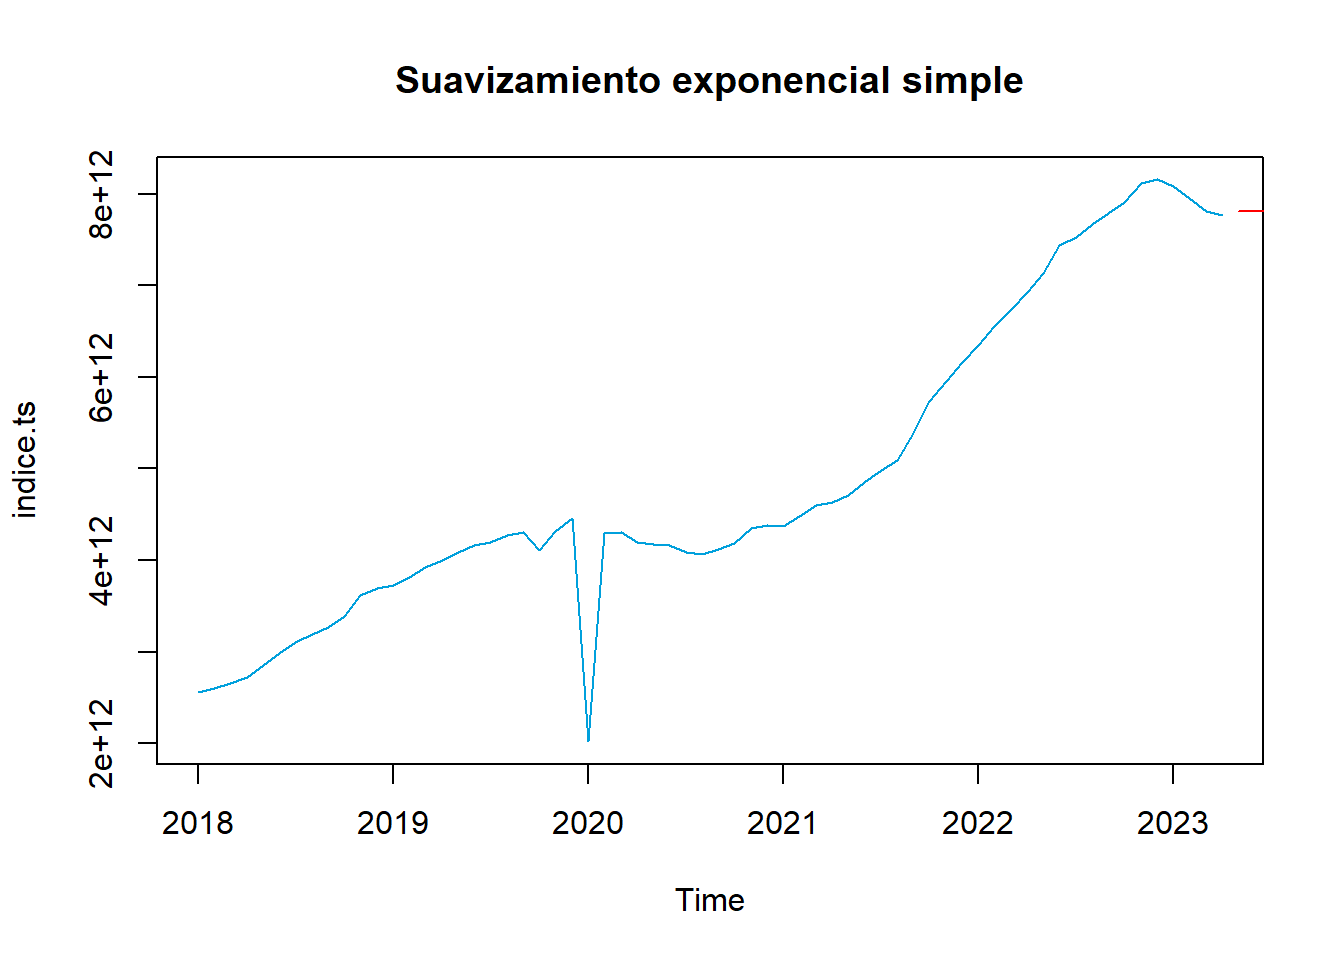
\includegraphics{bookdown-demo_files/figure-latex/unnamed-chunk-34-1.pdf}

La gráfica de Outliers muestra los 10 valores que difieren significativamente del patrón general de la serie de tiempo.

\hypertarget{por-ultimo-haremos-un-check-de-los-residuos.}{%
\subsubsection{Por ultimo haremos un check de los residuos.}\label{por-ultimo-haremos-un-check-de-los-residuos.}}

\begin{Shaded}
\begin{Highlighting}[]
\FunctionTok{checkresiduals}\NormalTok{(mimod)}
\end{Highlighting}
\end{Shaded}

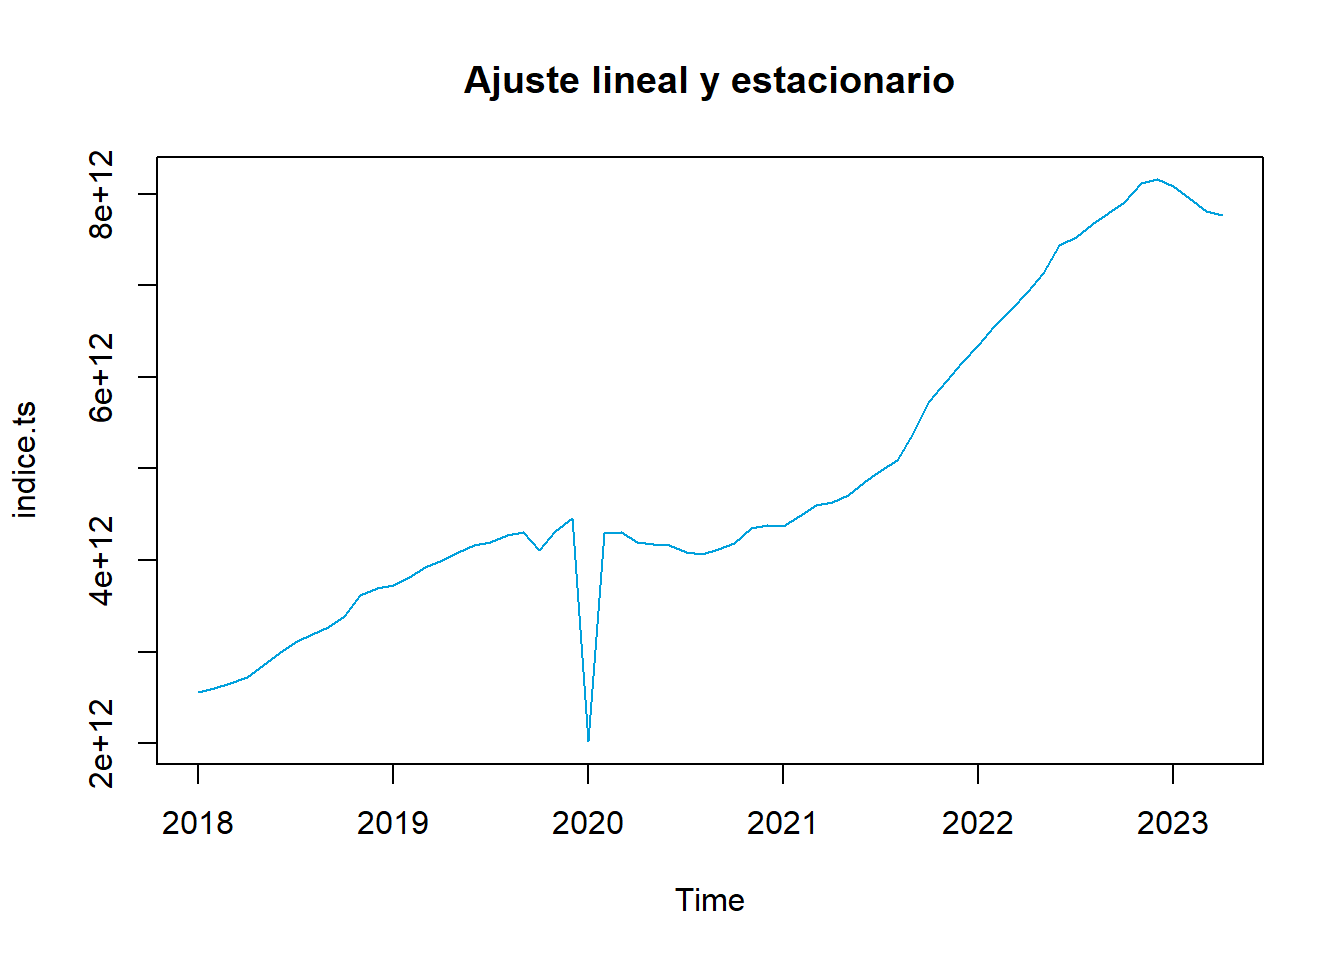
\includegraphics{bookdown-demo_files/figure-latex/unnamed-chunk-35-1.pdf}

\begin{verbatim}
## 
##  Ljung-Box test
## 
## data:  Residuals from ARIMA(0,0,1) with non-zero mean
## Q* = 2.0482, df = 12, p-value = 0.9993
## 
## Model df: 1.   Total lags used: 13
\end{verbatim}

\begin{Shaded}
\begin{Highlighting}[]
\NormalTok{residuales }\OtherTok{\textless{}{-}}\NormalTok{ mimod}\SpecialCharTok{$}\NormalTok{residuals}

\FunctionTok{t.test}\NormalTok{(residuales, }\AttributeTok{alternative=}\StringTok{\textquotesingle{}two.sided\textquotesingle{}}\NormalTok{, }\AttributeTok{conf.level=}\FloatTok{0.95}\NormalTok{, }\AttributeTok{mu=}\DecValTok{0}\NormalTok{)}
\end{Highlighting}
\end{Shaded}

\begin{verbatim}
## 
##  One Sample t-test
## 
## data:  residuales
## t = 0.047608, df = 62, p-value = 0.9622
## alternative hypothesis: true mean is not equal to 0
## 95 percent confidence interval:
##  -0.02770451  0.02905634
## sample estimates:
##    mean of x 
## 0.0006759195
\end{verbatim}

Con esta grafica podemos concluir que los residuales presentan una distribucion normal, que los errores residuales se mantienen dentro del rango de significancia aceptable (0.95) y por medio de un t-test pudimos corroborar que la media de los residuos es 0.

\hypertarget{modelos-logaritmicos-prophet-y-otros}{%
\chapter{Modelos Logaritmicos, Prophet y otros}\label{modelos-logaritmicos-prophet-y-otros}}

\textbf{Transformación logarítmica:}
La transformación logarítmica es útil cuando hay una tendencia exponencial en la serie de tiempo y la varianza aumenta con el nivel de la serie. Aplicar la transformación logarítmica puede ayudar a reducir la tendencia y estabilizar la varianza.se Puede utilizar la función log() para aplicar esta transformación:

\begin{Shaded}
\begin{Highlighting}[]
\CommentTok{\# Aplicar la transformación logarítmica}
\NormalTok{serie\_log }\OtherTok{\textless{}{-}} \FunctionTok{log}\NormalTok{(indice.ts)}

\CommentTok{\# Graficar la serie transformada}
\FunctionTok{plot}\NormalTok{(serie\_log, }\AttributeTok{main =} \StringTok{"Serie de tiempo transformada (Logarítmica)"}\NormalTok{)}
\end{Highlighting}
\end{Shaded}

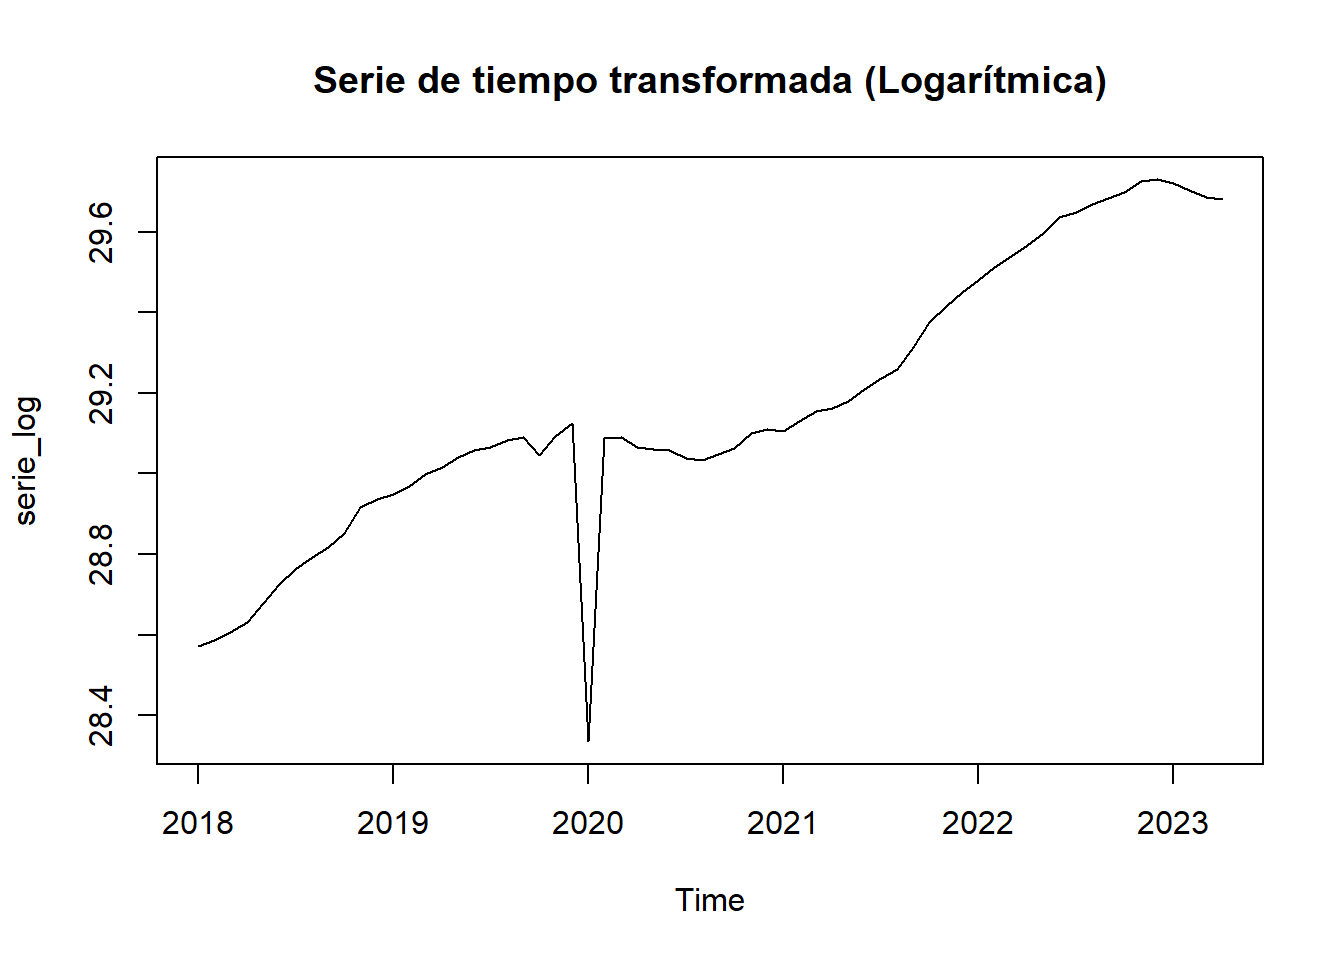
\includegraphics{bookdown-demo_files/figure-latex/unnamed-chunk-36-1.pdf}

\textbf{Transformación de raíz cuadrada:}
La transformación de raíz cuadrada se utiliza cuando la varianza aumenta con el nivel de la serie de tiempo. Al aplicar esta transformación, se reduce la dispersión de los valores más altos y se estabiliza la varianza. Puedes utilizar la función sqrt() para aplicar esta transformación:

\begin{Shaded}
\begin{Highlighting}[]
\CommentTok{\# Aplicar la transformación de raíz cuadrada}
\NormalTok{serie\_sqrt }\OtherTok{\textless{}{-}} \FunctionTok{sqrt}\NormalTok{(indice.ts)}

\CommentTok{\# Graficar la serie transformada}
\FunctionTok{plot}\NormalTok{(serie\_sqrt, }\AttributeTok{main =} \StringTok{"Serie de tiempo transformada (Raíz Cuadrada)"}\NormalTok{)}
\end{Highlighting}
\end{Shaded}

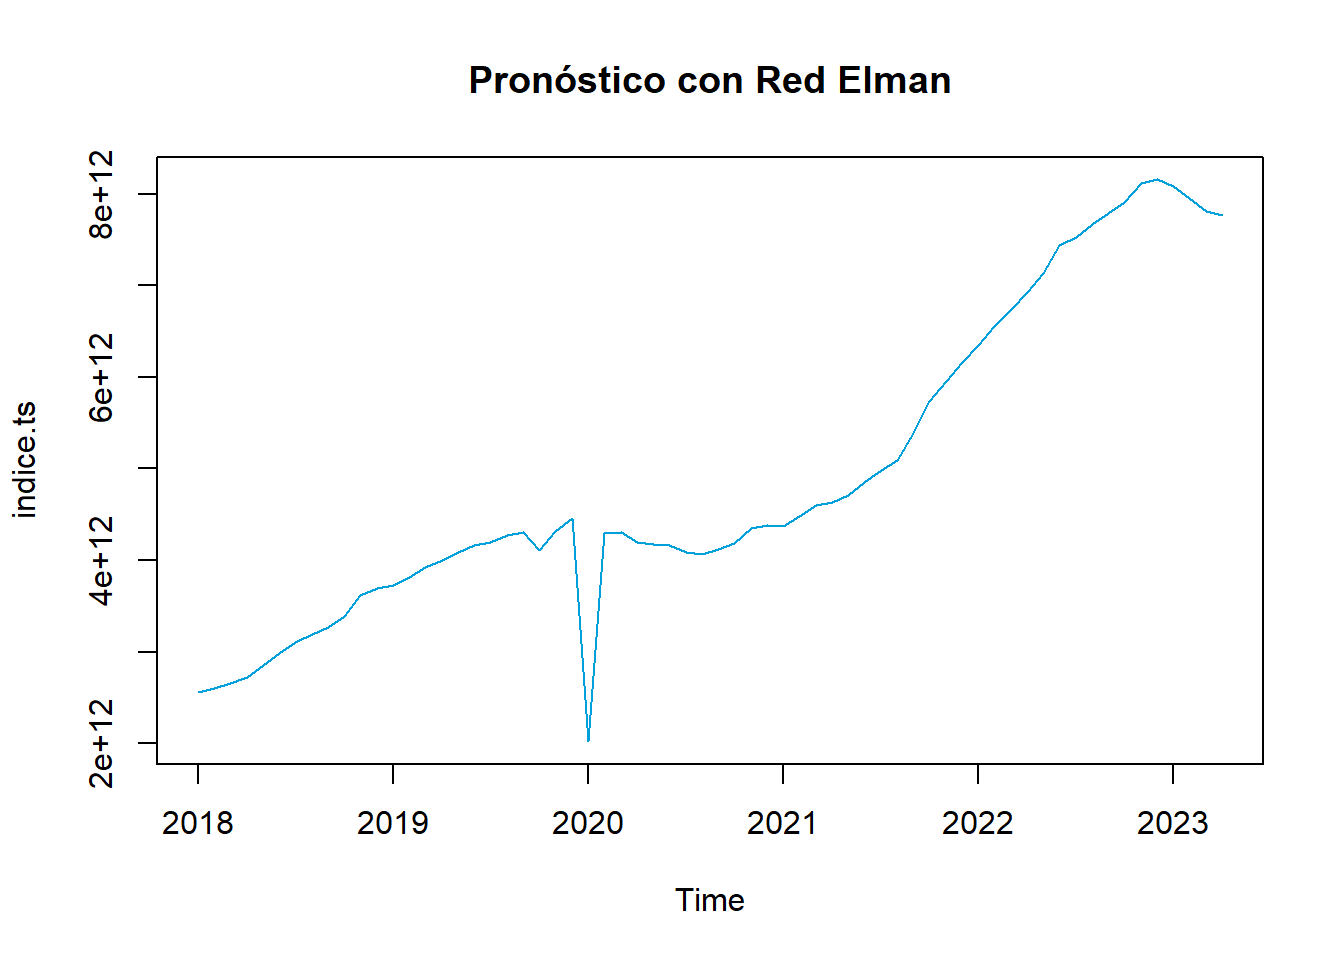
\includegraphics{bookdown-demo_files/figure-latex/unnamed-chunk-37-1.pdf}
Al aplicar estas transformaciones, se espera que la serie de tiempo transformada tenga una tendencia y variabilidad reducidas en comparación con la serie original.

\textbf{Metodología de Holt-Winters:}

Para aplicar la metodología de Holt-Winters y suavizamiento exponencial a la serie de tiempo indice.ts, podemos utilizar las funciones correspondientes de R. La metodología de Holt-Winters es adecuada para modelar series de tiempo con componentes de tendencia y estacionalidad.
El resultado del modelo Holt-Winters proporciona las componentes de tendencia (trend), estacionalidad (seasonal) y residuos (residuals). Estas componentes ayudan a comprender los patrones y la estructura de la serie de tiempo.

\begin{Shaded}
\begin{Highlighting}[]
\FunctionTok{library}\NormalTok{(forecast)}

\CommentTok{\# Aplicar la metodología de Holt{-}Winters}
\NormalTok{hw\_model }\OtherTok{\textless{}{-}} \FunctionTok{HoltWinters}\NormalTok{(indice.ts)}

\CommentTok{\# Obtener el pronóstico utilizando el modelo Holt{-}Winters}
\NormalTok{hw\_forecast }\OtherTok{\textless{}{-}} \FunctionTok{forecast}\NormalTok{(hw\_model, }\AttributeTok{h =} \DecValTok{12}\NormalTok{)  }\CommentTok{\# Pronóstico para los próximos 12 periodos}

\CommentTok{\# Graficar la serie de tiempo y el pronóstico}
\FunctionTok{plot}\NormalTok{(hw\_forecast, }\AttributeTok{main =} \StringTok{"Pronóstico utilizando Holt{-}Winters"}\NormalTok{)}
\end{Highlighting}
\end{Shaded}

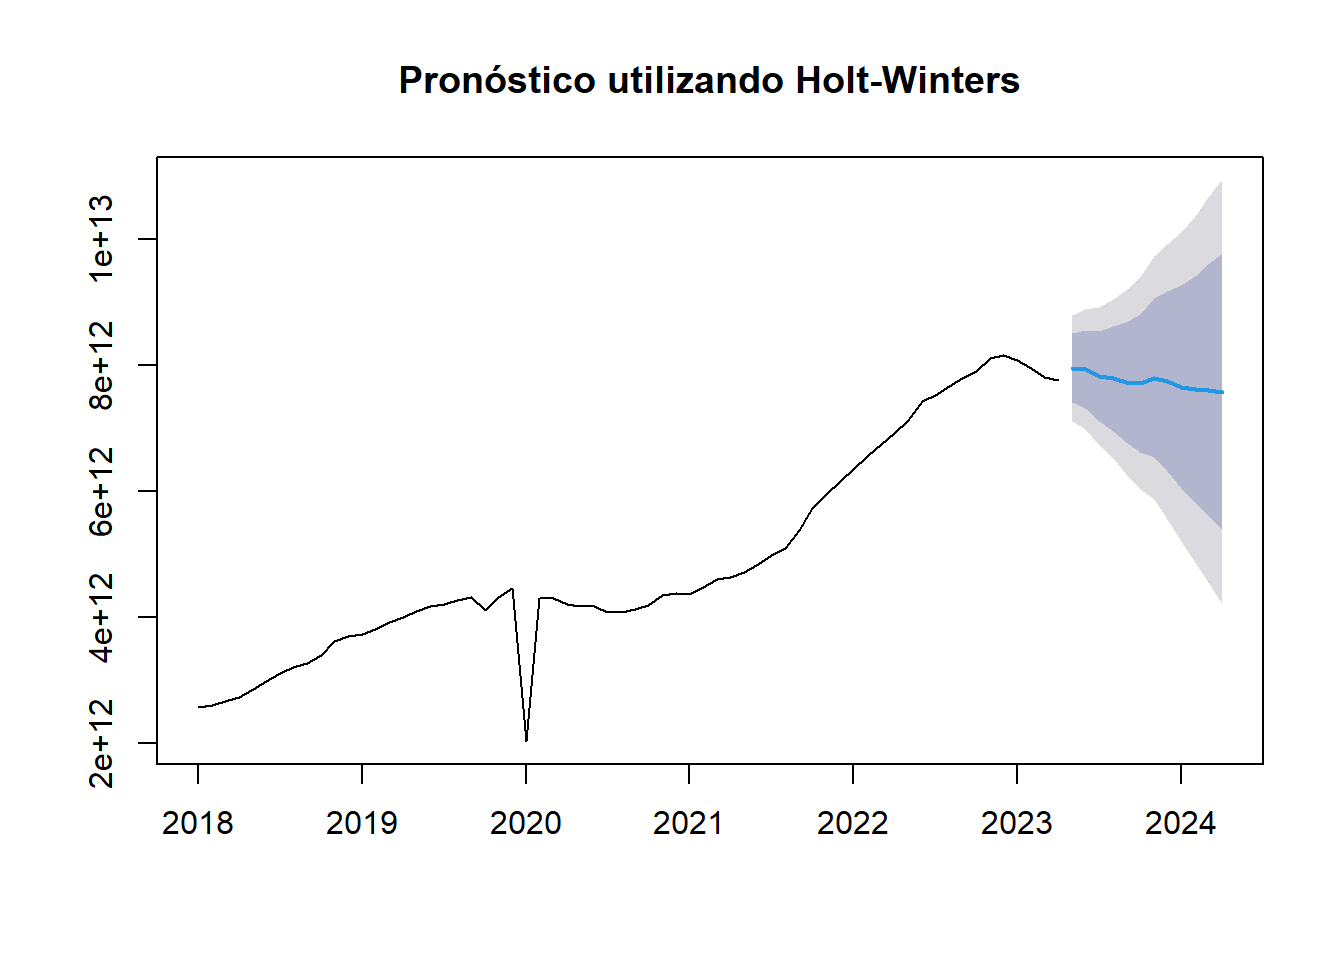
\includegraphics{bookdown-demo_files/figure-latex/unnamed-chunk-38-1.pdf}
Además de la metodología de Holt-Winters, también puedes aplicar técnicas de suavizamiento para obtener una versión suavizada de la serie de tiempo. Una técnica común es el suavizamiento exponencial simple, que calcula un promedio ponderado de los valores anteriores para obtener la versión suavizada de la serie.Se Puede utilizar la función ses() de la librería forecast para aplicar esta técnica:

\begin{Shaded}
\begin{Highlighting}[]
\CommentTok{\# Aplicar suavizamiento exponencial simple}
\NormalTok{ses\_model }\OtherTok{\textless{}{-}} \FunctionTok{ses}\NormalTok{(indice.ts)}

\CommentTok{\# Obtener la serie suavizada}
\NormalTok{horizon }\OtherTok{\textless{}{-}} \DecValTok{6}  \CommentTok{\# Pronosticar 6 períodos hacia adelante}
\NormalTok{ses\_smooth }\OtherTok{\textless{}{-}} \FunctionTok{forecast}\NormalTok{(ses\_model, }\AttributeTok{h =}\NormalTok{ horizon)}\SpecialCharTok{$}\NormalTok{mean}

\CommentTok{\# Graficar la serie de tiempo y la versión suavizada}
\FunctionTok{plot}\NormalTok{(indice.ts, }\AttributeTok{type =} \StringTok{"l"}\NormalTok{, }\AttributeTok{col =} \StringTok{"\#00a0dc"}\NormalTok{, }\AttributeTok{main =} \StringTok{"Suavizamiento exponencial simple"}\NormalTok{)}
\FunctionTok{lines}\NormalTok{(ses\_smooth, }\AttributeTok{col =} \StringTok{"red"}\NormalTok{)}
\end{Highlighting}
\end{Shaded}

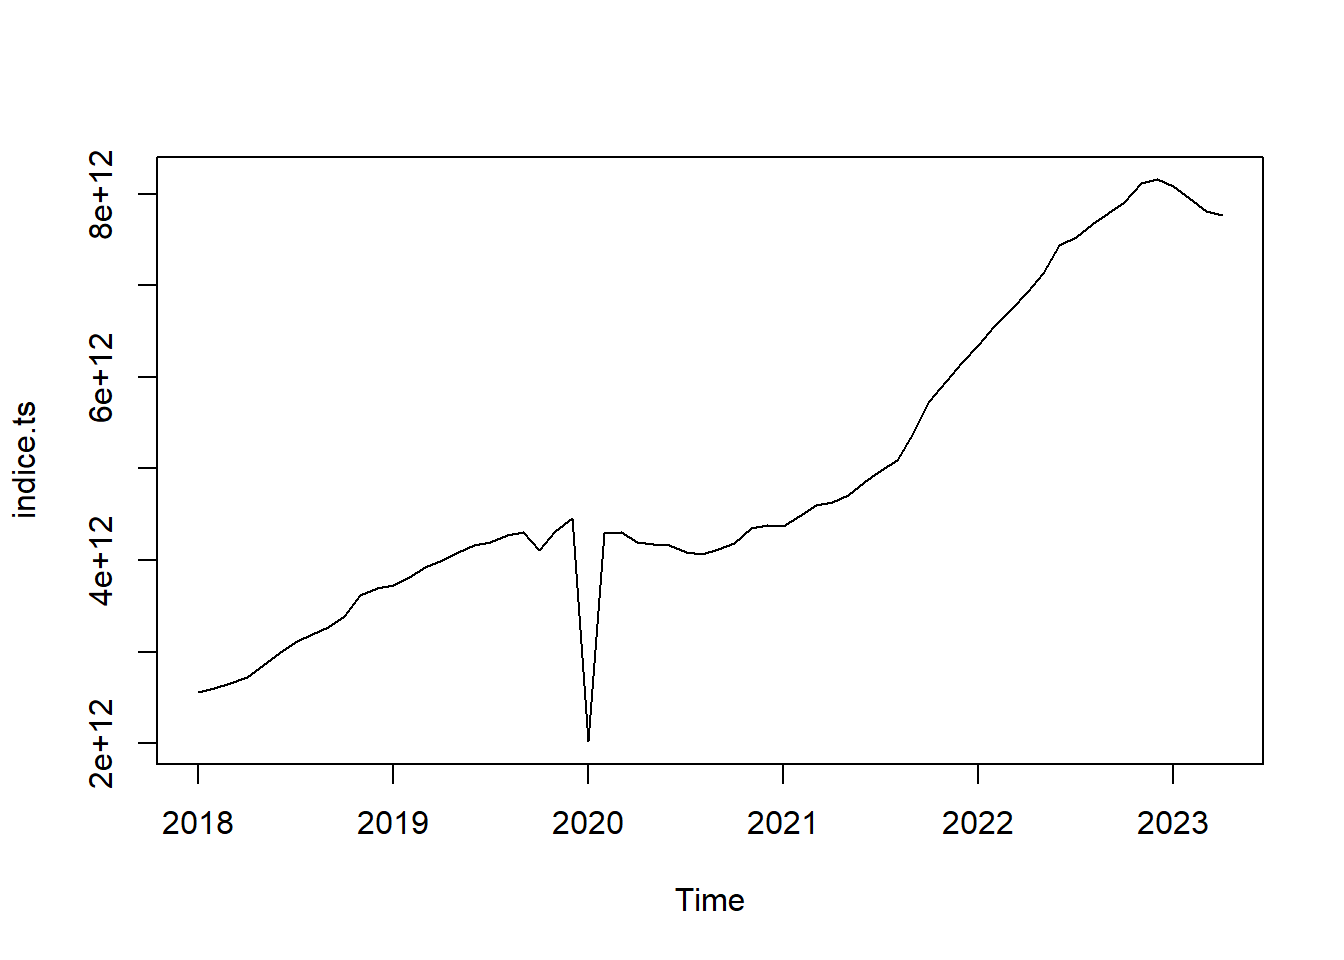
\includegraphics{bookdown-demo_files/figure-latex/unnamed-chunk-39-1.pdf}
El resultado del suavizamiento exponencial simple se muestra en el gráfico que se generó. Aquí hay una explicación de lo que puedes observar en el resultado:

La línea azul representa la serie de tiempo original, es decir, los valores observados de la variable a lo largo del tiempo.
La línea roja representa la versión suavizada de la serie de tiempo, obtenida mediante el suavizamiento exponencial simple.
El suavizamiento exponencial simple utiliza un promedio ponderado de los valores anteriores para generar la versión suavizada. A medida que avanzas en el tiempo, la línea roja muestra una representación suavizada de la tendencia general de la serie.
La versión suavizada ayuda a eliminar el ruido y las fluctuaciones más pequeñas presentes en la serie original. Esto permite visualizar mejor la tendencia subyacente en los datos.
Observa cómo la línea roja se ajusta a la tendencia general de la serie original. En general, el suavizamiento exponencial simple puede ser útil para identificar patrones de tendencia en los datos y proporcionar una representación más clara de la evolución de la variable a lo largo del tiempo.

\textbf{Modelos estacionarios en series de tiempo}

Enfoque de regresión lineal clásico:

\begin{Shaded}
\begin{Highlighting}[]
\CommentTok{\# Crear una variable de tiempo numérica}
\NormalTok{time }\OtherTok{\textless{}{-}} \DecValTok{1}\SpecialCharTok{:}\FunctionTok{length}\NormalTok{(indice.ts)}

\CommentTok{\# Ajustar un modelo lineal y estacionario}
\NormalTok{lm\_model }\OtherTok{\textless{}{-}} \FunctionTok{lm}\NormalTok{(indice.ts }\SpecialCharTok{\textasciitilde{}}\NormalTok{ time)}

\CommentTok{\# Obtener los coeficientes del modelo}
\NormalTok{coef\_lm }\OtherTok{\textless{}{-}} \FunctionTok{coef}\NormalTok{(lm\_model)}

\CommentTok{\# Graficar la serie de tiempo y el modelo ajustado}
\FunctionTok{plot}\NormalTok{(indice.ts, }\AttributeTok{type =} \StringTok{"l"}\NormalTok{, }\AttributeTok{col =} \StringTok{"\#00a0dc"}\NormalTok{, }\AttributeTok{main =} \StringTok{"Ajuste lineal y estacionario"}\NormalTok{)}
\FunctionTok{lines}\NormalTok{(}\FunctionTok{fitted}\NormalTok{(lm\_model), }\AttributeTok{col =} \StringTok{"red"}\NormalTok{)}
\end{Highlighting}
\end{Shaded}

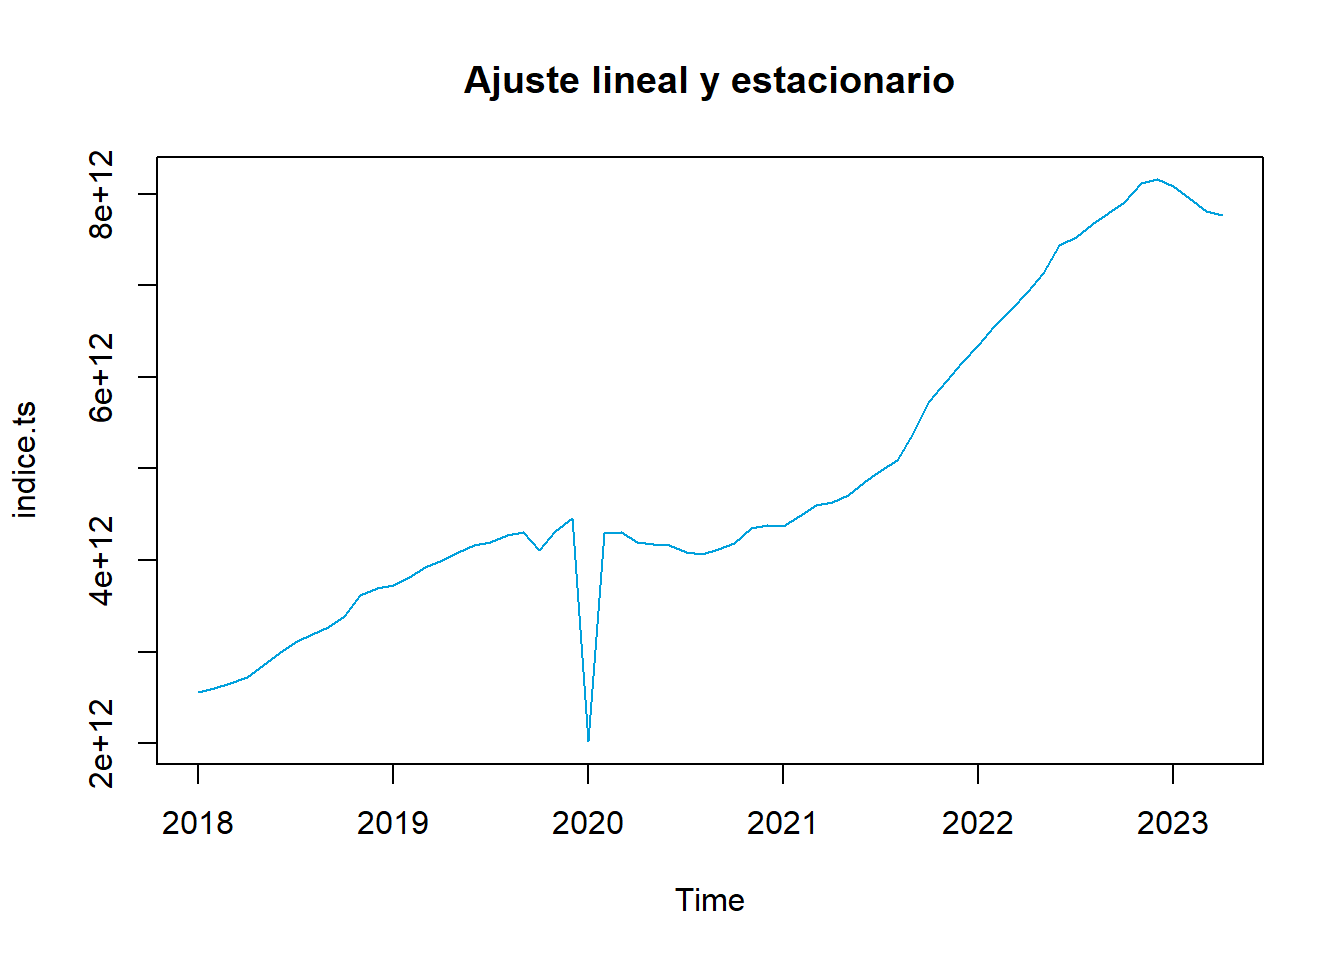
\includegraphics{bookdown-demo_files/figure-latex/unnamed-chunk-40-1.pdf}

\textbf{Algoritmo Facebook´s Prophet:}

\begin{Shaded}
\begin{Highlighting}[]
\CommentTok{\# Instalar y cargar la librería prophet}
\CommentTok{\#install.packages("prophet")}
\FunctionTok{library}\NormalTok{(prophet)}

\CommentTok{\# Crear un dataframe con la serie de tiempo}
\NormalTok{df }\OtherTok{\textless{}{-}} \FunctionTok{data.frame}\NormalTok{(}\AttributeTok{ds =} \FunctionTok{as.Date}\NormalTok{(datos}\SpecialCharTok{$}\NormalTok{Periodo),}
                 \AttributeTok{y =}\NormalTok{ datos}\SpecialCharTok{$}\NormalTok{Saldo)}

\CommentTok{\# Ajustar el modelo Prophet}
\NormalTok{prophet\_model }\OtherTok{\textless{}{-}} \FunctionTok{prophet}\NormalTok{(df)}

\CommentTok{\# Realizar un pronóstico para los próximos 12 meses}
\NormalTok{future }\OtherTok{\textless{}{-}} \FunctionTok{make\_future\_dataframe}\NormalTok{(prophet\_model, }\AttributeTok{periods =} \DecValTok{12}\NormalTok{)}
\NormalTok{forecast }\OtherTok{\textless{}{-}} \FunctionTok{predict}\NormalTok{(prophet\_model, future)}

\CommentTok{\# Graficar el pronóstico}
\FunctionTok{plot}\NormalTok{(prophet\_model, forecast)}
\end{Highlighting}
\end{Shaded}

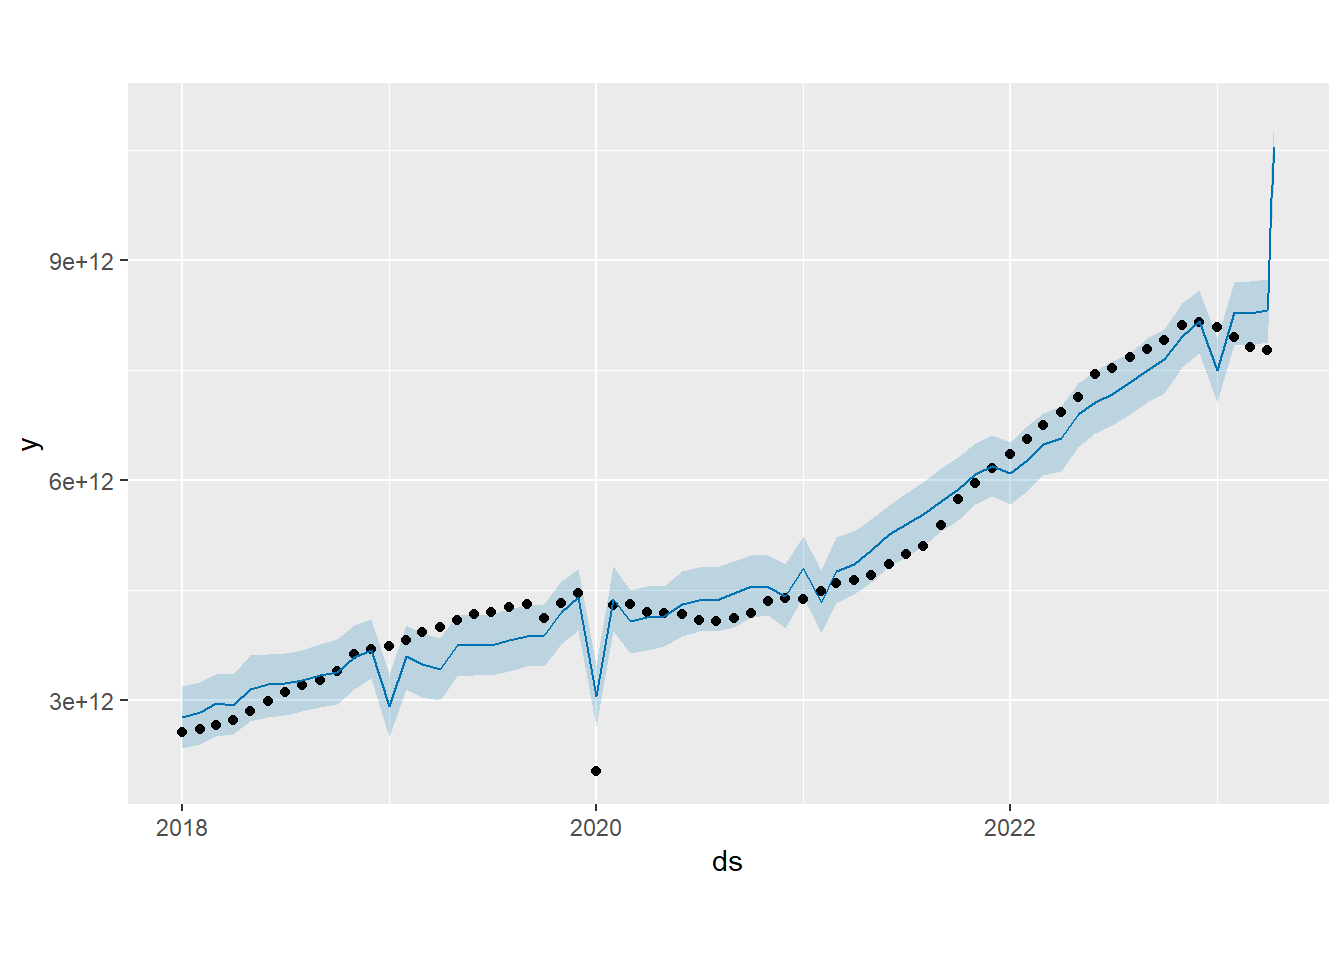
\includegraphics{bookdown-demo_files/figure-latex/unnamed-chunk-41-1.pdf}

\hypertarget{modelos-de-redes-neuronales-recurrentes}{%
\chapter{Modelos de Redes Neuronales Recurrentes}\label{modelos-de-redes-neuronales-recurrentes}}

\hypertarget{elman}{%
\section{Elman}\label{elman}}

Abro la fuente

\begin{Shaded}
\begin{Highlighting}[]
\FunctionTok{library}\NormalTok{(forecast)}
\FunctionTok{library}\NormalTok{(timsac)}
\FunctionTok{library}\NormalTok{(ggplot2)}
\FunctionTok{library}\NormalTok{(changepoint)}
\FunctionTok{library}\NormalTok{(readxl)}
\FunctionTok{library}\NormalTok{(RSNNS)}
\FunctionTok{library}\NormalTok{(quantmod)}
\end{Highlighting}
\end{Shaded}

\begin{verbatim}
## Loading required package: xts
\end{verbatim}

\begin{verbatim}
## Loading required package: TTR
\end{verbatim}

\begin{Shaded}
\begin{Highlighting}[]
\NormalTok{datos }\OtherTok{\textless{}{-}} \FunctionTok{read\_excel}\NormalTok{(}\StringTok{"./fuente/BASE\_Clientes.xlsx"}\NormalTok{)}
\NormalTok{datos}
\end{Highlighting}
\end{Shaded}

\begin{verbatim}
## # A tibble: 643,570 x 8
##    Periodo Sub_Tipo N_Clientes DIAS_DE_MORA     Saldo Genero grupo_actividad_eco
##    <chr>   <chr>         <dbl>        <dbl>     <dbl> <chr>  <chr>              
##  1 2018-01 CDC               4            0 15824105. Femen~ Dependiente privado
##  2 2018-01 CDC               1            0  6810373. Femen~ Dependiente privado
##  3 2018-01 CDC               6            6 28819502. Femen~ Dependiente privado
##  4 2018-01 CDC              12           63 81343674. Femen~ Dependiente privado
##  5 2018-01 CDC               1           21  7524344. Femen~ Dependiente privado
##  6 2018-01 CDC               4            0 12974213. Femen~ Dependiente privado
##  7 2018-01 CDC               3            1 21348609. Femen~ Dependiente privado
##  8 2018-01 CDC               2            0 11475858. Femen~ Dependiente privado
##  9 2018-01 CDC              10           38 60012355. Femen~ Dependiente privado
## 10 2018-01 CDC               1            0  9034715. Femen~ Dependiente privado
## # i 643,560 more rows
## # i 1 more variable: Cuidad_res <chr>
\end{verbatim}

\begin{Shaded}
\begin{Highlighting}[]
\CommentTok{\# Cambio el tipo de dato de la columna temporal(Periodo)}
\NormalTok{datos}\SpecialCharTok{$}\NormalTok{Periodo }\OtherTok{\textless{}{-}} \FunctionTok{as.Date}\NormalTok{(}\FunctionTok{paste0}\NormalTok{(datos}\SpecialCharTok{$}\NormalTok{Periodo, }\StringTok{"{-}01"}\NormalTok{))}

\CommentTok{\# Consolido el df en funcion de la variable de interes (Saldo)}
\NormalTok{datos }\OtherTok{\textless{}{-}} \FunctionTok{aggregate}\NormalTok{(Saldo }\SpecialCharTok{\textasciitilde{}}\NormalTok{ Periodo, }\AttributeTok{data =}\NormalTok{ datos, sum)}

\CommentTok{\# Genero mi objeto ts para el analisis}
\NormalTok{indice.ts }\OtherTok{\textless{}{-}} \FunctionTok{ts}\NormalTok{(datos}\SpecialCharTok{$}\NormalTok{Saldo, }\AttributeTok{start =} \FunctionTok{c}\NormalTok{(}\DecValTok{2018}\NormalTok{,}\DecValTok{1}\NormalTok{), }\AttributeTok{frequency =} \DecValTok{12}\NormalTok{)}
\NormalTok{indice.ts}
\end{Highlighting}
\end{Shaded}

\begin{verbatim}
##               Jan          Feb          Mar          Apr          May
## 2018 2.562223e+12 2.601532e+12 2.653315e+12 2.717915e+12 2.852608e+12
## 2019 3.732137e+12 3.810740e+12 3.923380e+12 3.995810e+12 4.092819e+12
## 2020 2.022405e+12 4.295886e+12 4.304185e+12 4.195404e+12 4.177219e+12
## 2021 4.369300e+12 4.478002e+12 4.595047e+12 4.627874e+12 4.705783e+12
## 2022 6.351501e+12 6.555819e+12 6.739823e+12 6.925001e+12 7.132542e+12
## 2023 8.083445e+12 7.951094e+12 7.812947e+12 7.765132e+12             
##               Jun          Jul          Aug          Sep          Oct
## 2018 2.986446e+12 3.102493e+12 3.196138e+12 3.272388e+12 3.394038e+12
## 2019 4.164386e+12 4.198177e+12 4.267921e+12 4.307340e+12 4.113506e+12
## 2020 4.164434e+12 4.082507e+12 4.067948e+12 4.120926e+12 4.182877e+12
## 2021 4.846473e+12 4.983882e+12 5.091594e+12 5.385784e+12 5.730839e+12
## 2022 7.435792e+12 7.529328e+12 7.670212e+12 7.789046e+12 7.903472e+12
## 2023                                                                 
##               Nov          Dec
## 2018 3.617129e+12 3.690229e+12
## 2019 4.314034e+12 4.455499e+12
## 2020 4.344709e+12 4.384188e+12
## 2021 5.955740e+12 6.164705e+12
## 2022 8.115444e+12 8.154174e+12
## 2023
\end{verbatim}

Ahora convierto mis datos a una time series y luego para el procesamiento de la red neuronal la guardare en una ts normalizada entre 0 y 1

\begin{Shaded}
\begin{Highlighting}[]
\NormalTok{Z }\OtherTok{\textless{}{-}} \FunctionTok{as.ts}\NormalTok{(indice.ts,F)}
\NormalTok{S }\OtherTok{\textless{}{-}}\NormalTok{ (Z}\SpecialCharTok{{-}}\FunctionTok{min}\NormalTok{(Z))}\SpecialCharTok{/}\NormalTok{(}\FunctionTok{max}\NormalTok{(Z)}\SpecialCharTok{{-}}\FunctionTok{min}\NormalTok{(Z))}
\FunctionTok{plot}\NormalTok{(S)}
\end{Highlighting}
\end{Shaded}

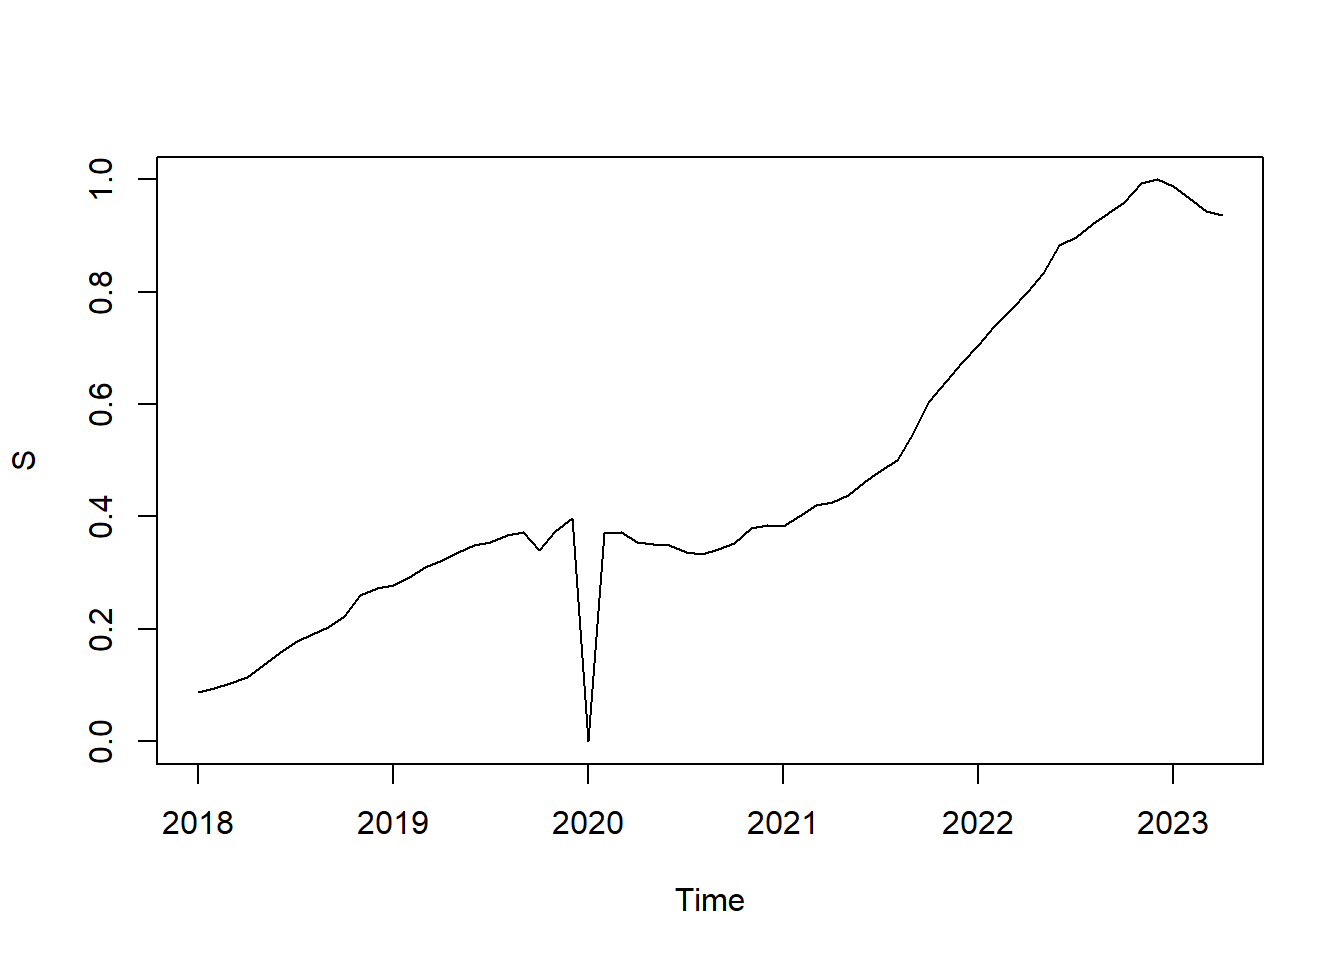
\includegraphics{bookdown-demo_files/figure-latex/unnamed-chunk-43-1.pdf}
Ahora dividiremos el el numero de filas totales

\begin{Shaded}
\begin{Highlighting}[]
\NormalTok{lineas\_totales }\OtherTok{\textless{}{-}}\FunctionTok{length}\NormalTok{(S)}
\NormalTok{t\_train }\OtherTok{\textless{}{-}} \FunctionTok{round}\NormalTok{(lineas\_totales}\SpecialCharTok{*}\FloatTok{0.75}\NormalTok{, }\AttributeTok{digits=}\DecValTok{0}\NormalTok{)}
\NormalTok{l\_train }\OtherTok{\textless{}{-}} \DecValTok{0}\SpecialCharTok{:}\NormalTok{(t\_train}\DecValTok{{-}1}\NormalTok{) }
\NormalTok{t\_test }\OtherTok{\textless{}{-}}\NormalTok{ (t\_train)}\SpecialCharTok{:}\NormalTok{lineas\_totales}
\NormalTok{t\_test}
\end{Highlighting}
\end{Shaded}

\begin{verbatim}
##  [1] 48 49 50 51 52 53 54 55 56 57 58 59 60 61 62 63 64
\end{verbatim}

Ahora crearemos un df cn los nodos que adelantaran un valor en el futuro

\begin{Shaded}
\begin{Highlighting}[]
\NormalTok{y }\OtherTok{\textless{}{-}} \FunctionTok{as.zoo}\NormalTok{(S)}
\NormalTok{x1 }\OtherTok{\textless{}{-}} \FunctionTok{Lag}\NormalTok{(y, }\AttributeTok{k =} \DecValTok{1}\NormalTok{)}
\NormalTok{x2 }\OtherTok{\textless{}{-}} \FunctionTok{Lag}\NormalTok{(y, }\AttributeTok{k =} \DecValTok{2}\NormalTok{)}
\NormalTok{x3 }\OtherTok{\textless{}{-}} \FunctionTok{Lag}\NormalTok{(y, }\AttributeTok{k =} \DecValTok{3}\NormalTok{)}
\NormalTok{x4 }\OtherTok{\textless{}{-}} \FunctionTok{Lag}\NormalTok{(y, }\AttributeTok{k =} \DecValTok{4}\NormalTok{)}
\NormalTok{x5 }\OtherTok{\textless{}{-}} \FunctionTok{Lag}\NormalTok{(y, }\AttributeTok{k =} \DecValTok{5}\NormalTok{)}
\NormalTok{x6 }\OtherTok{\textless{}{-}} \FunctionTok{Lag}\NormalTok{(y, }\AttributeTok{k =} \DecValTok{6}\NormalTok{)}
\NormalTok{x7 }\OtherTok{\textless{}{-}} \FunctionTok{Lag}\NormalTok{(y, }\AttributeTok{k =} \DecValTok{7}\NormalTok{)}
\NormalTok{x8 }\OtherTok{\textless{}{-}} \FunctionTok{Lag}\NormalTok{(y, }\AttributeTok{k =} \DecValTok{8}\NormalTok{)}
\NormalTok{x9 }\OtherTok{\textless{}{-}} \FunctionTok{Lag}\NormalTok{(y, }\AttributeTok{k =} \DecValTok{9}\NormalTok{)}
\NormalTok{x10 }\OtherTok{\textless{}{-}} \FunctionTok{Lag}\NormalTok{(y, }\AttributeTok{k =} \DecValTok{10}\NormalTok{)}
\NormalTok{x11 }\OtherTok{\textless{}{-}} \FunctionTok{Lag}\NormalTok{(y, }\AttributeTok{k =} \DecValTok{11}\NormalTok{)}
\NormalTok{x12 }\OtherTok{\textless{}{-}} \FunctionTok{Lag}\NormalTok{(y, }\AttributeTok{k =} \DecValTok{12}\NormalTok{)}
\NormalTok{slogN }\OtherTok{\textless{}{-}} \FunctionTok{cbind}\NormalTok{(y,x1,x2,x3,x4,x5,x6,x7,x8,x9,x10,x11,x12)}
\CommentTok{\# Elimenemos los valores desplazados}
\NormalTok{slogN }\OtherTok{\textless{}{-}}\NormalTok{ slogN[}\SpecialCharTok{{-}}\NormalTok{(}\DecValTok{1}\SpecialCharTok{:}\DecValTok{12}\NormalTok{),]}
\end{Highlighting}
\end{Shaded}

Acto seguido, especificaremos los inputs y outputs de la red

\begin{Shaded}
\begin{Highlighting}[]
\NormalTok{inputs }\OtherTok{\textless{}{-}}\NormalTok{ slogN[,}\DecValTok{2}\SpecialCharTok{:}\DecValTok{13}\NormalTok{]}
\NormalTok{outputs }\OtherTok{\textless{}{-}}\NormalTok{ slogN[,}\DecValTok{1}\NormalTok{]}
\end{Highlighting}
\end{Shaded}

Con la informaion en su lugar, procedamos a crear la red de Elman

\begin{Shaded}
\begin{Highlighting}[]
\FunctionTok{set.seed}\NormalTok{(}\DecValTok{44}\NormalTok{)}
\NormalTok{fit }\OtherTok{\textless{}{-}}\NormalTok{ fit}\OtherTok{\textless{}{-}}\FunctionTok{elman}\NormalTok{(inputs[t\_train],outputs[t\_train],}\AttributeTok{size=}\FunctionTok{c}\NormalTok{(}\DecValTok{7}\NormalTok{,}\DecValTok{3}\NormalTok{),}\AttributeTok{learnFuncParams=}\FunctionTok{c}\NormalTok{(}\FloatTok{0.1}\NormalTok{),}\AttributeTok{maxit=}\DecValTok{1000}\NormalTok{)}
\end{Highlighting}
\end{Shaded}

Veamos como evoluciona el error

\begin{Shaded}
\begin{Highlighting}[]
\FunctionTok{plotIterativeError}\NormalTok{(fit, }\AttributeTok{main =} \StringTok{"Iterative Error for 7,3 NeuronError Iterativo para neuronas 7,3"}\NormalTok{)}
\end{Highlighting}
\end{Shaded}

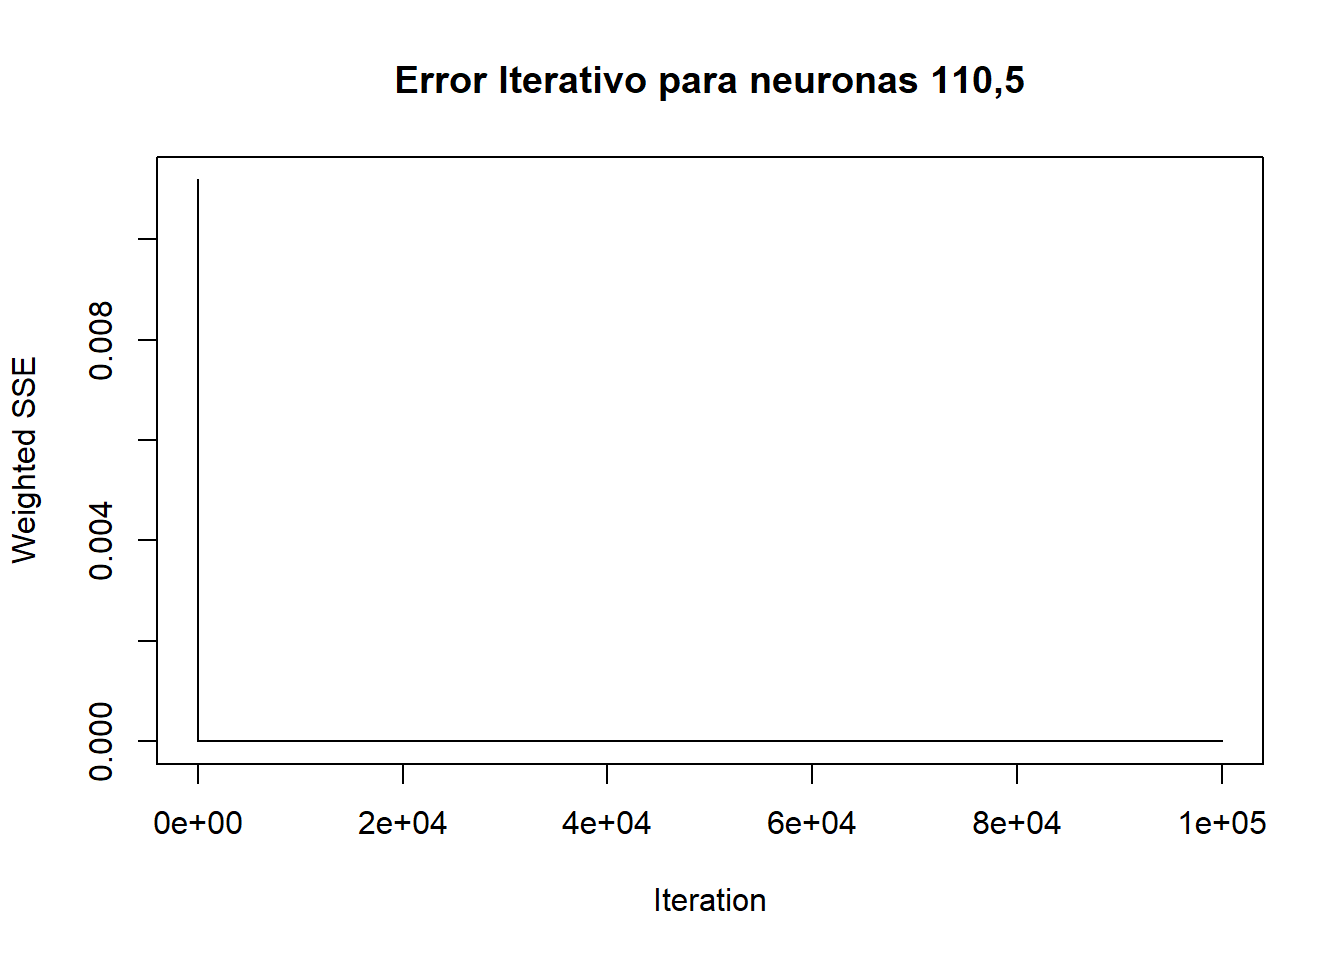
\includegraphics{bookdown-demo_files/figure-latex/unnamed-chunk-48-1.pdf}
Asi podemos ver que el error converge extremadamente rapido

Ahora procederemos a hacer la la pred con el resto de terminosde la seria

\begin{Shaded}
\begin{Highlighting}[]
\NormalTok{y }\OtherTok{\textless{}{-}} \FunctionTok{as.vector}\NormalTok{(outputs[}\SpecialCharTok{{-}}\NormalTok{t\_test])}
\FunctionTok{plot}\NormalTok{(y,}\AttributeTok{type=}\StringTok{"l"}\NormalTok{)}
\NormalTok{pred }\OtherTok{\textless{}{-}} \FunctionTok{predict}\NormalTok{(fit, inputs[}\SpecialCharTok{{-}}\NormalTok{t\_test])}
\FunctionTok{lines}\NormalTok{(pred,}\AttributeTok{col =} \StringTok{"red"}\NormalTok{)}
\end{Highlighting}
\end{Shaded}

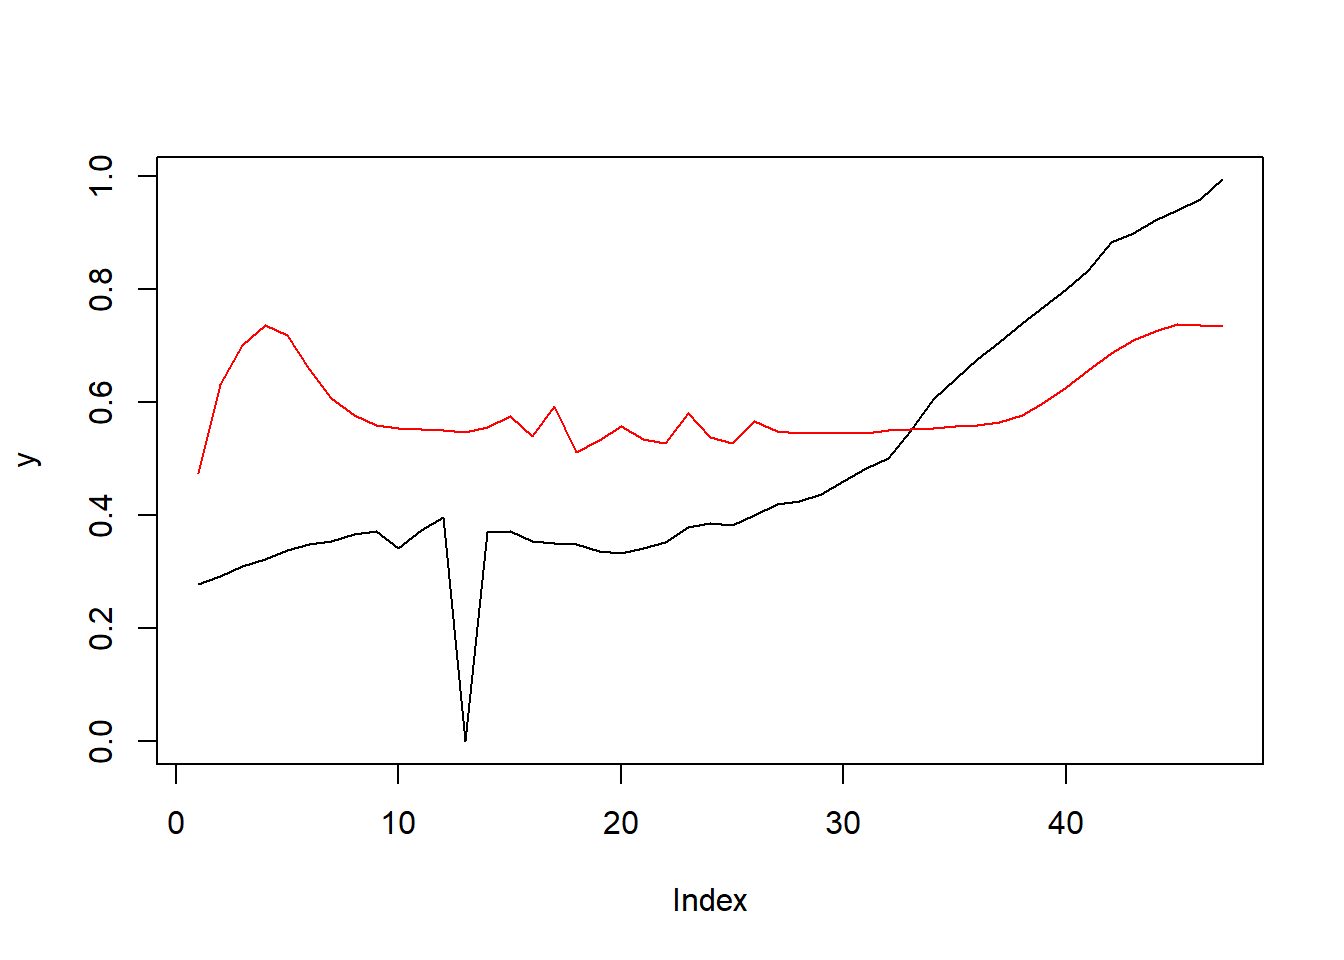
\includegraphics{bookdown-demo_files/figure-latex/unnamed-chunk-49-1.pdf}
ahora predicciones

\begin{Shaded}
\begin{Highlighting}[]
\NormalTok{predictions }\OtherTok{\textless{}{-}} \FunctionTok{predict}\NormalTok{(fit,inputs[}\SpecialCharTok{{-}}\NormalTok{t\_train])}
\end{Highlighting}
\end{Shaded}

desnormalizamos datos

\begin{Shaded}
\begin{Highlighting}[]
\NormalTok{mod5 }\OtherTok{\textless{}{-}}\NormalTok{ predictions}\SpecialCharTok{*}\NormalTok{(}\FunctionTok{max}\NormalTok{(Z)}\SpecialCharTok{{-}}\FunctionTok{min}\NormalTok{(Z))}\SpecialCharTok{+}\FunctionTok{min}\NormalTok{(Z)}
\NormalTok{mod5}
\end{Highlighting}
\end{Shaded}

\begin{verbatim}
##                  [,1]
## Jan 2019 7.479485e+12
## Feb 2019 7.740388e+12
## Mar 2019 7.873136e+12
## Apr 2019 7.928784e+12
## May 2019 7.941933e+12
## Jun 2019 7.943447e+12
## Jul 2019 7.948358e+12
## Aug 2019 7.945146e+12
## Sep 2019 7.939442e+12
## Oct 2019 7.937759e+12
## Nov 2019 7.920444e+12
## Dec 2019 7.907079e+12
## Jan 2020 7.936890e+12
## Feb 2020 7.831769e+12
## Mar 2020 7.738073e+12
## Apr 2020 8.019925e+12
## May 2020 7.972166e+12
## Jun 2020 7.923414e+12
## Jul 2020 7.970784e+12
## Aug 2020 7.867600e+12
## Sep 2020 7.793710e+12
## Oct 2020 7.860149e+12
## Nov 2020 7.885598e+12
## Dec 2020 7.920199e+12
## Jan 2021 8.008120e+12
## Feb 2021 7.961386e+12
## Mar 2021 7.909667e+12
## Apr 2021 7.910477e+12
## May 2021 7.914930e+12
## Jun 2021 7.920344e+12
## Jul 2021 7.939212e+12
## Aug 2021 7.952321e+12
## Sep 2021 7.956209e+12
## Oct 2021 7.965167e+12
## Nov 2021 7.983909e+12
## Dec 2021 7.994656e+12
## Jan 2022 7.995008e+12
## Feb 2022 7.991864e+12
## Mar 2022 7.984059e+12
## Apr 2022 7.983623e+12
## May 2022 7.990518e+12
## Jun 2022 7.996664e+12
## Jul 2022 8.005999e+12
## Aug 2022 8.011570e+12
## Sep 2022 7.995227e+12
## Oct 2022 7.984048e+12
## Nov 2022 7.973629e+12
## Jan 2023 7.978833e+12
## Feb 2023 7.965210e+12
## Mar 2023 7.950325e+12
## Apr 2023 7.941412e+12
\end{verbatim}

veamos los valores

\begin{Shaded}
\begin{Highlighting}[]
\NormalTok{x }\OtherTok{\textless{}{-}} \DecValTok{1}\SpecialCharTok{:}\NormalTok{(lineas\_totales}\SpecialCharTok{+}\FunctionTok{length}\NormalTok{(mod5))}
\NormalTok{y }\OtherTok{\textless{}{-}} \FunctionTok{c}\NormalTok{(}\FunctionTok{as.vector}\NormalTok{(Z),mod5)}
\FunctionTok{plot}\NormalTok{(x[}\DecValTok{1}\SpecialCharTok{:}\NormalTok{lineas\_totales], y[}\DecValTok{1}\SpecialCharTok{:}\NormalTok{lineas\_totales],}\AttributeTok{col =} \StringTok{"blue"}\NormalTok{, }\AttributeTok{type=}\StringTok{"l"}\NormalTok{)}
\FunctionTok{lines}\NormalTok{( x[(lineas\_totales)}\SpecialCharTok{:}\FunctionTok{length}\NormalTok{(x)], y[(lineas\_totales)}\SpecialCharTok{:}\FunctionTok{length}\NormalTok{(x)], }\AttributeTok{col=}\StringTok{"red"}\NormalTok{)}
\end{Highlighting}
\end{Shaded}

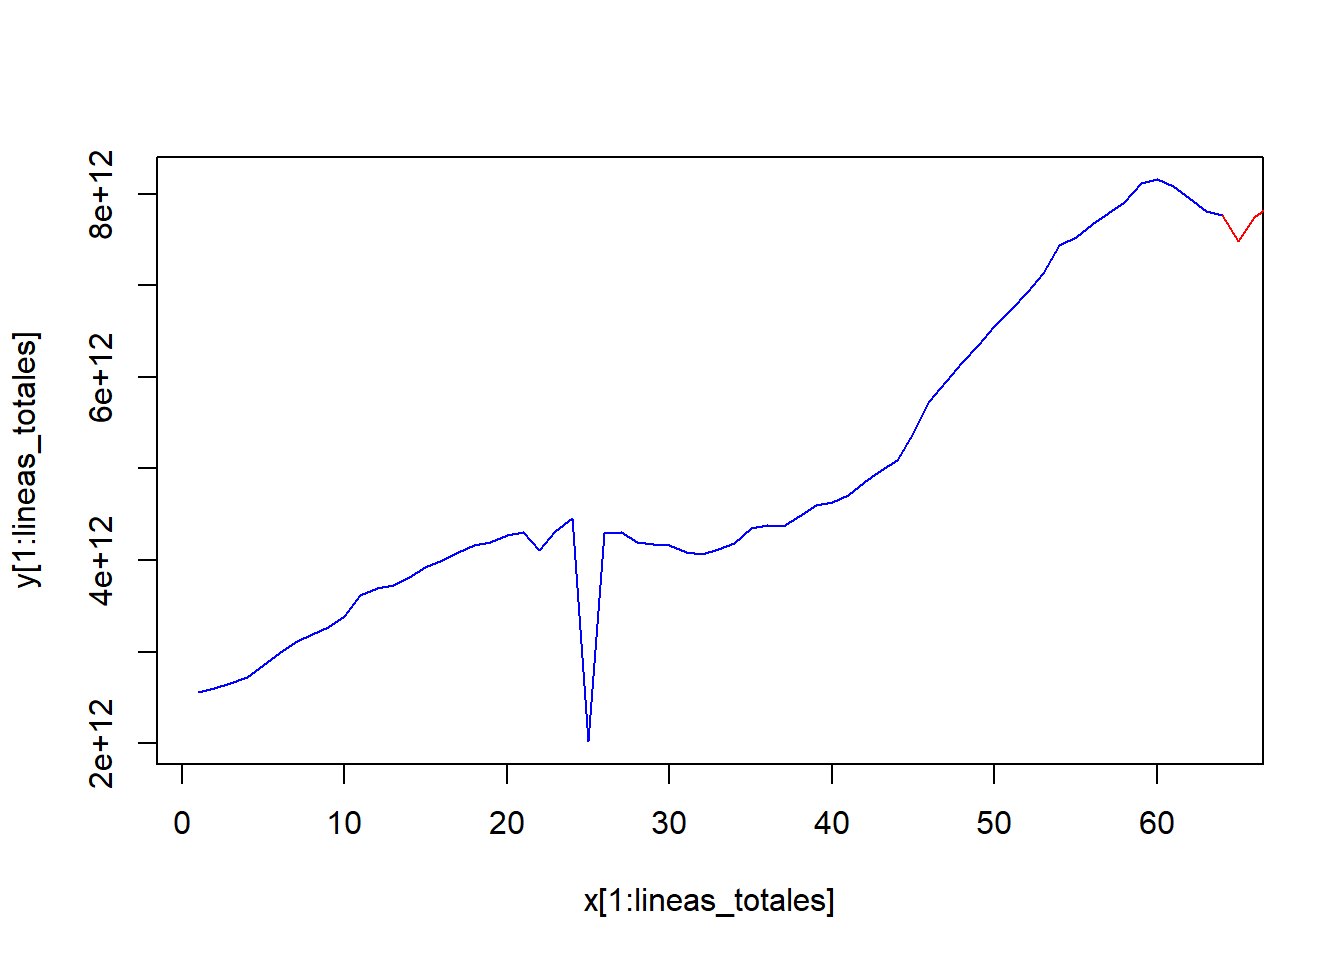
\includegraphics{bookdown-demo_files/figure-latex/unnamed-chunk-52-1.pdf}

\hypertarget{jordan}{%
\section{Jordan}\label{jordan}}

\begin{Shaded}
\begin{Highlighting}[]
\NormalTok{fit}\OtherTok{\textless{}{-}}\FunctionTok{jordan}\NormalTok{(inputs[t\_train],}
\NormalTok{    outputs[t\_train],}
    \AttributeTok{size=}\DecValTok{6}\NormalTok{,}
    \AttributeTok{learnFuncParams=}\FunctionTok{c}\NormalTok{(}\FloatTok{0.01}\NormalTok{),}
    \AttributeTok{maxit=}\DecValTok{100000}\NormalTok{)}
\end{Highlighting}
\end{Shaded}

Ploteamos el error iterativo de 7 neuronas:

\begin{Shaded}
\begin{Highlighting}[]
\FunctionTok{plotIterativeError}\NormalTok{(fit, }\AttributeTok{main =} \StringTok{"Iterative Error for 7 Neuron"}\NormalTok{)}
\end{Highlighting}
\end{Shaded}

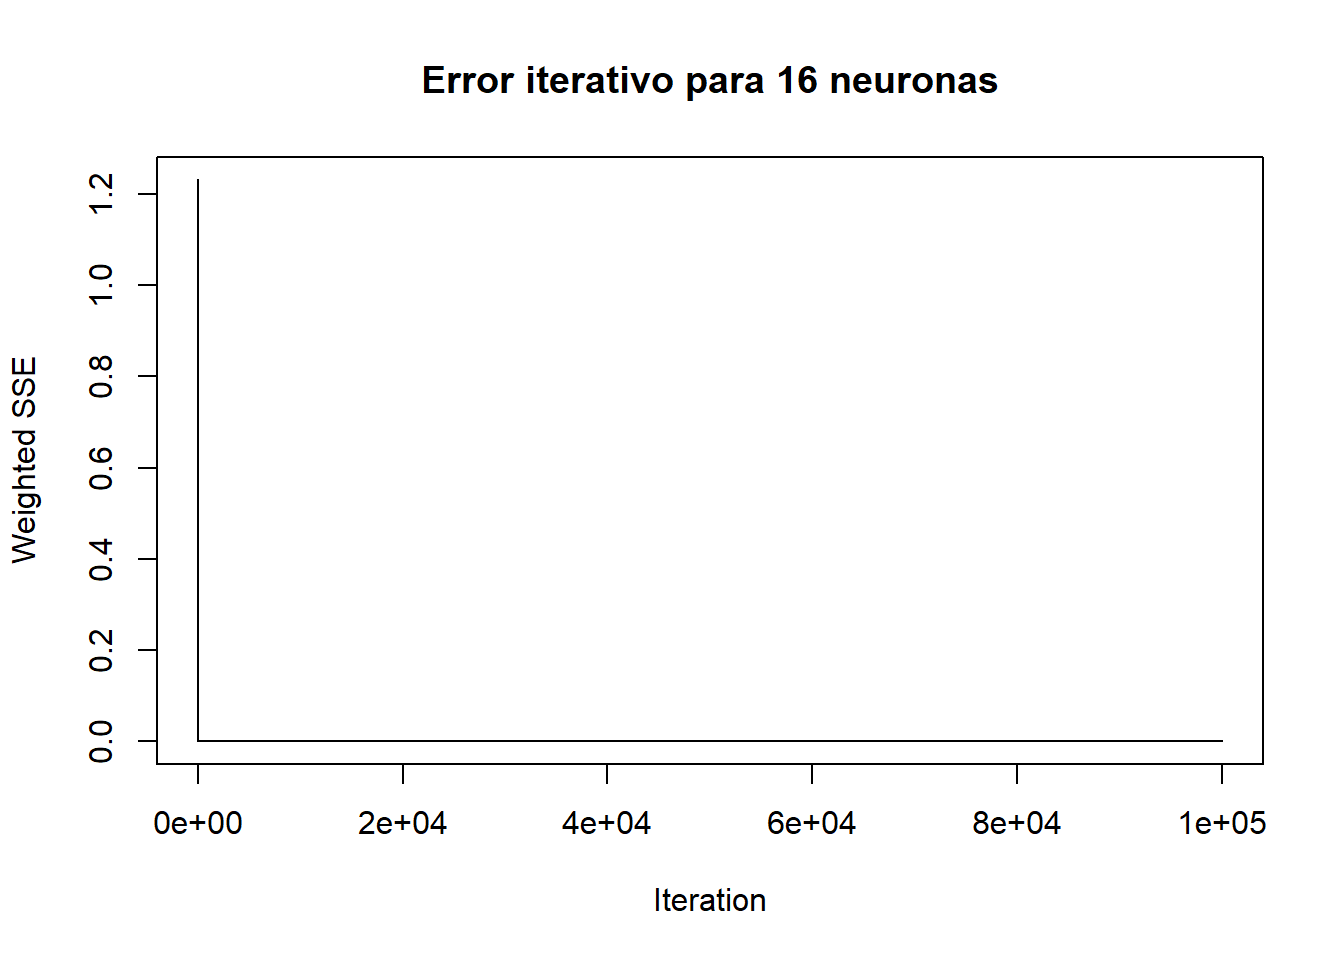
\includegraphics{bookdown-demo_files/figure-latex/unnamed-chunk-54-1.pdf}

Veamos ahora el error

\begin{Shaded}
\begin{Highlighting}[]
\NormalTok{y }\OtherTok{\textless{}{-}} \FunctionTok{as.vector}\NormalTok{(outputs[}\SpecialCharTok{{-}}\NormalTok{t\_test])}
\FunctionTok{plot}\NormalTok{(y,}\AttributeTok{type=}\StringTok{"l"}\NormalTok{)}
\NormalTok{pred }\OtherTok{\textless{}{-}} \FunctionTok{predict}\NormalTok{(fit, inputs[}\SpecialCharTok{{-}}\NormalTok{t\_test])}
\FunctionTok{lines}\NormalTok{(pred,}\AttributeTok{col =} \StringTok{"red"}\NormalTok{)}
\end{Highlighting}
\end{Shaded}

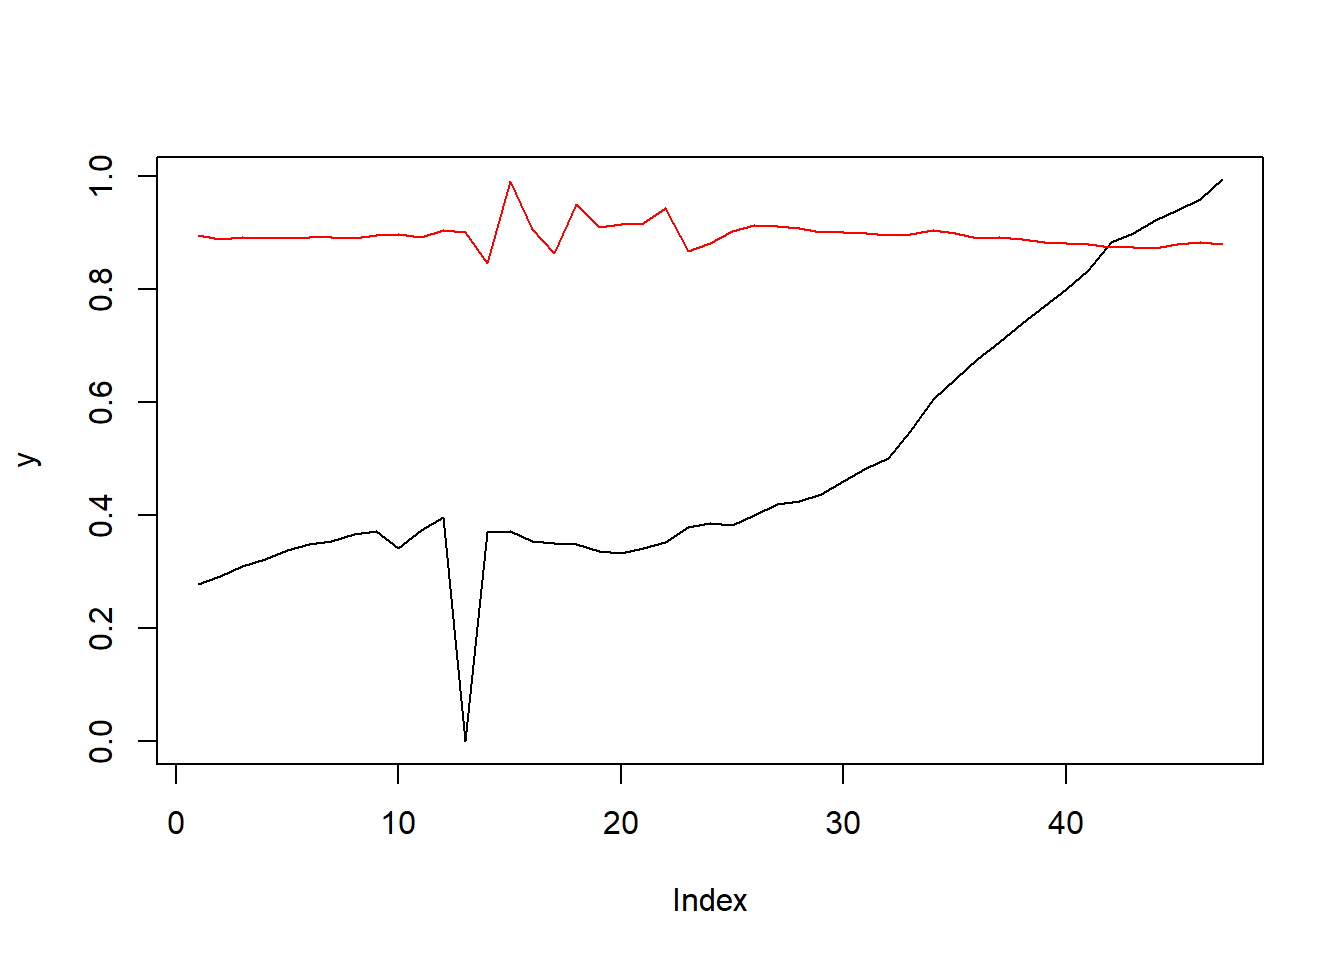
\includegraphics{bookdown-demo_files/figure-latex/unnamed-chunk-55-1.pdf}
Procedemos con la prediccion

\begin{Shaded}
\begin{Highlighting}[]
\NormalTok{predictions }\OtherTok{\textless{}{-}} \FunctionTok{predict}\NormalTok{(fit,inputs[}\SpecialCharTok{{-}}\NormalTok{t\_train])}
\NormalTok{mod\_jordan }\OtherTok{\textless{}{-}}\NormalTok{ predictions}\SpecialCharTok{*}\NormalTok{(}\FunctionTok{max}\NormalTok{(Z)}\SpecialCharTok{{-}}\FunctionTok{min}\NormalTok{(Z))}\SpecialCharTok{+}\FunctionTok{min}\NormalTok{(Z)}
\NormalTok{mod\_jordan}
\end{Highlighting}
\end{Shaded}

\begin{verbatim}
##                  [,1]
## Jan 2019 7.496510e+12
## Feb 2019 7.466085e+12
## Mar 2019 7.485655e+12
## Apr 2019 7.484994e+12
## May 2019 7.482381e+12
## Jun 2019 7.492138e+12
## Jul 2019 7.487598e+12
## Aug 2019 7.476202e+12
## Sep 2019 7.511885e+12
## Oct 2019 7.521976e+12
## Nov 2019 7.491398e+12
## Dec 2019 7.565753e+12
## Jan 2020 7.545399e+12
## Feb 2020 7.212222e+12
## Mar 2020 8.100570e+12
## Apr 2020 7.577544e+12
## May 2020 7.313275e+12
## Jun 2020 7.852690e+12
## Jul 2020 7.598834e+12
## Aug 2020 7.626874e+12
## Sep 2020 7.644746e+12
## Oct 2020 7.805679e+12
## Nov 2020 7.340772e+12
## Dec 2020 7.427901e+12
## Jan 2021 7.561133e+12
## Feb 2021 7.616939e+12
## Mar 2021 7.613438e+12
## Apr 2021 7.586914e+12
## May 2021 7.548052e+12
## Jun 2021 7.545705e+12
## Jul 2021 7.539354e+12
## Aug 2021 7.516734e+12
## Sep 2021 7.527965e+12
## Oct 2021 7.563203e+12
## Nov 2021 7.529698e+12
## Dec 2021 7.477176e+12
## Jan 2022 7.490395e+12
## Feb 2022 7.473057e+12
## Mar 2022 7.439036e+12
## Apr 2022 7.421486e+12
## May 2022 7.410294e+12
## Jun 2022 7.385566e+12
## Jul 2022 7.381260e+12
## Aug 2022 7.371684e+12
## Sep 2022 7.414113e+12
## Oct 2022 7.432210e+12
## Nov 2022 7.416511e+12
## Jan 2023 7.429574e+12
## Feb 2023 7.427371e+12
## Mar 2023 7.454445e+12
## Apr 2023 7.493430e+12
\end{verbatim}

Ahora veamoslo en la grafica

\begin{Shaded}
\begin{Highlighting}[]
\NormalTok{x }\OtherTok{\textless{}{-}} \DecValTok{1}\SpecialCharTok{:}\NormalTok{(lineas\_totales}\SpecialCharTok{+}\FunctionTok{length}\NormalTok{(mod\_jordan))}
\NormalTok{y }\OtherTok{\textless{}{-}} \FunctionTok{c}\NormalTok{(}\FunctionTok{as.vector}\NormalTok{(Z),mod\_jordan)}
\FunctionTok{plot}\NormalTok{(x[}\DecValTok{1}\SpecialCharTok{:}\NormalTok{lineas\_totales], y[}\DecValTok{1}\SpecialCharTok{:}\NormalTok{lineas\_totales],}\AttributeTok{col =} \StringTok{"blue"}\NormalTok{, }\AttributeTok{type=}\StringTok{"l"}\NormalTok{)}
\FunctionTok{lines}\NormalTok{( x[(lineas\_totales)}\SpecialCharTok{:}\FunctionTok{length}\NormalTok{(x)], y[(lineas\_totales)}\SpecialCharTok{:}\FunctionTok{length}\NormalTok{(x)], }\AttributeTok{col=}\StringTok{"red"}\NormalTok{)}
\end{Highlighting}
\end{Shaded}

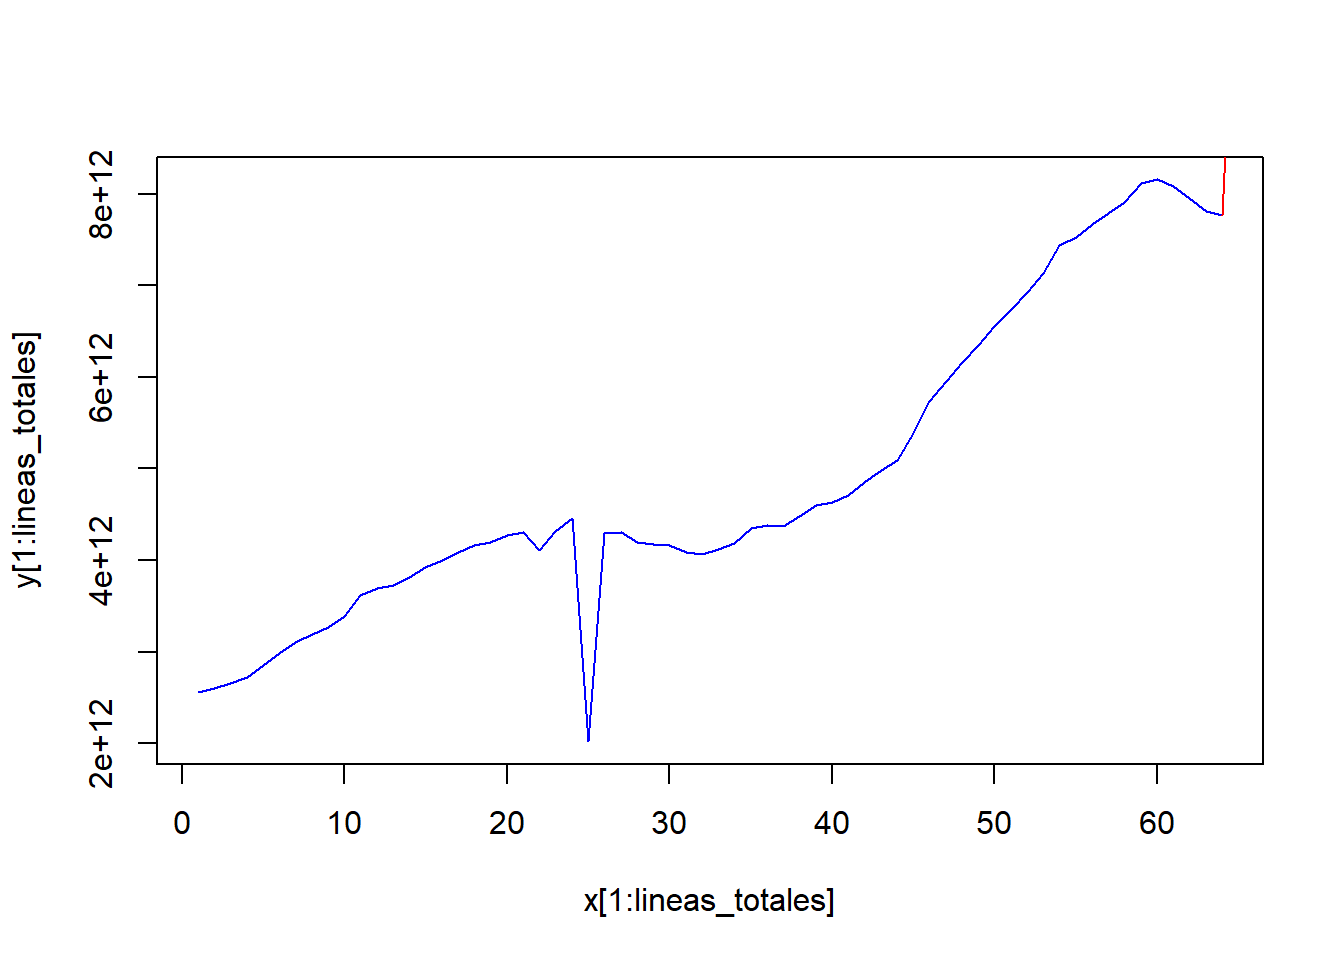
\includegraphics{bookdown-demo_files/figure-latex/unnamed-chunk-57-1.pdf}

  \bibliography{book.bib,packages.bib}

\end{document}
